% 西安科技大学应用统计硕士学位论文
% 版式自旧稿 thesis_main.tex(ctexbook、A4、学校页边距)改造:去掉彩色链接与灰色页眉,
% 标题用黑体而非加粗,字体沿用新稿的回退写法(缺 Times New Roman / SimSun 时回退到
% Liberation Serif 与 Noto Serif CJK SC)。章节正文在 chapters/,sections 为指向它的链接。
\documentclass[fontset=none,zihao=-4,a4paper,twoside,openany]{ctexbook}
\usepackage{iftex}
% 罗马数字Ⅰ/Ⅱ(U+2160 段)Liberation Serif 没有字形,归入 CJK 字符类交给中文字体。
\xeCJKDeclareCharClass{CJK}{"2160 -> "216F}
\ifXeTeX\else
  \PackageError{thesis-template}{XeLaTeX is required}{Run xelatex.}
\fi
\usepackage{fontspec}
\IfFontExistsTF{Times New Roman}{
  \setmainfont{Times New Roman}
}{
  \setmainfont{Liberation Serif}
}
\IfFontExistsTF{SimSun}{
  \setCJKmainfont{SimSun}
}{
  \IfFontExistsTF{Songti SC}{
    \setCJKmainfont{Songti SC}
  }{
    \IfFontExistsTF{STSong}{
      \setCJKmainfont{STSong}
    }{
      \setCJKmainfont{Noto Serif CJK SC}
    }
  }
}
\IfFontExistsTF{SimHei}{
  \setCJKsansfont{SimHei}
  \newCJKfontfamily\heiti{SimHei}
}{
  \IfFontExistsTF{Heiti SC}{
    \setCJKsansfont{Heiti SC}
    \newCJKfontfamily\heiti{Heiti SC}
  }{
    \setCJKsansfont{Noto Sans CJK SC}
    \newCJKfontfamily\heiti{Noto Sans CJK SC}
  }
}
\usepackage{graphicx}
\usepackage{amsmath,amsthm}
\usepackage{unicode-math}
\setmathfont{Latin Modern Math}
% 估计量的帽子用 pict2e 画成矢量折线,与新稿一致。
\usepackage{pict2e}
\newcommand{\hatmark}{{\setlength{\unitlength}{0.1em}\linethickness{0.045em}%
  \begin{picture}(5,1.7)\polyline(0.2,0)(2.5,1.5)(4.8,0)\end{picture}}}
\AtBeginDocument{%
  \renewcommand{\widehat}[1]{\overset{\hatmark}{#1}}%
  \renewcommand{\hat}[1]{\overset{\hatmark}{#1}}}
% 学校页边距:上 3.0、下 2.5、内 3.0、外 2.5 厘米
\usepackage[a4paper,top=3.0cm,bottom=2.5cm,inner=3.0cm,outer=2.5cm,
  headheight=15pt,headsep=18pt,footskip=22pt]{geometry}
\usepackage[numbers,sort&compress]{natbib}
\usepackage{booktabs}
\usepackage{tabularx}
\usepackage{multirow}
\usepackage{microtype}
\usepackage{xcolor}
\usepackage{enumitem}
\usepackage{array}
\usepackage{xurl}
\usepackage[hidelinks,unicode=true,bookmarksnumbered=true]{hyperref}
\urlstyle{same}
\usepackage{caption}
\usepackage{subcaption}
\usepackage{placeins}
\captionsetup{
  font=small,
  labelfont=normalfont,
  textfont=normalfont,
  labelsep=space,
  justification=justified,
  singlelinecheck=true,
  skip=6pt
}
\setlength{\textfloatsep}{12pt plus 2pt minus 2pt}
\setlength{\floatsep}{10pt plus 2pt minus 2pt}
\setlength{\intextsep}{10pt plus 2pt minus 2pt}
\setcounter{topnumber}{5}
\setcounter{bottomnumber}{3}
\setcounter{totalnumber}{8}
\renewcommand{\topfraction}{0.90}
\renewcommand{\bottomfraction}{0.80}
\renewcommand{\textfraction}{0.07}
\renewcommand{\floatpagefraction}{0.70}
\setlist{nosep,leftmargin=2em}
\linespread{1.3}

% 章节标题:黑体,不加粗
\ctexset{
  chapter = {
    format = \centering\heiti\zihao{3},
    name = {第,章},
    number = \chinese{chapter},
    aftername = \quad,
    beforeskip = 12pt,
    afterskip = 24pt
  },
  section = {
    format = \heiti\zihao{4},
    beforeskip = 16pt plus 2pt minus 2pt,
    afterskip = 10pt plus 2pt minus 2pt
  },
  subsection = {
    format = \heiti\zihao{-4},
    beforeskip = 12pt plus 2pt minus 2pt,
    afterskip = 8pt plus 2pt minus 2pt
  },
  subsubsection = {
    format = \heiti\zihao{-4},
    beforeskip = 8pt plus 2pt minus 2pt,
    afterskip = 6pt plus 2pt minus 2pt
  },
  bibname = {参考文献},
  contentsname = {目\quad 录},
  listfigurename = {插图清单},
  listtablename = {表格清单},
  appendixname = {附录}
}

% 页眉:学位论文格式要求双面页眉,偶数页为论文类别,奇数页为当前章标题,黑色。
% qa-allow-chinese-running-header: 西安科技大学学位论文格式要求奇偶页页眉
\usepackage{fancyhdr}
\fancypagestyle{thesis}{%
  \fancyhf{}%
  \fancyhead[CE]{\small 西安科技大学硕士学位论文}%
  \fancyhead[CO]{\small \leftmark}%
  \fancyfoot[C]{\small\thepage}%
  \renewcommand{\headrulewidth}{0.5pt}%
  \renewcommand{\footrulewidth}{0pt}}
\fancypagestyle{plain}{%
  \fancyhf{}%
  \fancyhead[CE]{\small 西安科技大学硕士学位论文}%
  \fancyhead[CO]{\small \leftmark}%
  \fancyfoot[C]{\small\thepage}%
  \renewcommand{\headrulewidth}{0.5pt}%
  \renewcommand{\footrulewidth}{0pt}}
\renewcommand{\chaptermark}[1]{\markboth{\ifnum\value{chapter}>0 \CTEXthechapter\quad\fi #1}{}}
\renewcommand{\sectionmark}[1]{}

% 定理类环境:按章编号,标题黑体
\newtheoremstyle{zhplain}{0.6em}{0.6em}{\normalfont}{}{\heiti}{}{0.8em}{}
\theoremstyle{zhplain}
\newtheorem{proposition}{命题}[chapter]
\newtheorem{corollary}{推论}[chapter]
\newtheorem{lemma}{引理}[chapter]
\newtheorem{definition}{定义}[chapter]
\newtheorem{remark}{注}[chapter]
\renewcommand{\proofname}{证明}
\makeatletter
\renewenvironment{proof}[1][\proofname]{\par\pushQED{\qed}\normalfont
  \topsep6\p@\@plus6\p@\relax\trivlist
  \item[\hskip\labelsep\heiti #1\@addpunct{：}]\ignorespaces}{\popQED\endtrivlist\@endpefalse}
\makeatother
\numberwithin{equation}{chapter}
\renewcommand{\theequation}{\thechapter.\arabic{equation}}
\renewcommand{\thefigure}{\thechapter-\arabic{figure}}
\renewcommand{\thetable}{\thechapter-\arabic{table}}

\newcommand{\Rbar}{\overline{R}}
\newcommand{\mx}{m_{\times}}
\newcommand{\NB}{\operatorname{NB}}
\newcommand{\Var}{\operatorname{Var}}
\newcommand{\E}{\operatorname{E}}
\newcommand{\RelMSE}{\operatorname{RelMSE}}
\newcommand{\Cov}{\operatorname{Cov}}
\newcommand{\CV}{\operatorname{CV}}
\newcommand{\Bin}{\operatorname{Bin}}

% 盲审开关:送盲审时改为 \blindtrue,封面姓名、学号与导师即隐去。
\newif\ifblind
\blindfalse

\title{疫情监测中的病例规模收益边界：估计目标、环境随机性与外部验证}
\newcommand{\entitle}{Returns to Case-Count Scale in Epidemic Surveillance: Estimation Targets, Environmental Stochasticity and External Validation}
\date{}

% 封面由 \maketitle 生成
\makeatletter
\renewcommand{\maketitle}{%
  \begin{titlepage}
    \thispagestyle{empty}
    {\small
    \begin{tabular}{@{}ll@{}}
      学校代码：& 10704 \\
      学\qquad 号：& \ifblind ＿＿＿＿＿＿ \else 24201221020\fi \\
      分\ 类\ 号：& ＿＿＿＿＿＿ \\
      密\qquad 级：& 公开 \\
    \end{tabular}\par}
    \vspace*{2.2cm}
    \begin{center}
      {\heiti\zihao{1} 硕士学位论文\par}
      \vspace{0.6cm}
      {\zihao{4} 专业学位\par}
      \vspace{2.0cm}
      {\heiti\zihao{2} 疫情监测中的病例规模收益边界：\par}
      \vspace{0.3cm}
      {\heiti\zihao{3} 估计目标、环境随机性与外部验证\par}
      \vspace{0.8cm}
      {\zihao{4}\begin{minipage}{0.86\textwidth}\centering\entitle\end{minipage}\par}
      \vspace{2.4cm}
      {\zihao{-3}
      \renewcommand{\arraystretch}{1.5}
      \begin{tabular}{@{}r@{\quad}l@{}}
        作者姓名：& \ifblind （盲审隐去）\else 王驰\fi \\
        专业学位类别：& 应用统计硕士 \\
        研究方向：& 传染病监测数据的统计建模 \\
        校内导师：& \ifblind （盲审隐去）\else 张仲华\fi \\
        培养单位：& 西安科技大学 \\
      \end{tabular}\par}
      \vfill
      {\zihao{-3} 二〇二六年十月\par}
    \end{center}
  \end{titlepage}}
\makeatother

\begin{document}
\frontmatter
\pagestyle{empty}
\maketitle\normalfont\mdseries

\chapter*{学位论文原创性声明和知识产权声明}
本人郑重声明：本论文是在导师指导下独立完成的研究工作。除文中已经注明引用的内容外，本论文不包含他人已经发表或撰写的研究成果。论文相关数据、代码和推导均按文中所述来源与方法处理。

本人同意学校按照有关规定保存、使用和汇编本论文，并同意在规定范围内提供检索和阅览服务。涉及保密内容的，按学校相关规定执行。

\vspace{2cm}
\begin{tabular}{@{}ll@{}}作者签名：\rule[-2pt]{3cm}{0.4pt} & 日期：\rule[-2pt]{3cm}{0.4pt}\end{tabular}

\cleardoublepage
\pagestyle{thesis}
\pagenumbering{Roman}
\chapter*{摘要}
\addcontentsline{toc}{chapter}{摘要}

疫情监测通常默认报告病例越多，对传播水平的估计越准确。本文研究这一判断在什么条件下成立，以及规模收益的边界在哪里。

本文在负二项传播与二项报告的单代模型下区分两个估计目标。若目标是当期再生数，估计量 $C_t/(\rho n)$ 是极大似然估计，在任意有限规模下达到 Cram\'er--Rao 下界，并且是一致最小方差无偏估计，误差随规模趋于零。若目标是跨期平均再生数，估计量的方差分解为环境项 $v_R$ 与规模项 $A/m$ 之和，扩大规模只能消除后者，环境方差构成规模无法突破的底板。规模项等于环境项时的预计报告规模 $\mx=A/v_R$ 称为交叉点，它把环境底板折算成病例数。按文献中的住院监测情景参数，交叉点为每期 21.3--49.2 例报告。由方差结构可以得到三类设计结论。总报告量固定时期数越多越好，环境的正自相关会使常用的有效期数近似高估环境项。存在每期固定成本时，最优单期规模是交叉点与成本比乘积的平方根。判断当期增长时，基于负二项分布的精确检验可以控制水平，稳定检出 15\% 的增长约需示例交叉点十倍的规模。更新过程仿真表明，单代公式在时间序列中只能作为参照曲线。

实证部分使用美国 51 个辖区截至 2026 年 9 月的州级流感住院周报，以更新分母下的周增长比构造单步预测损失。流行初期，相对均方误差随实际规模下降并趋于常数。仿射拟合的截距为 0.0991，斜率为 2.243，1,500 次按州聚类重抽的斜率全部为正，经验交叉点为 22.6 例/周。拟合系数都是情景隐含值的三倍以上，只能检验误差形状，不能作为结构参数的估计。分母中的二项报告噪声按滞后权重平方和抬高斜率而不改变截距，可解释斜率水平的一半左右，本文给出这一抬高的一阶推导并用模拟核对。达峰期以初期基准预测时，88.9\% 的损失来自基准偏移；自愿填报期周增长比的标准差扩张 192\%，稳健离散度基本不变。工具变量、事前基准、时变基准以及 FluSight 集成预测和欧洲 COVID-19 两组外部数据下，规模项都为正，经验交叉点在 10.6--124.7 之间变化，只宜作量级参考。全国汇总序列的损失约为州级截距的三分之一，说明空间汇总能降低环境底板。

研究表明，监测设计应先明确估计目标：预警类问题需要尽可能大的规模，趋势类问题在规模达到交叉点量级后，应把资源转向增加观测期数、汇总辖区和更新基准模型。

\vspace{1em}
\noindent\heiti 关键词：\normalfont 病例规模；再生数；估计目标；环境随机性；交叉点；流感住院监测

\chapter*{Abstract}
\addcontentsline{toc}{chapter}{Abstract}

Epidemic surveillance often assumes that more reported cases always yield more precise estimates of transmission. This thesis asks when that assumption holds and where the returns to case-count scale end.

Under a single-generation model with negative-binomial offspring and binomial reporting, two estimation targets are distinguished. For the current reproduction number, the estimator $C_t/(\rho n)$ is the maximum-likelihood estimator, attains the Cram\'er--Rao bound at every finite scale, and is the uniformly minimum-variance unbiased estimator, so its error vanishes as scale grows. For the average reproduction number across periods, the variance splits into an environmental term $v_R$ and a scale term $A/m$; scale removes only the latter, and environmental variance sets a floor. The crossover scale $\mx=A/v_R$, at which the two terms are equal, expresses this floor as a case count; under literature-based scenarios for hospital surveillance it lies between 21.3 and 49.2 reported cases per period. The variance structure yields three design results. With a fixed total, more periods are better, and positive autocorrelation makes the usual effective-sample-size approximation overstate the environmental term. With a fixed cost per period, the optimal per-period scale is the square root of the crossover scale times the cost ratio. An exact negative-binomial test controls size when detecting growth, although detecting a 15\% increase reliably needs about ten times the crossover scale of the worked example. Renewal-process simulations show that the single-generation formula serves only as a reference curve in time series.

The empirical analysis uses weekly state-level influenza hospitalization reports from 51 United States jurisdictions through September 2026 and builds one-step forecast losses from weekly growth ratios with a renewal denominator. In the early epidemic phase the relative mean squared error falls with realized scale and levels off. The affine fit has intercept 0.0991 and slope 2.243, all 1,500 state-cluster bootstrap slopes are positive, and the empirical crossover is 22.6 cases per week. Both coefficients exceed the scenario values by a factor of more than three, so the fit tests the shape of the error curve rather than structural parameters. Binomial reporting noise in the denominator raises the slope in proportion to the sum of squared lag weights while leaving the intercept unchanged, accounting for about half of the slope; a first-order derivation is given and checked by simulation. Near the peak, 88.9\% of the loss under the early-phase baseline comes from baseline shift, and during voluntary reporting the standard deviation of growth ratios expands by 192\% while robust dispersion stays nearly constant. The scale term remains positive under instrumental variables, ex-ante and time-varying baselines, the FluSight ensemble and European COVID-19 data, whereas the empirical crossover ranges from 10.6 to 124.7 and should be read only as an order of magnitude. The loss of the national aggregate is about one third of the state-level intercept, indicating that spatial pooling lowers the environmental floor.

Surveillance design should therefore begin with the estimation target. Early warning benefits from as much scale as possible; once trend estimation reaches the crossover scale, resources are better spent on more periods, pooling across jurisdictions and updating baseline models.

\vspace{1em}
\noindent\textbf{Keywords:}\ \sloppy case-count scale; reproduction number; estimation target; environmental stochasticity; crossover scale; influenza hospitalization surveillance


\tableofcontents
\listoffigures
\listoftables

\mainmatter
\pagestyle{thesis}
\chapter{绪\quad 论}\label{ch:introduction}

\section{研究背景与问题提出}\label{sec:background}

\subsection{传染病监测的世纪演进：从宏观仓室到微观统计推断}
自二十世纪初近代数理流行病学创立以来，定量刻画传染病传播动态、评估防控干预成效一直是应用数学、统计学与公共卫生交叉领域的核心前沿。1927 年，Kermack 与 McKendrick 提出了划时代的确定性仓室易感--感染--移出（SIR）常微分方程模型 \citep{kermack1927contribution}，首次奠定了通过微分方程动力系统定性理论研究传染病临界暴发阈值的理论根基。在过去的近一个世纪中，以 Anderson 与 May \citep{anderson1991infectious}、Hethcote \citep{hethcote2000mathematics} 以及马知恩先生学派 \citep{ma2001stability,ma2004epidemic} 为代表的学者们，将常微分方程稳定性理论、下一代矩阵法 \citep{diekmann1990definition,diekmann2000mathematical} 与分岔分析深入引入传染病动力学，确立了基本再生数 $\mathcal{R}_0$ 作为无病平衡点局部与全局渐近稳定性的核心判据。

然而，经典确定性微分方程仓室模型本质上依赖于“大数定律完全成立”的流体极限假定（Fluid Limit Theorem）\citep{kurtz1970solutions,kurtz1971limit}，即假设易感人群与感染人群规模无限大、个体接触完全均匀混合、系统演化完全遵循确定性均值轨道。进入二十一世纪，随着全球化人口流动加剧、新型呼吸道病原体（如 SARS、高致病性禽流感、H1N1 新型流感及 COVID-19）频繁爆发，真实疫情传播展现出高度复杂的随机性特征。一方面，真实世界中的传染病暴发始于少数感染个体的微观随机链式反应，必须借助随机生灭过程与 Galton--Watson 分支过程进行建模 \citep{harris1963theory,jagers1975branching,britton2010stochastic}；另一方面，流行病学决策者往往无法直接观测到全社会底层的全部感染状态，只能通过哨点医院网络记录到带有严重滞后与漏报的病例计数时序序列。

在此背景下，传染病监测的推断范式经历了从“基于大样本长时程拟合静态参数”向“基于实时观测病例流估计时变瞬时再生数 $R_t$”的深刻转变。时变再生数 $R_t$ 定义为在 $t$ 时刻特定的防控干预、气象环境与人群行为条件下，平均一个感染者引发的二次感染人数。由于 $R_t = 1$ 精确对应了动力系统在相空间中的稳定临界分界线，实时监测 $R_t$ 是否越过 1 成为指导学校停课、医疗资源调度与口罩令实施的关键决策指针。

\subsection{公共卫生应急决策中的“规模崇拜”困境与现实悖论}
伴随现代生物检测技术通量的激增与数字化疫情直报网络的普及，公共卫生监测实践中普遍滋生了一种强烈的经验预设，即所谓的**“监测规模崇拜”**（Surveillance Scale Worship）。这一直觉认为：
\begin{quote}
\textit{“捕获的数据越多越好，样本量越大推断越准。只要疾控机构不断增加检测哨点、扩大医院上报覆盖面、增加报告确诊人数（即增大病例样本规模 $m$），统计推断与前瞻预测的不确定性就能被无界压缩。”}
\end{quote}
这一直觉在纯粹的数理统计抽样理论中似乎不言自明——大数定律与中心极限定理指出，独立同分布样本均值的估计方差随样本量按 $O(1/m)$ 速率严格递减，因此投入更多资源捕获更多病例，理应获得更高的预测精度。

然而，在多次全球性重大传染病暴发的应对实务中，世界卫生组织（WHO）及各国疾控中心频繁陷入极其尴尬的现实困境：
\begin{enumerate}[label=(\arabic*)]
    \item **高峰期预测精度平台瓶颈**：在疫情高发暴发期，医疗监测系统每周能捕获成千上万例确诊住院病例，但前瞻预测模型的相对误差往往依然居高不下；
    \item **边际扩网收益锐减**：卫生部门投入巨额财政资金成倍扩建检测网络后，对未来趋势判断的改善却极其微弱，迅速陷入明显的平台钝化期；
    \item **资源错配困境**：在疫情低发期或早期，由于病例稀疏，系统饱受抽样噪声干扰而频繁产生虚警或漏报；而在高发期，巨额采样资源堆积在已被证实处于饱和状态的大型医院，造成基层流调资源的严重浪费。
\end{enumerate}

面对这一现实矛盾，流行病学界以往多笼统地归咎于“医院瞒报漏报”、“公众就医行为改变”或“具体预测模型结构设定不当”。但这些定性解释始终未能回答一个根本性的数学与统计学科学设问：
\begin{center}
\textbf{在资源受限情境下，无限扩大病例报告规模的边际方差收益何时递减？\\微观抽样误差与宏观环境噪声究竟如何抗衡？\\是否存在一个内生决定且可严格解析计算的特征规模临界平衡点？}
\end{center}

\section{国内外研究现状与文献综述}\label{sec:literature}

为了系统厘清上述科学设问的学术渊源，本节系统梳理时变再生数估计、超传播离散建模、信息论极限及运筹抽样设计的既有研究脉络，并剖析既有理论的关键缺口。

\subsection{时变再生数估计方法的演进历程}
在实时再生数估计领域，早期的经典方法依赖于回顾性代际追踪。Wallinga 与 Teunis \citep{wallinga2004different} 提出了基于病例对（Pairwise）相对发病时间间隔概率的拟似然估计法（WT 方法）。然而，WT 方法本质上估计的是“病例队列再生数”（Case Reproduction Number），即一个特定发病日期的感染者在其整个病程中引发的总后续感染数，这导致其在疫情当周无法实时结算，必须等待一个完整潜伏传播周期后才能完成回顾性后验修正，存在长达数周的结构性时滞 \citep{cauchemez2006real,fraser2007estimating}。

为了消除这一回顾性时滞，Fraser \citep{fraser2007estimating} 提出了基于更新方程（Renewal Equation）的瞬时再生数理论框架。在假定感染代际时间（Generation Time）分布已知的前提下，当期新发感染数可表示为历史感染压力的加权卷积：
\begin{equation}
I_t = R_t \sum_{s=1}^t I_{t-s} w_s,
\end{equation}
其中 $w_s$ 为代际间隔概率密度。随后，Cori 等人 \citep{cori2013new} 在《American Journal of Epidemiology》上发表了标志性的 EpiEstim 框架。EpiEstim 假设在滑动的局部时间窗口 $\tau$ 内传播强度恒定，假定观测病例在给定历史卷积压力下服从泊松分布，并利用共轭 Gamma 先验导出了后验分布的解析闭式解。Thompson 等人 \citep{thompson2019improved} 进一步将该框架推广至考虑输入病例与本土病例分化的场景；Gostic 等人 \citep{gostic2020practical} 则系统评估了就医填报时滞反卷积平滑对 EpiEstim 稳定性的影响。

然而，EpiEstim 及其衍生方法的核心假设均建立在**“条件独立泊松分布”**之上。在数理统计上，泊松分布强制方差等于均值，这一假定严重忽略了真实人类传染病中普遍存在的微观超传播特征。

\subsection{微观生物学超传播与过度离散建模}
真实传染病的传播过程绝非均匀微观相遇。2005 年，Lloyd-Smith 等人 \citep{lloydsmith2005superspreading} 在《Nature》上发表了奠基性论文，通过对全球 8 种传染病的历史个体接触追踪数据进行元分析，证实人类传染病普遍遵循“20/80 法则”——即大约 20\% 的高感染力个体引发了全社会 80\% 的二次感染事件（所谓的“超级传播事件”，Superspreading Events, SSEs）。

Lloyd-Smith 等人提出用 **负二项分支过程（Negative Binomial Branching Process）** 替代经典泊松分支过程，其微观机制是个体感染力服从 Gamma 混合泊松分布：
\begin{equation}
Y_{t,j} \mid \nu_{t,j} \sim \Poisson(\nu_{t,j}), \quad \nu_{t,j} \sim \GammaDist\left(k, \frac{R_t}{k}\right),
\end{equation}
从而积分边缘化导出个体子代二元分布 $Y_{t,j} \sim \NB(k, \frac{k}{k+R_t})$，其方差结构为：
\begin{equation}
\Var(Y_{t,j}) = R_t + \frac{R_t^2}{k}.
\end{equation}
在此模型中，$k$ 被定义为**生物学生殖数过度离散参数**（Dispersion Parameter）。当 $k \to \infty$ 时，模型退化为经典泊松分布；当 $k \to 0$ 时，模型表现出极端的重尾特征。随后的 COVID-19 大流行研究中，Endo 等 \citep{endo2020estimating}、Althouse 等 \citep{althouse2020superspreading} 及 Sneppen 与 Simonsen \citep{sneppen2021overdispersion} 广泛证实新型冠状病毒的离散参数极低（$k \approx 0.1 \sim 0.3$），表现出极强的超传播倾向。

过度离散特性的引入，意味着微观传染具有极高的重尾随机涨落。如果疾控系统收集到的样本量有限，少量超级传播者的出现或缺席将引发剧烈的抽样方差，常规渐近正态近似将在小计数区间彻底失真。

\subsection{信息论极限与既有文献的关键缺口}
近年来，物理学家与应用数学家开始尝试利用信息论工具探究带噪疫情曲线的推断极限。2022 年，牛津大学的 Parag 等人 \citep{parag2022fundamental} 在《Nature Physics》上发表封面论文《Fundamental limits on inferring epidemic dynamics from noisy case count data》，利用 Fisher 信息矩阵（Fisher Information Matrix）与 Cramér--Rao 下界，系统推导了在不完全报告与观测噪声下估计再生数的信息量上限。

Parag 等人的核心结论表明：观测曲线所包含的 Fisher 信息量 $\mathcal{I}(R_t)$ 随观测病例数近似呈线性增长。这一结论在物理学界引起了广泛关注，但其推导隐含了一个关键前提——**其推断目标始终锚定在“当期特定微观环境下的瞬态参数 $R_t$”**。

这正是既有文献留下的**最致命的理论断裂与盲区**：
\begin{enumerate}[label=(\alph*)]
    \item **推断目标的严重混淆**：
    实际公共卫生决策者需要的往往不是某一周受微观偶然扰动影响的单期瞬态抖动值 $R_t$，而是能够反映潜在流行趋势、消除单周气象或节假日偶发波动的**跨期平稳传播基准 $\bar{R}$**。既有文献从未区分这两个目标在方差标度律上的本质分化。
    \item **忽视不可约宏观环境噪声**：
    在宏观动力学系统中，除了个体抽样的人口统计随机性（Demographic Stochasticity）外，全社会所有感染者不可避免地共同暴露于宏观气象变迁、社会流动潮汐与政策突变等**不可约环境随机性（Environmental Stochasticity）**之下。当估计跨期基准时，单期样本无论扩大到多大，本质上都只能捕获该宏观环境在该期的一个实现值！
    \item **缺乏运筹维度的经济学对偶**：
    既有流行病学研究多停留在“被动给定样本下评估误差”，鲜有将统计推断方差分解与实际监测网络的运作预算、时间抽样期数与单期规模进行联合运筹优化。
\end{enumerate}

表~\ref{tab:literature_comparison} 系统总结了本文与既有标志性文献在建模维度与推断性质上的本质对比。

\begin{table}[htbp]
\centering
\small
\caption{本文与既有核心文献在模型机制与推断理论维度的系统对比}
\label{tab:literature_comparison}
\begin{tabularx}{\textwidth}{lXXXX}
\toprule
\textbf{比较维度} & \textbf{经典仓室 ODE (Kermack)} & \textbf{EpiEstim 框架 (Cori 2013)} & \textbf{信息论界限 (Parag 2022)} & \textbf{本文理论框架} \\
\midrule
\textbf{微观生成机制} & 宏观确定性连续流体 & 条件独立泊松分布 & 状态空间观测模型 & 负二项超传播分支过程 \\
\textbf{宏观报告环节} & 假定完全无偏报告 & 静态先验平滑假定 & 独立乘性高斯/泊松噪声 & 条件二项报告抽稀保族过程 \\
\textbf{核心推断目标} & 静态渐近参数 $\mathcal{R}_0$ & 局部滑窗时变 $R_t$ & 单期瞬态连续参数 $R_t$ & **区分瞬态 $R_t$ 与跨期基准 $\bar{R}$** \\
\textbf{环境变异考量} & 无（确定性流形） & 无（完全吸收入先验） & 视为普通可加测量噪声 & **显式建模不可约环境方差 $v_R$** \\
\textbf{规模收益结论} & 无样本规模维度 & 样本越大后验方差越小 & 信息量随病例数线性增长 & **存在内生特征平衡点 $m_\times$** \\
\textbf{运筹成本对偶} & 无 & 无 & 无 & **同构于 Cochran 两阶段抽样** \\
\textbf{真实大数据检验} & 历史唯象拟合 & 局部小样本演示 & 数值仿真为主 & **全美 1.6 万记录与外部多病种** \\
\bottomrule
\end{tabularx}
\end{table}

\section{本文研究动机与核心科学贡献}\label{sec:contribution}

\subsection{核心研究动机}
立足于上述理论断裂与现实困境，本文旨在打破“规模越大越好”的传统单一教条，建立一套贯通**“微观超传播分支过程 $\to$ 宏观二项报告抽稀 $\to$ 渐近推断方差分解 $\to$ 运筹抽样设计 $\to$ 真实大数据计量检验”**的完整理论与实证闭环体系，精准回答流行病学监测资源何时应当由“单纯扩充数量”转向“结构性协同提质”。

\subsection{主要学术贡献}
本文的核心学术创新可概括为以下四项支柱性贡献：

\begin{enumerate}[label=\textbf{\arabic*.}]
    \item **理论框架破局：确立“推断目标决定规模收益”的方差标度律分化**\\
    本文从微观概率母函数（PGF）复合律出发，严密证明了负二项分支过程在二项抽样下具有严格的分布族封闭性。在此基石上，本文证明：
    若目标为当期瞬态再生数 $R_t$（目标 A），估计量方差达到 Cramér--Rao 下界并随规模 $m$ 按 $O(1/m)$ 无界衰减；
    若目标为跨期基础传播基准 $\bar{R}$（目标 B），全方差分解严格导出了包含不可约环境方差底板 $v_R$ 的仿射损失结构：
    \begin{equation}
    \Var = v_R + \frac{A}{m},
    \end{equation}
    并内生导出了刻画人口统计随机性向环境随机性跃迁的特征规模平衡点 $m_\times \equiv A/v_R$。
    
    \item **运筹机制创新：证明监测杠杆非对称性与 Cochran 两阶段抽样对偶**\\
    在监测杠杆比较上，本文严格证明了提高报告率 $\rho \to 1$ 无法突破微观泊松与超传播方差下界，而扩大风险基数 $n \to \infty$ 方可使方差收敛至 $v_R$。
    在运筹设计上，本文证明在固定总样本人数预算 $B = T m$ 下微观抽样误差恒为常数 $A/B$；并在显式经费预算约束 $\mathcal{B} = T(c_0 + c_1 m)$ 下证明了目标方差函数的严格凸性，推导出最优单期规模闭式解 $m^* = \sqrt{\frac{c_0}{c_1} m_\times}$，在数学结构上完美同构于经典抽样调查 Cochran 两阶段最优分配模型。
    
    \item **数理与仿真深化：解析离散功效锯齿波与更新过程预测双口径机制**\\
    针对爆发早期假设检验 $H_0: R_t \le 1$，本文证明单调似然比（MLR）一阶对数差分严格为正，利用 Karlin--Rubin 定理构造了 UMP 检验，揭示了离散计数阶梯跳跃引发的功效锯齿波机制，证实检验目标存在天然饱和天花板 $m_{80\%}$。在更新过程时间序列预测中，推导了条件预测方差分解式，阐明了用历史卷积代理真实感染所必然引入的额外非负预测偏差项，彻底澄清了初始参数口径与实际实现规模口径下的参照收敛性。
    
    \item **真实大数据实证：全美六年流感住院实证反转与外部多病种跨场景验证**\\
    基于全美 CDC NHSN 覆盖 50 州及 DC 长达六年的 16,218 条真实住院面板数据（客观筛选 10,303 个活跃周），采用可行广义最小二乘法（FGLS）与 1,500 次聚类 Bootstrap 检验，证实规模反比项高度显著为正（$\hat{b} = 2.2434$，CI $[1.50, 3.02]$），经验平衡点约为 22.6 例/周。
    均值--方差正交分解惊人地揭示，达峰期看似恒定的高误差中 88.9\% 源于基准失配，扣除后规模项依然显著有用，有力推翻了“达峰期样本量失效”的传统误读；
    进一步引入 CDC FluSight 官方集成预测（达峰偏差从 88.9\% 骤降至 15.5\%）与欧洲 11 国 COVID-19 数据，证实了多模型集成对系统漂移的校准价值及仿射规律跨病种的稳健性。
\end{enumerate}

\section{论文结构安排与技术路线}\label{sec:outline}

为系统展现本文的逻辑流向与整体研究脉络，图~\ref{fig:technical_roadmap_ch1} 给出了贯通全书的“多源输入 $\to$ 微观分支机制 $\to$ 渐近推断方差理论 $\to$ 运筹优化设计 $\to$ 真实大数据实证与政策矩阵”的端到端技术路线全景架构。

\begin{figure}[htbp]
\centering
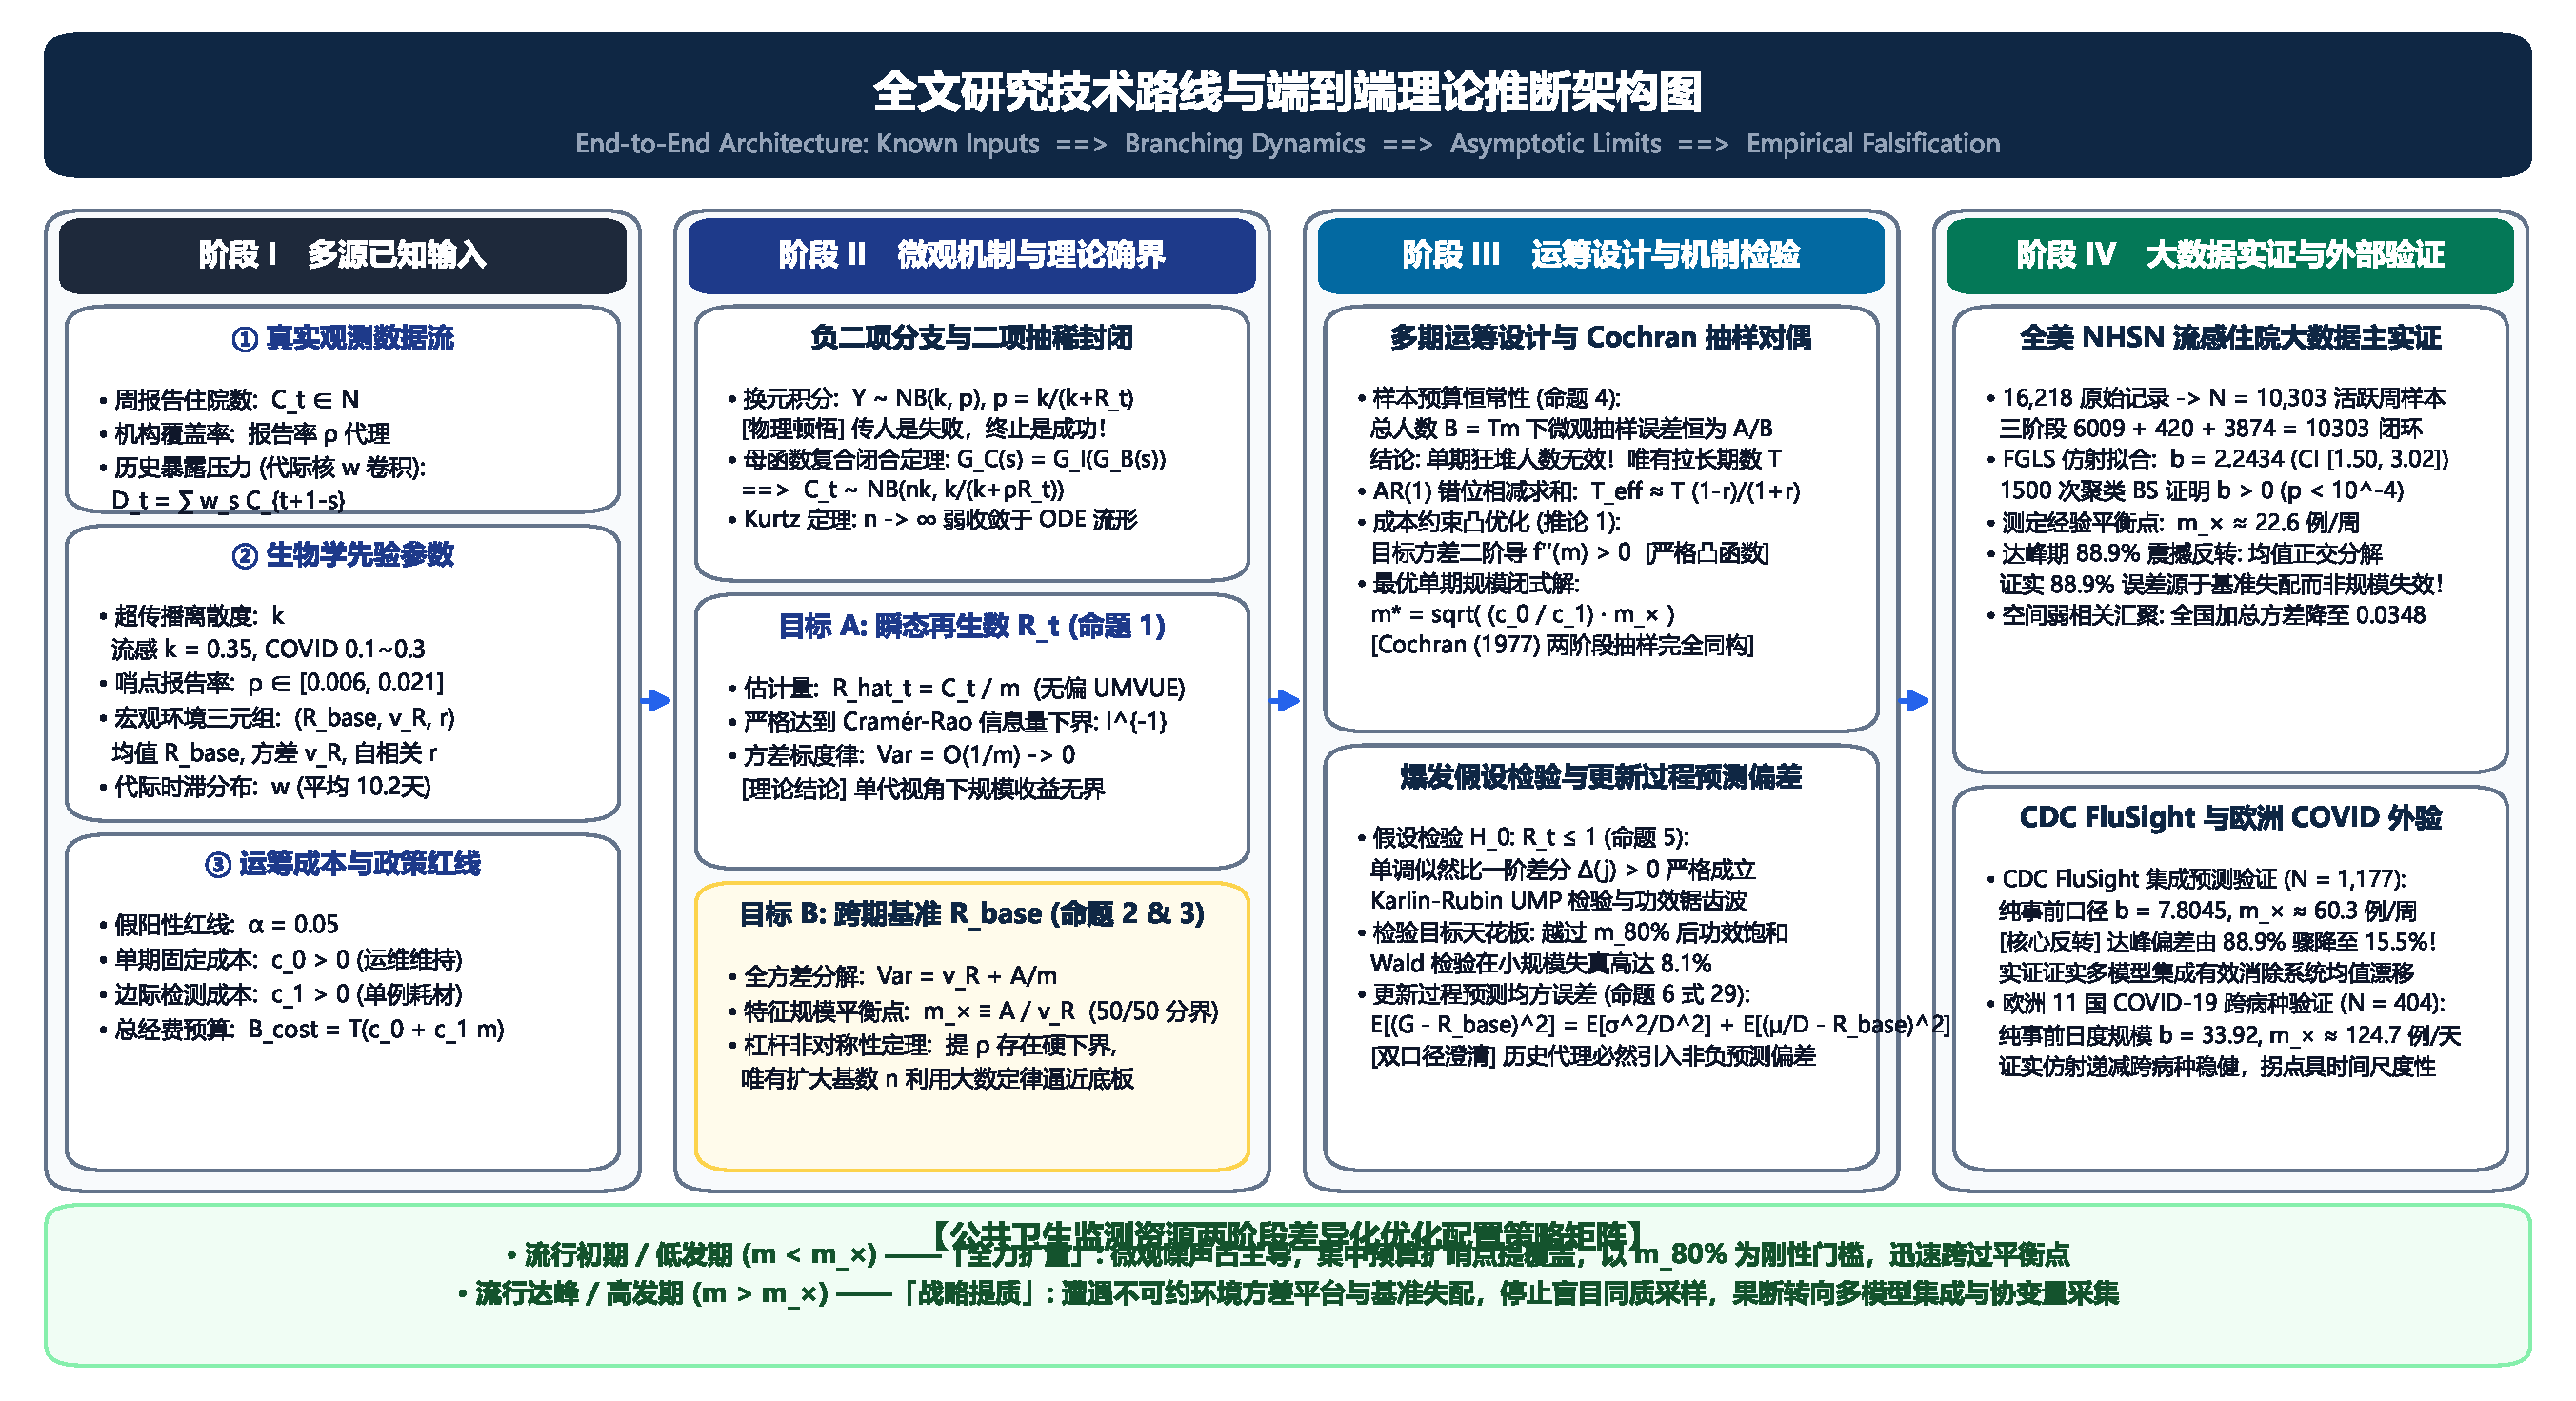
\includegraphics[width=\textwidth,height=0.38\textheight,keepaspectratio]{figures/fig0_technical_roadmap.pdf}
\caption{\textbf{全文研究技术路线与端到端理论推断全景架构图。} 展示从已知输入（真实观测数据流、生物学先验参数与运筹成本约束）到微观分支机制、渐近推断方差分解（目标 A 与目标 B 的分化）、监测运筹优化（Cochran 抽样对偶）、假设检验天花板，直至全美真实流感住院大数据计量检验与公共卫生决策矩阵的端到端逻辑闭环。}
\label{fig:technical_roadmap_ch1}
\end{figure}


本学位论文其余部分的组织架构安排如下：

\textbf{第二章：动力学建模与观测机制}。从微观生灭分支过程出发，展开个体传染力 Gamma 连续混合积分推导；深入阐释成功概率 $p = \frac{k}{k+R_t}$ 与抽稀后 $p^*$ 的统计物理顿悟；通过概率母函数复合律严格证明二项抽稀保族封闭性；并在第 2.4 节建立微观随机分支过程与宏观确定性仓室常微分方程系统的 Kurtz 流体极限动力学理论桥梁。

\textbf{第三章：渐近推断与运筹优化理论}。严格形式化定义推断目标 A 与目标 B；给出命题 1 条件似然、得分方程、双层全期望塔式法则无偏性证明与 Fisher 信息双套算法（UMVUE）；推导命题 2 跨期全方差仿射分解；证明命题 3 监测杠杆理论非对称性；给出命题 4 多期时间抽样预算恒常性与 AR(1) 错位相减求和闭式解；证明推论 1 成本优化严格凸性与 Cochran 抽样对偶。

\textbf{第四章：蒙特卡洛仿真与机制检验}。介绍 Python 蒙特卡洛随机模拟实验规格；检验命题 5 超临界增长精确检验、MLR 一阶差分、离散功效锯齿波与 Wald 正态失真；验证命题 6 更新过程单步预测两步全方差分解与式 (29) 预测偏差项；系统澄清图 1、图 2、图 3 的双口径参照关系。

\textbf{第五章：全美流感住院大数据实证分析}。详细梳理全美 CDC NHSN 监测系统背景、16,218 条原始记录筛选至 10,303 样本的客观漏斗与三大制度期算术闭环；针对重尾异方差构建 FGLS 计量拟合；汇报流行初期核心估计结果；展开达峰期 88.9\% 偏差正交分解反转；评估 2024 年自愿填报政策冲击与全国 51 辖区空间汇聚对偶收益。

\textbf{第六章：跨模型与跨病种外部扩展验证}。阐述外部验证的设计原则；汇报 CDC FluSight 官方多模型前瞻集成预测实证结果，展示多模型集成将达峰偏差压缩至 15.5\% 的去偏机制；汇报欧洲 11 国早期 COVID-19 纯事前日度发病实证结果，论证仿射递减项的跨病种普适性与经验平衡点的尺度敏感性。

\textbf{第七章：监测资源优化策略与研究展望}。构建国家公共卫生监测体系在不同流行阶段的“差异化两阶段资源配置策略矩阵”；深入剖析当前研究将平衡点作为拟合量而非测量量的方法学局限；提出基于前瞻性主动社区追踪队列的双轨解耦识别设计；对全文核心结论进行总结。

\textbf{附录 A} 提供论文所有命题与推论的保姆级中间推导展开细节。

\chapter{文献综述与理论基础}
\label{chap:lit}

本章分两部分。前一部分按六条线索梳理与研究问题直接相关的文献：再生数的定义与估计、超传播与过度离散、漏报与报告过程、估计精度的信息论刻画、环境随机性、监测设计与预测评价。每条线索都说明它为第三章的模型提供了哪个组成部分，以及它在估计目标问题上留下了什么没有回答。后一部分整理第三、四章要用到的概率与统计工具，包括分支过程与概率生成函数、负二项分布的混合表示与抽稀性质、全方差公式、信息不等式与一致最小方差无偏估计、单调似然比检验，以及两阶段抽样的方差结构。

\section{再生数的定义与估计方法}
\label{sec:lit-rt}

\subsection{基本再生数与时变再生数}

基本再生数 $R_0$ 刻画完全易感人群中一名典型感染者产生的继发感染数，是传染病动力学的核心参数\citep{anderson1991infectious, keeling2008modeling}。在异质人群中，$R_0$ 被定义为下一代算子的主特征值\citep{diekmann1990definition}，这一定义把不同类型个体之间的传播矩阵压缩为一个阈值量。流行开始后，易感者比例下降、干预措施实施、接触模式变化，传播强度随时间改变，时变再生数 $R_t$ 用于描述第 $t$ 期的实际传播水平。

再生数与可观测的增长率之间的换算依赖世代间隔分布。Wallinga 与 Lipsitch 指出，由增长率推断再生数的多种公式只在假定的世代间隔分布形状上不同，世代间隔分布的形状决定了应采用哪一个换算式\citep{wallinga2007generation}。对流感而言，家庭传播研究估计的序列间隔均值为数天：一项家庭随访研究估计为 3.6 天\citep{cowling2009estimation}，一项系统综述对季节性 H3N2 流感与 2009 年大流行流感分别估计为 2.2 天和 2.8 天\citep{vink2014serial}。这些估计都短于一周，因此在按周汇总的流感数据中，一周大致对应一代多一点的传播，按代建立的模型可以近似套用到周数据上，第五章使用的滞后权重即依此设定。

\subsection{基于更新方程的估计}

实时估计 $R_t$ 的主流方法建立在更新方程上。Wallinga 与 Teunis 用世代间隔分布把每个病例归因到可能的感染源，得到逐病例的再生数\citep{wallinga2004different}；Fraser 把更新方程写成发病数关于此前发病数的卷积，给出实时估计的框架\citep{fraser2007estimating}。Cori 等在滑动窗口内假定 $R_t$ 不变，并假设病例计数服从泊松分布，用 Gamma 共轭先验得到 $R_t$ 后验的闭式表达\citep{cori2013new}，这一方法因实现简单而被广泛使用。Thompson 等在此基础上把序列间隔的不确定性纳入估计，并区分本地病例与输入病例\citep{thompson2019improved}。Nouvellet 等给出同一框架下的简单发病预测方法\citep{nouvellet2018simple}。

方法使用中的实际问题也已有系统讨论。Gostic 等比较了多种估计方法，指出报告延迟、右删失和窗口选择会使实时估计产生偏差，并给出相应的修正建议\citep{gostic2020practical}。Abbott 等用病例与死亡数据在滚动窗口内估计全球到地方各级的时变再生数，显式处理报告延迟的不确定性，使估计基于潜在感染而非报告数\citep{abbott2020estimating}。Bettencourt 与 Ribeiro 以可观测量构建病例数的概率递推模型，对有效再生数做实时贝叶斯估计，并据此构造检验以识别异常\citep{bettencourt2008real}。窗口长度的选择也被单独研究：Parag 与 Donnelly 把 $R_t$ 写成分段常数函数，用最小描述长度原则选择分段数，避免分段过少导致的欠拟合与分段过多导致的过拟合\citep{parag2020adaptive}。半机制贝叶斯模型把更新方程、报告过程和潜在感染统一在一个层次模型中\citep{bhatt2023semi}，序贯蒙特卡洛方法则为这类模型提供了在线推断工具\citep{steyn2025primer}。大流行期间，这些框架被用于估计非药物干预的效果\citep{flaxman2020estimating}和早期传播动力学\citep{kucharski2020early}。

上述文献关注的是如何在给定数据上得到偏差小、不确定性刻画准确的 $R_t$ 估计。估计目标默认是当期 $R_t$，后验或置信区间的宽度随病例数增加而收窄。至于决策者关心跨期平均水平时误差如何随规模变化，这些文献没有单独讨论。

\section{超传播与负二项后代分布}
\label{sec:lit-superspreading}

\subsection{个体传染力的异质性}

同一种疾病的感染者之间传染力差异很大。Lloyd-Smith 等把个体再生数 $\nu$ 设为均值为 $R$、形状参数为 $k$ 的 Gamma 分布，继发感染数在给定 $\nu$ 时服从泊松分布，由此得到负二项后代分布，并在多种疾病的暴发数据上估计 $k$\citep{lloydsmith2005superspreading}。$k$ 越小，个体差异越大，少数人造成大部分传播的现象越明显。Galvani 与 May 的评论指出，个体传染性差异使超传播疾病容易引发爆发式流行，同样的波动也使暴发更容易自行熄灭\citep{galvani2005dimensions}。

在新发传染病中，离散参数 $k$ 的估计受到重视。Blumberg 与 Lloyd-Smith 用传播链规模分布同时估计 $R_0$ 与 $k$，指出 $R_0$ 的点估计只取决于平均链长，其置信区间却依赖于推断出的异质性程度\citep{blumberg2013inference}。Endo 等用中国以外地区的暴发规模估计 2019 冠状病毒病的过度离散参数，结论支持高度的传播异质性\citep{endo2020estimating}。Adam 等基于中国香港 1038 例病例的接触追踪数据估计，19\% 的病例造成了 80\% 的本地传播\citep{adam2020clustering}。

\subsection{负二项后代分布的形状}

图~\ref{fig:offspring} 用示例参数 $R=1.15$ 展示离散参数对后代分布的影响。左图为继发感染数的概率分布，纵轴取对数。$k=0.35$ 时一名感染者不产生任何继发感染的概率为 0.6009，$k=0.1$ 时升至 0.7768，同等均值下的泊松分布只有 0.3166。离散程度越高，零后代的概率越大。与泊松分布相比，负二项分布的右尾也厚得多：在 8 个继发感染处，$k=0.1$ 与 $k=0.35$ 的概率分别是泊松分布的 267 倍和 299 倍。$k=0.1$ 把更多概率放在零和更远的尾部，所以在 8 处略低于 $k=0.35$。均值相同而形状差异如此之大，说明只看平均传播强度会掩盖传播过程的随机性。

右图为传播集中度曲线。横轴是按个体再生数从高到低排序后的感染者比例，纵轴是这部分感染者贡献的期望传播份额，计算时利用了 Gamma 分布的尺寸偏倚性质，份额与 $R$ 无关。传染力最强的 20\% 感染者，在 $k=0.1$、0.35、1 时分别贡献 95.1\%、72.4\% 和 52.2\% 的传播；若所有人传染力相同，这一比例为 20\%，对应图中的对角虚线。$k=0.35$ 位于常见呼吸道传染病估计值的范围内\citep{lloydsmith2005superspreading}，这时七成以上的传播集中在两成的人身上。

\begin{figure}[!tbp]
  \centering
  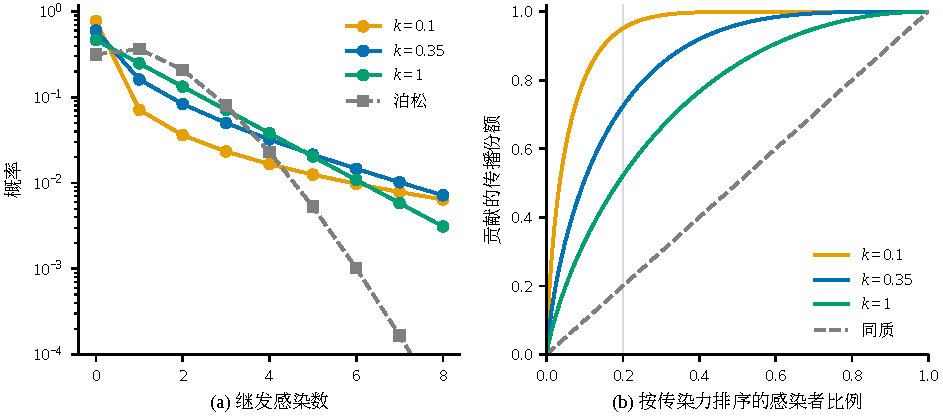
\includegraphics[width=\textwidth]{figures/fig_2_1_offspring.pdf}
  \caption{负二项后代分布与传播集中度。（a）均值 $R=1.15$ 时不同离散参数下继发感染数的概率分布，纵轴为对数刻度，虚线为同均值的泊松分布。（b）按个体再生数排序后，前一定比例感染者贡献的期望传播份额，竖线标出 20\% 处。}
  \label{fig:offspring}
\end{figure}

这种集中性对监测统计量有直接影响。一期报告病例的方差除了泊松部分 $R$ 外，还多出 $R^2/k$ 一项，第三章将看到这一项在报告完整时依然存在，只有扩大观测的感染者人数才能把它平均掉。超传播文献主要讨论 $k$ 对疫情暴发概率和防控策略的影响，较少把 $k$ 放进监测统计量的方差分解。

\subsection{分支过程理论}

负二项后代分布可以嵌入 Galton--Watson 分支过程。Harris 的专著系统建立了分支过程理论，覆盖 Galton--Watson 过程、Markov 分支过程和年龄依赖过程\citep{harris1963theory}；Athreya 与 Ney 对分支过程的极限理论作了统一处理\citep{athreya1972branching}。在流行早期，易感者耗竭可以忽略，感染者之间相互独立地产生后代，分支过程是传播的自然近似。第三章的单代模型正是一个带环境的分支过程中相邻两代之间的一步转移。

\section{漏报与报告过程}
\label{sec:lit-reporting}

\subsection{漏报的层级与规模}

监测系统记录的病例只是全部感染的一部分。Gibbons 等把漏报分为两个层级：社区中的感染者未就医，以及就医后未被报告；文献中的乘数因子在疾病和国家之间差异很大\citep{gibbons2014measuring}。Reed 等对 2009 年美国甲型 H1N1 流感的估计表明，截至当年 7 月实验室确诊的报告病例约 4.4 万例，校正漏检后实际感染估计为 180 万至 570 万例\citep{reed2009estimates}。对于住院监测，报告率可以理解为感染者中住院并被记录的比例。季节性流感的有症状侵袭率\citep{tokars2018seasonal}与住院负担\citep{zhou2012hospitalizations, rolfes2018annual}共同决定了这一比例的量级，第三章的住院情景取 0.0056 至 0.021 即由此得到。美国每个流感季的流感相关住院估计为 14 万至 71 万例\citep{rolfes2018annual}，州级周报的住院数因此在数个到数千个之间变化，为第五章检验规模效应提供了足够宽的规模范围\citep{cdc2026nhsn}。

\subsection{漏报的建模方法}

漏报对再生数估计的影响有两类处理方法。一类在估计中直接修正报告偏差：Azmon 等研究了误报数据下的再生数估计\citep{azmon2014estimating}；Stoner 等提出分层模型修正计数数据中的漏报\citep{stoner2019hierarchical}；Bracher 与 Held 用边际矩匹配方法拟合漏报数据下的地方性与流行性模型\citep{bracher2021marginal}。另一类把报告过程写成对真实计数的随机抽稀。Steutel 与 van Harn 引入的二项抽稀算子用伯努利随机变量之和代替常数乘法，保持取值为非负整数\citep{steutel1979discrete}；Al-Osh 与 Alzaid 基于这一算子提出一阶整数值自回归模型，其相关结构类似连续的一阶自回归\citep{alosh1987first}。计数回归的系统处理可见 Cameron 与 Trivedi 的专著\citep{cameron2013regression}。

二项抽稀的好处在于它与负二项分布相容：负二项变量经二项抽稀后仍服从负二项分布（见第~\ref{sec:lit-tools} 节）。这使报告病例数的条件分布有显式形式，估计量的精确性质可以写出来。报告完整与否在这种表示下只改变一个参数，报告率与覆盖面两条扩容途径的效果因而可以在同一个式子里比较。

漏报还带来测量误差问题。若用于归一化的病例规模本身含噪，回归系数会偏离真实值，这是测量误差文献中的经典结论\citep{fuller1987measurement, carroll2006measurement}。第五章解释经验斜率偏大时会用到这一点。

\section{估计精度的信息论刻画}
\label{sec:lit-information}

Fisher 信息与 Cramér--Rao 不等式是刻画估计精度上限的标准工具。Rao 给出了无偏估计量方差不低于 Fisher 信息倒数的下界\citep{rao1945information}，Cramér 在其专著中独立得到同一结果\citep{cramer1946mathematical}；现代教材把它与指数族、充分统计量和完备性联系起来\citep{casella2002statistical, lehmann1998point}。若一个无偏估计量的方差恰好等于这一下界，它在无偏估计量中是最有效的。

Parag 等把这一工具引入传染病监测。在泊松更新模型下，再生数的 Fisher 信息与窗口内的总感染压力成正比，病例越多，信息越多，估计越精确\citep{parag2022quantifying}。Parag 与 Donnelly 进一步讨论了实时推断疫情反弹的基本极限\citep{parag2022fundamental}，Parag 等又分析了带噪数据对及时干预的非对称限制：判断疫情在增长和判断疫情在下降所需的时间并不相同\citep{parag2025asymmetric}。这些结果针对的都是当期再生数，信息随病例数线性增长，与第三章的目标Ⅰ一致。

信息论方向的研究留下两处可以延伸的地方。一处是过度离散，泊松假设下信息随病例数线性增长，负二项假设下信息的表达式会多出一个与 $k$ 有关的项，需要重新推导。另一处是估计目标，若关心的量是跨期平均水平，当期 $R_t$ 围绕平均水平的波动是一项额外的误差，它不进入当期 $R_t$ 的 Fisher 信息，却决定了平均水平估计的精度上限。

\section{环境随机性}
\label{sec:lit-environment}

\subsection{生态学中的两类随机性}

种群生态学长期区分两类随机性。人口随机性来自个体出生、死亡等事件的独立随机性，环境随机性来自所有个体共同承受的外部波动。Engen 等给出了两者的严格定义：人口随机性对种群增长率方差的贡献与种群规模成反比，环境随机性的贡献不随规模变化\citep{engen1998demographic}。Lande 等的专著把这一区分作为随机种群动力学的出发点\citep{lande2003stochastic}，Bj{\o}rnstad 与 Grenfell 的综述讨论了确定性动力学、密度依赖与随机强迫的相互作用\citep{bjornstad2001noisy}。大种群中人口随机性被平均掉，种群波动主要由环境随机性驱动。

\subsection{传染病中的环境随机性}

传染病动力学同样受两类随机性共同驱动。Rohani 等分析了儿童传染病中确定性与随机性的相互作用\citep{rohani2002determinism}。Bret\'o 等提出基于机制模型的时间序列分析方法，在传播率中加入环境噪声\citep{breto2009time}；He 等用仅需模型模拟的推断方法分析麻疹数据，指出纳入超出人口随机性的额外噪声对处理环境随机性和模型误设很重要\citep{he2010plug}。Rasmussen 等结合基因谱系与时间序列推断随机环境下的传播参数\citep{rasmussen2011inference}。

流感传播的环境驱动因素已有较多实证证据。Shaman 与 Kohn 重新分析实验数据，发现绝对湿度解释了 50\% 的流感病毒传播变异和 90\% 的病毒存活变异\citep{shaman2009absolute}；Shaman 等进一步发现美国流感季的起始与此前数周绝对湿度异常偏低相关，用观测湿度调节传播率即可复现流感的季节周期\citep{shaman2010absolute}。Dalziel 等表明城市化程度与湿度共同塑造美国城市流感流行的强度\citep{dalziel2018urbanization}。这些研究说明，同一辖区同一时期的感染者共享随时间变化的环境，各期 $R_t$ 围绕平均水平的波动有实在的物理与社会来源。

生态学的两类随机性区分尚未被系统地用于监测统计量的精度分析。环境波动在生态学中决定种群灭绝风险，在监测问题中则决定跨期平均水平估计的精度底板。把两者对应起来，需要在监测数据的生成机制中显式写出环境层，并说明观测规模与人口随机性部分的关系。

\section{监测设计与抽样理论}
\label{sec:lit-design}

\subsection{监测系统的设计与评价}

监测系统的设计长期依赖经验规则和定性评价。美国疾病控制与预防中心发布的监测系统评价指南从有用性、简单性、灵活性、数据质量、灵敏度、代表性和及时性等方面评价监测系统\citep{german2001updated}，但没有给出规模与精度之间的定量关系。哨点选址研究给出了一些定量证据：Polgreen 等用最大覆盖模型为美国爱荷华州的流感哨点选址，发现新增站点的人口覆盖呈边际收益递减，10 个优化站点即可达到现有 22 个站点的覆盖率\citep{polgreen2009optimizing}。Scarpino 等利用历史监测数据优化得克萨斯州的哨点招募，优化后的网络用较少的哨点就能优于现有网络，原因在于避免了信息冗余\citep{scarpino2012optimizing}。

这些研究的优化目标是人口覆盖率或与参考序列的拟合程度，收益递减来自站点之间的信息重叠。规模收益递减还有一个来源，即环境项不随规模下降，监测设计文献很少从估计方差的结构推出环境底板。

\subsection{两阶段抽样与方差分量}

抽样调查理论为讨论规模收益提供了现成框架。两阶段抽样先抽初级单元，再在每个初级单元内抽次级单元，估计量的方差由初级单元间方差和初级单元内方差两部分组成，前者只能通过增加初级单元数来降低\citep{cochran1977sampling}。Cochran 给出了在线性费用函数下初级单元内最优样本量的公式，Kish 提出的设计效应把整群抽样的方差膨胀归结为组内相关\citep{kish1965survey}，Lohr 的现代教材对这些结果作了系统整理\citep{lohr2022sampling}。方差分量的估计方法可见 Searle 等的专著\citep{searle1992variance}。

监测问题与两阶段抽样在结构上相似。各观测期可以看作初级单元，环境方差对应初级单元间方差，人口随机性与报告过程对应初级单元内方差。两者的差别在于独立性：抽样调查中初级单元按设计独立抽取，监测数据中的各期环境可能存在时间相关，次级单元的数目也由此前的传播产生。第四章讨论的正是这种对应能延伸多远。时间相关的处理需要平稳过程部分和的方差公式\citep{hamilton1994time}。

\section{离散分布下的假设检验}
\label{sec:lit-testing}

判断疫情是否在增长，在统计上是一个单侧检验问题。对单参数指数族，单调似然比性质保证了单侧检验存在一致最优解，这就是 Karlin--Rubin 定理\citep{karlin1956theory, lehmann2005testing}。离散分布下，非随机化检验通常无法恰好达到名义水平，实际水平小于等于名义水平。

常用的 Wald 近似检验在小样本下的表现并不可靠。Brown 等对二项比例的研究表明，标准 Wald 区间的覆盖概率随样本量呈持续的不规则振荡，教科书中常用的安全条件并不能保证覆盖\citep{brown2001interval}；Agresti 与 Coull 发现反转得分检验得到的区间即使在样本很小时也接近名义水平\citep{agresti1998approximate}。这些结论针对二项分布，负二项计数在规模较小、离散程度较高时偏离正态更明显，Wald 检验可能出现类似甚至更严重的问题。第四章对此给出具体计算。

\section{预测评价}
\label{sec:lit-forecast}

近年来传染病预测的评价体系逐步完善。Reich 等比较了美国季节性流感的实时多模型集成预测，发现集成预测的准确度通常优于大多数单个模型\citep{reich2019accuracy}。Cramer 等评价了美国 2019 冠状病毒病死亡人数的个体与集成概率预测\citep{cramer2022evaluation}。Mathis 等评价了 2021--2022 和 2022--2023 两个流感季的美国流感前瞻预测项目，该项目以州级流感住院数为预测对象\citep{mathis2024evaluation}。在评分方法上，Bracher 等说明了如何用加权区间评分评价以分位数形式发布的预测\citep{bracher2021evaluating}，Bosse 等讨论了在对数等变换尺度上评分的好处，变换后的评分更接近相对误差\citep{bosse2023scoring}。

预测评价文献报告了误差随时间和地区的变化，较少把误差与预测对象的规模联系起来。若误差含有不随规模下降的成分，按相对误差排序时，大规模地区和流行高峰期的表现会系统地差于理论上的泊松预期。第六章用集成预测检验这一点。

\section{研究述评}
\label{sec:lit-review}

表~\ref{tab:lit-lines} 把上述六条文献线索与本研究的衔接归纳在一起。各条线索为模型提供了不同的组成部分。更新方程文献提供估计框架，超传播文献提供后代分布，漏报文献提供报告过程。信息论文献提供精度刻画的工具，环境随机性文献提供两类随机性的区分，抽样理论提供方差分解与费用分配的范式。

\begin{table}[!tbp]
  \centering
  \caption{文献线索与本研究的衔接}
  \label{tab:lit-lines}
  \small
  \begin{tabularx}{\textwidth}{@{}p{2.2cm}p{3.0cm}XX@{}}
    \toprule
    文献线索 & 代表文献 & 已有工作的重点 & 本研究借用与延伸之处 \\
    \midrule
    更新方程与 $R_t$ 估计 & \citet{cori2013new}；\citet{gostic2020practical} & 当期 $R_t$ 的实时估计、延迟与窗口选择 & 区分当期与跨期两个估计目标 \\
    超传播 & \citet{lloydsmith2005superspreading}；\citet{endo2020estimating} & 离散参数 $k$ 的估计与暴发风险 & 把 $R^2/k$ 写入监测统计量的方差 \\
    漏报与报告过程 & \citet{gibbons2014measuring}；\citet{steutel1979discrete} & 漏报乘数与报告偏差修正 & 用二项抽稀得到报告数的精确分布 \\
    信息论 & \citet{parag2022quantifying}；\citet{parag2025asymmetric} & 泊松模型下信息随病例数增长 & 推广到负二项并加入环境层 \\
    环境随机性 & \citet{engen1998demographic}；\citet{shaman2010absolute} & 两类随机性的定义与环境驱动证据 & 环境方差成为估计精度的底板 \\
    监测设计与抽样 & \citet{cochran1977sampling}；\citet{polgreen2009optimizing} & 两阶段费用分配、哨点覆盖 & 成本最优单期规模及其时间相关修正 \\
    \bottomrule
  \end{tabularx}
\end{table}

综合起来，现有研究在三个方面留有余地。估计目标方面，再生数估计与信息论文献默认目标是当期 $R_t$，没有讨论跨期平均水平的估计误差为何会在规模扩大后趋平。随机性来源方面，生态学对两类随机性的区分很成熟，传染病文献也承认环境驱动，二者之间缺少一个把环境方差折算成病例数的刻度。设计方面，监测系统评价以定性指标为主，哨点优化研究以覆盖率为目标，抽样理论的费用分配结论没有被系统地移植到监测问题上，移植时独立性假设是否成立也未见讨论。第三章用一个包含环境层、负二项传播和二项报告的模型回应前两点，第四章回应第三点。

\section{理论基础}
\label{sec:lit-tools}

本节整理后文推导所需的概率与统计工具。证明从略的结论都是教材中的标准结果，引用处给出出处。

\subsection{分支过程与概率生成函数}

取值于非负整数的随机变量 $X$ 的概率生成函数定义为 $G_X(s)=\E(s^X)$，$|s|\le1$。它唯一决定 $X$ 的分布，且 $\E X=G_X'(1)$，$\Var X=G_X''(1)+G_X'(1)-G_X'(1)^2$。若 $X_1,\dots,X_n$ 独立同分布，其和的概率生成函数为 $G_X(s)^n$。若 $N$ 与 $\{X_i\}$ 独立，随机和 $\sum_{i=1}^N X_i$ 的概率生成函数为复合函数 $G_N(G_X(s))$。

Galton--Watson 分支过程中，第 $g$ 代的每个个体独立地按同一后代分布产生下一代个体\citep{harris1963theory, athreya1972branching}。若第 $g$ 代有 $n$ 个个体，后代分布的概率生成函数为 $G(s)$，则第 $g+1$ 代个体数的概率生成函数为 $G(s)^n$。第三章的单代模型就是在给定 $n$ 和环境的条件下考察这一步转移。

\subsection{负二项分布的混合表示与可加性}

记 $\NB(k,p)$ 为形状参数 $k>0$、成功概率 $p\in(0,1)$ 的负二项分布，概率质量函数为
\begin{equation}
  \Pr(X=x)=\frac{\Gamma(x+k)}{\Gamma(k)\,x!}\,p^{k}(1-p)^{x},\qquad x=0,1,2,\dots
  \label{eq:nb-pmf}
\end{equation}
其概率生成函数为 $G(s)=\{p/[1-(1-p)s]\}^{k}$。取 $p=k/(k+R)$，均值为 $R$，方差为 $R+R^2/k$。

这一分布可以由泊松--Gamma 混合得到。若 $\nu\sim\mathrm{Gamma}$，形状参数为 $k$、均值为 $R$，在给定 $\nu$ 时 $X\sim\mathrm{Poisson}(\nu)$，则 $X$ 的边际分布为 $\NB(k,k/(k+R))$\citep{lloydsmith2005superspreading, cameron2013regression}。方差中的 $R$ 来自泊松部分，$R^2/k$ 来自个体再生数 $\nu$ 的方差，后者正是超传播的来源。

由概率生成函数的乘积性质，$n$ 个独立的 $\NB(k,p)$ 之和服从 $\NB(nk,p)$。形状参数相加、成功概率不变，这一可加性使一代感染者的后代总数仍为负二项分布。

\subsection{二项抽稀}

设 $I$ 为非负整数随机变量，给定 $I$ 时 $C\mid I\sim\Bin(I,\rho)$，称 $C$ 为 $I$ 以概率 $\rho$ 抽稀的结果\citep{steutel1979discrete}。由随机和的复合公式，抽稀后的概率生成函数为
\begin{equation}
  G_C(s)=G_I(1-\rho+\rho s).
  \label{eq:thinning-pgf}
\end{equation}
若 $I\sim\NB(K,p)$，代入得 $G_C(s)=\{p'/[1-(1-p')s]\}^{K}$，其中 $p'=p/[p+\rho(1-p)]$，即 $C\sim\NB(K,p')$。负二项分布对二项抽稀封闭：形状参数不变，均值乘以 $\rho$。这一性质是第三章推导报告病例数精确分布的关键。

\subsection{全方差公式}

对任意随机变量 $Y$ 与条件变量 $Z$，若方差存在，则有如下分解：
\begin{equation}
  \Var(Y)=\E[\Var(Y\mid Z)]+\Var[\E(Y\mid Z)].
  \label{eq:total-variance}
\end{equation}
右端第一项为条件方差的期望，第二项为条件期望的方差。在两阶段抽样中，前者对应初级单元内的方差，后者对应初级单元间的方差\citep{cochran1977sampling, searle1992variance}。第三章取 $Z=R_t$，前者随观测规模下降，后者等于环境方差，不随规模变化。

\subsection{信息不等式与一致最小方差无偏估计}

设样本 $X$ 的分布族 $\{f(x;\theta)\}$ 满足通常的正则条件，记得分函数与 Fisher 信息为
\begin{equation*}
  S(\theta)=\frac{\partial\log f(X;\theta)}{\partial\theta},\qquad \mathcal{I}(\theta)=\Var[S(\theta)].
\end{equation*}
对 $\theta$ 的任一无偏估计量 $T$，有 Cramér--Rao 不等式\citep{rao1945information, cramer1946mathematical}
\begin{equation}
  \Var(T)\ge \mathcal{I}(\theta)^{-1}.
  \label{eq:crlb}
\end{equation}
等号成立的充要条件是得分函数可以写成 $S(\theta)=a(\theta)[T-\theta]$ 的形式，且此时 $a(\theta)=\mathcal{I}(\theta)$\citep{casella2002statistical}。这一条件给出了判断估计量是否达到下界的简便方法：只要把得分函数整理成估计误差的倍数即可。

若 $T$ 是完备充分统计量的函数且无偏，由 Lehmann--Scheff\'e 定理，$T$ 是唯一的一致最小方差无偏估计\citep{lehmann1998point}。对单参数指数族，自然充分统计量在参数空间含开区间时是完备的。负二项分布在形状参数已知时属于这一类。

\subsection{单调似然比与一致最优检验}

若对任意 $\theta_1<\theta_2$，似然比 $f(x;\theta_2)/f(x;\theta_1)$ 是统计量 $T(x)$ 的非减函数，称分布族关于 $T$ 具有单调似然比。对这样的分布族，检验 $H_0:\theta\le\theta_0$ 对 $H_1:\theta>\theta_0$ 时，拒绝域形如 $\{T>c\}$ 的检验在其水平下是一致最优的\citep{karlin1956theory, lehmann2005testing}。离散分布下若不采用随机化，临界值 $c$ 只能取使实际水平不超过名义水平的最小整数，实际水平 $\alpha^*\le\alpha$，且随样本量非单调变化。第四章构造的精确增长检验即属此类。

\subsection{两阶段抽样的方差与费用最优分配}

设总体由若干初级单元组成，初级单元间方差为 $S_b^2$，单元内方差为 $S_w^2$。抽 $T$ 个初级单元、每个单元内抽 $m$ 个次级单元，样本均值的方差在忽略有限总体校正时近似为
\begin{equation}
  \Var(\bar{y})\approx\frac{S_b^2}{T}+\frac{S_w^2}{Tm}.
  \label{eq:two-stage}
\end{equation}
若总费用为 $T(c_1'+c_2'm)$，其中 $c_1'$ 为每个初级单元的固定费用，$c_2'$ 为每个次级单元的费用，则在固定总费用下使方差最小的单元内样本量为
\begin{equation}
  m^{\mathrm{opt}}=\sqrt{\frac{c_1'}{c_2'}\cdot\frac{S_w^2}{S_b^2}}.
  \label{eq:cochran-opt}
\end{equation}
式~\eqref{eq:cochran-opt} 见于 Cochran 的第十章\citep{cochran1977sampling}。它表明单元内样本量只取决于费用比与方差比，与总预算无关。第四章将看到，监测问题中的成本最优单期规模具有完全相同的形式。

\chapter{模型与两个估计目标}
\label{chap:model}

第二章的综述把研究缺口归结为两点：当期再生数之外的估计目标缺少误差分析，环境方差缺少一把折算成病例数的尺子。本章建立一个包含环境层、负二项传播与二项报告的单代模型，在四条明确假设下推导两个估计目标的有限样本方差。第~\ref{sec:model-setup}~节给出模型与报告病例数的精确分布；第~\ref{sec:model-targets}~节定义两个估计目标并列出基本假设；第~\ref{sec:model-current}~节讨论当期再生数的估计；第~\ref{sec:model-average}~节推导跨期平均水平的方差并定义交叉点；第~\ref{sec:model-reporting}~节比较报告率与覆盖面两条扩容途径。各命题的完整证明放在附录~A，正文给出推导思路与直觉。

\section{传播与报告的两层模型}
\label{sec:model-setup}

\subsection{模型设定}

考虑第 $t$ 期的传播。上一代有 $n$ 名感染者，第 $i$ 人产生 $X_{i,t}$ 个继发感染。为刻画超传播，设给定当期再生数 $R_t$ 时 $X_{i,t}$ 相互独立，服从负二项分布
\begin{equation}
  X_{i,t}\mid R_t \sim \NB\Bigl(k,\ \frac{k}{k+R_t}\Bigr),\qquad
  \E(X_{i,t}\mid R_t)=R_t,\quad \Var(X_{i,t}\mid R_t)=R_t+\frac{R_t^2}{k}.
  \label{eq:offspring}
\end{equation}
这里 $k$ 是离散参数。由第~\ref{sec:lit-tools}~节的混合表示，式~\eqref{eq:offspring} 等价于个体再生数服从均值为 $R_t$、形状参数为 $k$ 的 Gamma 分布，继发感染数在其上服从泊松分布\citep{lloydsmith2005superspreading}。方差中的 $R_t$ 是泊松部分，$R_t^2/k$ 是个体传染力差异带来的部分，$k$ 越小这一部分越大。

同期新感染总数 $I_t=\sum_{i=1}^{n}X_{i,t}$。由负二项分布的可加性，$I_t\mid R_t\sim\NB(nk,\,k/(k+R_t))$。监测系统只看到其中一部分，每名新感染者独立地以概率 $\rho$ 被报告，报告病例数 $C_t\mid I_t\sim\Bin(I_t,\rho)$。图~\ref{fig:mechanism} 示意了这一过程：顶部的环境层表示同一期所有感染者共享同一个 $R_t$。左栏的 $n$ 名感染者经负二项传播产生数目差别很大的新感染者，其中一人产生 7 个，体现超传播；右栏的二项抽稀让每名新感染者独立地以概率 $\rho$ 进入监测数据，图中 11 名新感染者里有 3 名被报告。监测系统只能看到最终的报告数 $C_t$，传播与报告两层随机性都包含在其中。

\begin{figure}[!tbp]
  \centering
  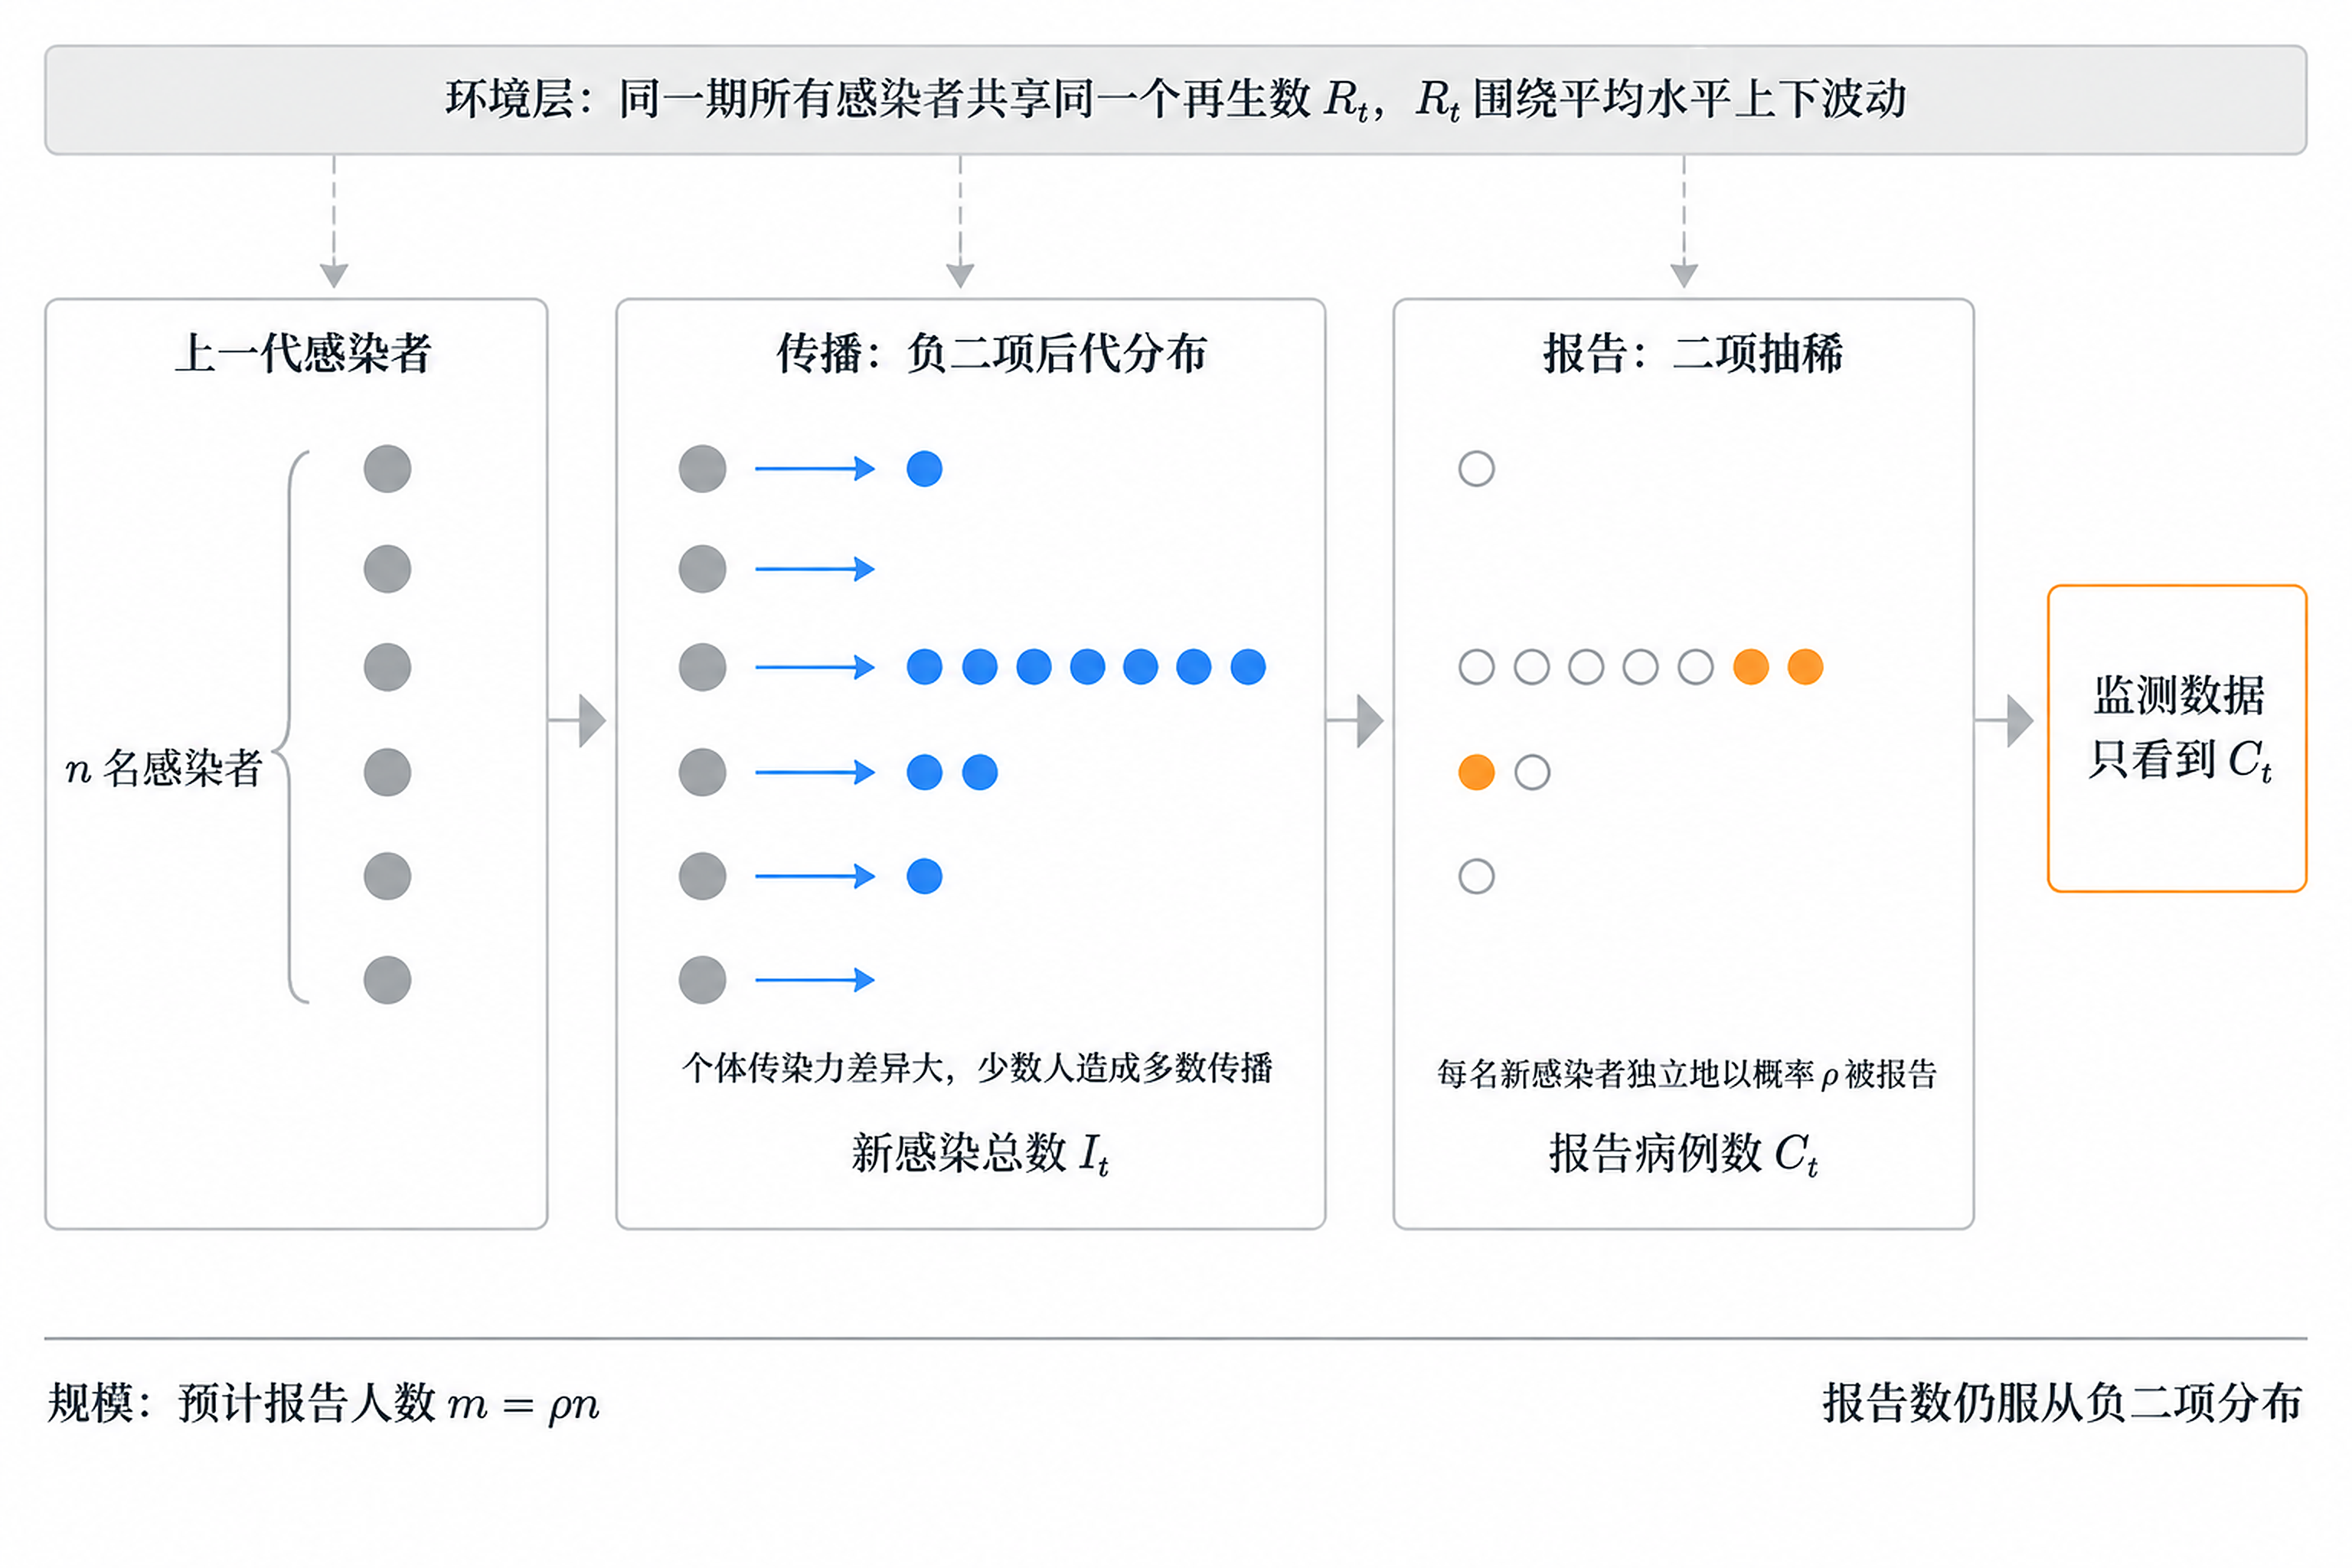
\includegraphics[width=\textwidth]{figures/fig_3_1_mechanism.png}
  \caption{传播与报告的两层模型示意。环境层决定当期再生数 $R_t$，上一代 $n$ 名感染者按负二项后代分布产生新感染者，新感染者再经二项抽稀成为报告病例；监测数据只记录报告病例数 $C_t$。}
  \label{fig:mechanism}
\end{figure}

\subsection{报告病例数的精确分布}

由第~\ref{sec:lit-tools}~节的抽稀封闭性，把 $I_t$ 的分布代入式~\eqref{eq:thinning-pgf}，得到报告病例数的条件分布
\begin{equation}
  \begin{gathered}
  C_t\mid n, R_t \sim \NB\Bigl(nk,\ \frac{k}{k+\rho R_t}\Bigr),\\
  \E(C_t\mid n,R_t)=\rho n R_t,\qquad
  \Var(C_t\mid n,R_t)=\rho n R_t+\frac{\rho^2 n R_t^2}{k}.
  \end{gathered}
  \label{eq:report-dist}
\end{equation}
推导只需一步。$I_t$ 的概率生成函数为 $\{k/(k+R_t-R_t s)\}^{nk}$，以 $1-\rho+\rho s$ 代 $s$，分母变为 $k+\rho R_t-\rho R_t s$，形状参数 $nk$ 不变，$R_t$ 被替换为 $\rho R_t$。所以报告过程相当于把再生数打了一个 $\rho$ 折扣，分布族不变。

记 $m=\rho n$，即上一代感染者中预计被报告的人数，下文用 $m$ 度量监测规模。$m$ 同时依赖覆盖的感染者人数 $n$ 和报告率 $\rho$。在住院监测中，$n$ 可以理解为辖区内上一代的全部感染者，$\rho$ 为感染者中住院并被记录的比例，$m$ 则近似等于上一周的报告住院数。

报告数的相对方差可以写成两项之和：
\begin{equation}
  \frac{\Var(C_t\mid n,R_t)}{\E(C_t\mid n,R_t)^2}=\frac{1}{\rho n R_t}+\frac{1}{nk}.
  \label{eq:relvar}
\end{equation}
第一项来自报告抽样，与预计报告数 $\rho nR_t$ 成反比，提高报告率可以压低它；第二项来自超传播，只与感染者人数 $n$ 和离散参数 $k$ 有关，与报告率无关。报告率再高，第二项也不会消失，因为它描述的是传播本身的随机性，与观测是否完整无关。这一不对称在第~\ref{sec:model-reporting}~节会以命题的形式再次出现。

\section{两个估计目标与基本假设}
\label{sec:model-targets}

\subsection{估计目标的区分}

$R_t$ 随时间波动。天气、学校假期和人群流动让各期的传播强度围绕某个平均水平上下变化，第二章列举的湿度与城市化证据\citep{shaman2010absolute, dalziel2018urbanization}说明这种波动有实在的来源。设 $\E(R_t)=\Rbar$，$\Var(R_t)=v_R$，称 $v_R$ 为环境方差。

监测要回答的问题可以分为两类。目标Ⅰ是当期再生数 $R_t$。例如卫生部门想知道本周的传播是否比上周更快，或者某项干预实施后传播是否减弱，关心的是这一期实际发生的 $R_t$。目标Ⅱ是平均水平 $\Rbar$。例如为一个流行季制定床位计划，或比较不同季节的典型传播强度，需要的是该时段有代表性的传播水平，单期的 $R_t$ 只是围绕 $\Rbar$ 的一次随机实现。

两个目标使用同一个估计量 $\widehat R_t=C_t/(\rho n)$，误差的参照对象不同。目标Ⅰ的误差是 $\widehat R_t-R_t$，目标Ⅱ的误差是
\begin{equation}
  \widehat R_t-\Rbar=(\widehat R_t-R_t)+(R_t-\Rbar).
  \label{eq:error-split}
\end{equation}
右端第一项是测量误差，随规模缩小；第二项是环境偏离，与规模无关。目标Ⅱ因此比目标Ⅰ多出一个不随规模变化的误差来源。这一分解是全章的出发点，后面的命题都是对它的定量刻画。

\subsection{基本假设}

本章与第四章的推导依赖以下四条假设。

\begin{enumerate}[label=H\arabic*]
  \item 给定 $R_t$，各感染者的继发感染数相互独立且服从式~\eqref{eq:offspring}，报告过程为独立二项抽样。
  \item 同一期的感染者共享同一个 $R_t$，即环境扰动作用在“期”这一层面。
  \item 离散参数 $k$ 与报告率 $\rho$ 已知。
  \item 规模 $n$ 与当期环境无关：$\E(R_t\mid n)=\Rbar$，$\Var(R_t\mid n)=v_R$。
\end{enumerate}

H1 是分支过程的标准假设，在流行早期易感者耗竭可以忽略时较为合理。它排除了感染者之间的相互影响，例如同一家庭内多名感染者共同传播给同一个人。H2 把环境波动放在期的层面，同一期内所有感染者面对同一个传播强度。若同一期内不同亚群面对不同环境，H2 可以放宽为多个环境的汇总，见第~\ref{sec:model-pooling}~节。

H3 在实践中只是近似。$k$ 需要从接触追踪或暴发规模数据中估计\citep{lloydsmith2005superspreading, endo2020estimating}，$\rho$ 需要从血清学调查或负担估计中推算\citep{reed2009estimates, tokars2018seasonal}。$k$ 与 $\rho$ 未知时，估计量的形式不变，方差中会多出参数不确定性的贡献，第四章讨论增长检验时会说明 $k$ 设定偏差的影响。

H4 需要单独说明。若 $n$ 由设计固定，例如每期追踪固定数目的指示病例，H4 自然成立。若 $n_t$ 是此前传播的结果，而 $R_t$ 又有时间相关，那么大的 $n_t$ 往往出现在 $R$ 偏高的时期，H4 不再自动成立。真实监测序列属于后一种情况，规模本身是随机的，第~\ref{sec:design-renewal}~节专门用更新过程的模拟讨论随机规模的影响。

本章其余部分使用的主要符号汇总于表~\ref{tab:symbols}。

\begin{table}[!tbp]
  \centering
  \caption{主要符号}
  \label{tab:symbols}
  \small
  \begin{tabularx}{\textwidth}{@{}lX@{}}
    \toprule
    符号 & 含义 \\
    \midrule
    $R_t$ & 第 $t$ 期的当期再生数，目标Ⅰ \\
    $\Rbar$，$v_R$ & 当期再生数的跨期平均水平与环境方差，$\Rbar$ 为目标Ⅱ \\
    $k$ & 负二项后代分布的离散参数，越小表示超传播越明显 \\
    $n$ & 上一代感染者人数 \\
    $\rho$ & 每名新感染者被报告的概率 \\
    $m=\rho n$ & 预计报告规模，即上一代感染者中预计被报告的人数 \\
    $I_t$，$C_t$ & 第 $t$ 期新感染总数与报告病例数 \\
    $\widehat R_t=C_t/(\rho n)$ & 两个目标共用的估计量 \\
    $A=\Rbar+\rho(\Rbar^2+v_R)/k$ & 规模项系数 \\
    $V(m)=v_R+A/m$ & 目标Ⅱ的估计方差 \\
    $\mx=A/v_R$ & 交叉点，规模项与环境项相等时的预计报告规模 \\
    $\mathcal{I}(R_t)$ & 报告病例数关于 $R_t$ 的 Fisher 信息 \\
    \bottomrule
  \end{tabularx}
\end{table}

\section{当期再生数的估计}
\label{sec:model-current}

先看目标Ⅰ。此时 $R_t$ 视为固定参数，估计量的性质由式~\eqref{eq:report-dist} 直接决定。

\begin{proposition}[当期再生数的有效估计]
\label{prop:current}
在 H1--H3 下，给定 $n$ 与 $R_t>0$，估计量 $\widehat R_t=C_t/(\rho n)$ 满足：
\begin{enumerate}[label=(\roman*)]
  \item $\widehat R_t$ 是 $R_t$ 的极大似然估计；当 $C_t=0$ 时，似然在边界 $R_t=0$ 处取最大值；
  \item $\widehat R_t$ 无偏，方差为 $\Var(\widehat R_t\mid n,R_t)=R_t/(\rho n)+R_t^2/(kn)$；
  \item 对任意 $n$，该方差都等于 Cramér--Rao 下界 $1/\mathcal I(R_t)$，其中 $\mathcal I(R_t)=n/(R_t/\rho+R_t^2/k)$；
  \item $\widehat R_t$ 是 $R_t$ 的一致最小方差无偏估计。
\end{enumerate}
\end{proposition}

推导的核心是把对数似然对 $R_t$ 求导。略去与 $R_t$ 无关的常数，由式~\eqref{eq:nb-pmf} 与式~\eqref{eq:report-dist}，对数似然为
\begin{equation}
  \ell(R_t)=C_t\log R_t-(nk+C_t)\log(k+\rho R_t).
  \label{eq:loglik}
\end{equation}
对 $R_t$ 求导并通分，分子中含 $C_t\rho R_t$ 的两项相互抵消，得到
\begin{equation}
  S(R_t)=\frac{C_t}{R_t}-\frac{\rho(nk+C_t)}{k+\rho R_t}
  =\frac{k\,(C_t-\rho nR_t)}{R_t(k+\rho R_t)}
  =\mathcal{I}(R_t)\,(\widehat R_t-R_t),
  \label{eq:score}
\end{equation}
其中 $\mathcal{I}(R_t)=k\rho n/[R_t(k+\rho R_t)]=n/(R_t/\rho+R_t^2/k)$。四条结论都可以从这个式子读出。令 $S=0$ 得到 $\widehat R_t$，这是结论 (i)；若 $C_t=0$，$\ell(R_t)=-nk\log(k+\rho R_t)$ 在 $R_t\ge0$ 上单调递减，最大值落在边界 0。由式~\eqref{eq:report-dist}，$\E\widehat R_t=R_t$，方差为 $\Var(C_t)/(\rho n)^2$，化简即得结论 (ii)。得分函数恰好是估计误差的 $\mathcal{I}(R_t)$ 倍，满足第~\ref{sec:lit-tools}~节所述 Cramér--Rao 等号成立的条件，因此方差等于 $1/\mathcal{I}(R_t)$，这是结论 (iii)。

结论 (iii) 不是渐近结果。通常极大似然估计只在样本量趋于无穷时才渐近达到下界，这里在每个有限 $n$ 处都精确达到。原因是负二项分布在 $k$ 已知时是以 $C_t$ 为充分统计量的单参数指数族，而 $\widehat R_t$ 恰好是充分统计量的线性函数。结论 (iv) 来自同一事实，即 $C_t$ 是完备充分统计量，$\widehat R_t$ 是它的无偏函数，由 Lehmann--Scheff\'e 定理即为一致最小方差无偏估计\citep{lehmann1998point, casella2002statistical}。精确达到下界需要 $k$ 已知；$k$ 未知时，模型变为两参数，$C_t$ 不再是完备充分统计量。

方差的两部分与式~\eqref{eq:relvar} 一一对应，$R_t/(\rho n)$ 来自报告抽样，$R_t^2/(kn)$ 来自超传播。两部分都按 $1/n$ 衰减，规模越大，当期再生数估得越准，没有底板。Parag 等在泊松更新模型下发现信息与病例数成正比\citep{parag2022quantifying}，命题~\ref{prop:current} 是信息正比于病例数在负二项与漏报下的精确形式，在 $k\to\infty$ 且 $\rho=1$ 时，$\mathcal{I}(R_t)=n/R_t$，回到泊松情形。超传播使信息打了折扣，$k$ 越小折扣越大。

为核对结论 (iii)，在 $m$ 从 1 到 1000 的 10 个规模上各做 20,000 次模拟，方差与 Cramér--Rao 下界之比在 0.98--1.02，差异在蒙特卡洛误差范围内（图~\ref{fig:variance}a 中的圆点）。

\section{跨期平均水平与交叉点}
\label{sec:model-average}

\subsection{方差结构}

目标Ⅱ要估计的是 $\Rbar$。此时 $R_t$ 是随机的，估计误差多出了式~\eqref{eq:error-split} 中的环境偏离项。

\begin{proposition}[跨期平均水平的方差]
\label{prop:average}
在 H1--H4 下，$\widehat R_t=C_t/(\rho n)$ 是 $\Rbar$ 的无偏估计，其方差为
\begin{equation}
  V(m)=\Var(\widehat R_t\mid n)=v_R+\frac{\Rbar}{\rho n}+\frac{\Rbar^2+v_R}{kn}
  =v_R+\frac{A}{m},\qquad A=\Rbar+\frac{\rho(\Rbar^2+v_R)}{k}.
  \label{eq:var-average}
\end{equation}
定义交叉点 $\mx=A/v_R$，则：
\begin{enumerate}[label=(\roman*)]
  \item $m\to\infty$ 时 $V(m)\to v_R$；
  \item 规模项在总方差中的份额为 $1/(1+m/\mx)$，在 $m=\mx$ 处两项各占一半；
  \item 规模从 $m$ 翻倍到 $2m$，方差下降的比例为 $1/[2(1+m/\mx)]$；
  \item $V(m)$ 严格递减且严格凸，对 $m$ 的弹性为 $-\mx/(m+\mx)$，在 $m=\mx$ 处等于 $-1/2$。
\end{enumerate}
\end{proposition}

式~\eqref{eq:var-average} 由全方差公式~\eqref{eq:total-variance} 得到，取条件变量为 $R_t$。由 H4，条件于 $n$ 时 $R_t$ 的均值与方差仍为 $\Rbar$ 与 $v_R$。条件均值 $\E(\widehat R_t\mid R_t)=R_t$，它的方差就是环境方差 $v_R$；条件方差由命题~\ref{prop:current}(ii) 给出，对 $R_t$ 取期望时，$R_t$ 的一次项变为 $\Rbar$，二次项变为 $\E(R_t^2)=\Rbar^2+v_R$，于是得到 $\Rbar/(\rho n)+(\Rbar^2+v_R)/(kn)$。把 $n=m/\rho$ 代入，两项合并为 $A/m$。$A$ 中出现 $\Rbar^2+v_R$ 而非 $\Rbar^2$，是因为超传播项与 $R_t$ 的平方成正比，环境波动让平方的期望变大。

四条结论都是 $V(m)=v_R+A/m$ 的初等推论。规模项份额为 $(A/m)/(v_R+A/m)$，分子分母同除以 $A/m$ 即得 $1/(1+m/\mx)$。翻倍降幅为 $[V(m)-V(2m)]/V(m)=(A/2m)/(v_R+A/m)$，正是份额的一半。弹性为 $V'(m)\,m/V(m)=-(A/m)/(v_R+A/m)$，即份额的相反数。二阶导数 $V''(m)=2A/m^3>0$，所以 $V$ 严格凸。这几个量的共同点是都只依赖比值 $m/\mx$：交叉点把不同参数下的方差曲线统一到同一把尺子上，规模达到交叉点的几倍，就可以直接读出规模项还剩多少份额、翻倍还能降多少。

\subsection{交叉点的含义与数值示例}

交叉点的含义要说清楚。$V(m)$ 处处凸，曲线上没有拐点，也没有斜率突然变化的位置，所以 $\mx$ 不是收益突然消失的阈值。它的作用是给规模提供一把尺子。规模低于 $\mx$ 时，误差主要来自病例太少，扩大规模收效明显；规模高于 $\mx$ 时，误差主要来自环境波动，翻倍的收益迅速变小。从 $\mx=A/v_R$ 的形式看，环境越稳定（$v_R$ 越小），交叉点越大，需要更多病例才能让环境项成为主要误差；超传播越明显（$k$ 越小）或报告率越高，$A$ 越大，交叉点也越大。

图~\ref{fig:variance} 用一组示例参数画出这一结构，取 $\Rbar=1.15$，$v_R=0.04$，$k=0.35$，$\rho=0.25$。此时 $A=2.1232$，$\mx=53.1$。左图在双对数坐标下比较两个目标的方差。目标Ⅰ的方差取 $R_t=\Rbar$ 时的 Cramér--Rao 下界，是一条斜率为 $-1$ 的直线，规模每扩大 10 倍方差就降为十分之一。目标Ⅱ的方差在小规模时与目标Ⅰ几乎重合，过了交叉点后逐渐向水平虚线 $v_R$ 靠拢，在 $m=1000$ 附近已经很难与底板区分。两条曲线在小规模处重合的原因是此时规模项远大于 $v_R$，环境偏离被测量误差淹没；在大规模处分离，则是因为测量误差已经被压到环境偏离之下。空心点为每个规模 20,000 次模拟的方差，两个目标的模拟值与理论值之比都落在 0.98--1.02。

右图给出环境项占比与翻倍降幅。环境项占比是一条 S 形曲线，在交叉点处为 50\%；翻倍降幅从小规模时接近 50\% 单调下降。规模为 10、53.1 和 200 时，翻倍降幅依次为 42.1\%、25.0\% 和 10.5\%。也就是说，在示例参数下，从 200 例扩大到 400 例，目标Ⅱ的方差只降低约十分之一，同样的扩容对目标Ⅰ却意味着方差减半。规模收益在交叉点前后连续变化，两侧的收益差异来自同一条凸曲线的不同位置。

\begin{figure}[!tbp]
  \centering
  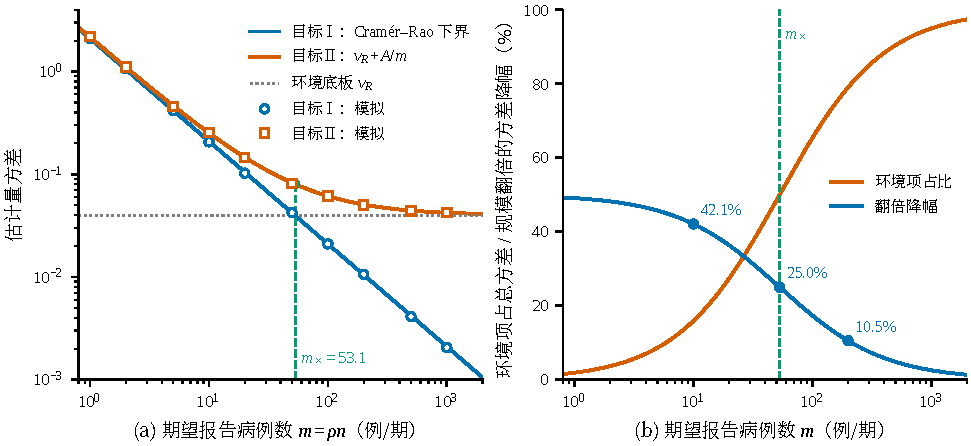
\includegraphics[width=\textwidth]{figures/fig_3_3_variance_theory.pdf}
  \caption{两个估计目标的方差结构。参数为 $\overline{R}=1.15$，$v_R=0.04$，$k=0.35$，$\rho=0.25$，对应 $A=2.1232$，$m_\times=53.1$。（a）目标Ⅰ的方差（取 $R_t=\overline{R}$ 时的 Cramér--Rao 下界）与目标Ⅱ的方差 $v_R+A/m$ 随规模的变化，空心点为每个规模 20,000 次模拟的方差，竖虚线标出交叉点。（b）环境项在目标Ⅱ总方差中的占比与规模翻倍带来的方差降幅，三个标注点对应 $m=10$、$m_\times$ 与 200。}
  \label{fig:variance}
\end{figure}

\subsection{跨环境汇总}
\label{sec:model-pooling}

底板 $v_R$ 在单一环境内无法通过扩大规模消除，但可以通过汇总多个环境来压低。设 $J$ 个辖区的环境方差同为 $v_R$，两两相关系数的平均值为 $\bar c$。等权平均的环境项方差为 $(v_R/J^2)[J+J(J-1)\bar c]$，整理得
\begin{equation}
  v_R\,\bar c+\frac{v_R(1-\bar c)}{J}.
  \label{eq:pooling}
\end{equation}
式~\eqref{eq:pooling} 把底板分成两部分：$v_R\bar c$ 是各辖区共同的环境波动，汇总再多辖区也无法消除；$v_R(1-\bar c)/J$ 是辖区特有的波动，随辖区数增加而下降。各辖区的扰动不完全同步时（$\bar c<1$），汇总能降低底板；完全同步时（$\bar c=1$）汇总无效。这与两阶段抽样中整群内相关决定设计效应的道理相同\citep{kish1965survey}。对流感而言，绝对湿度等气候驱动在相邻地区高度同步\citep{shaman2010absolute}，可以预期 $\bar c$ 不小，汇总能压低的部分有限。第六章用全国加总序列与州级序列的对比估计这一点。

汇总改变的是底板，规模项也会相应变化：汇总后的规模为各辖区规模之和，规模项按总规模缩小。因此跨环境汇总同时作用于两项，交叉点会相应移动，移动方向取决于 $\bar c$ 与辖区数。

\section{报告率与覆盖面}
\label{sec:model-reporting}

\subsection{两条扩容途径的不对称}

$m=\rho n$ 可以通过两条途径扩大，即提高报告率 $\rho$，或扩大覆盖的人群使 $n$ 增大。前者对应提高检测率、改进报告流程，后者对应增加哨点医院、扩大监测辖区。式~\eqref{eq:var-average} 表明两者的作用并不相同。

\begin{proposition}[报告率与覆盖面的不对称]
\label{prop:reporting}
在 H1--H4 下：
\begin{enumerate}[label=(\roman*)]
  \item 固定 $n$ 令 $\rho\to1$，$V\to v_R+\Rbar/n+(\Rbar^2+v_R)/(kn)$，极限严格大于 $v_R$；
  \item 固定 $\rho$ 令 $n\to\infty$，$V\to v_R$；
  \item 报告项可以拆为 $\Rbar/(\rho n)=\Rbar/n+(1-\rho)\Rbar/(\rho n)$，第二部分是漏报带来的额外方差；
  \item 把 $n$ 与 $\rho$ 各提高相同的小比例，前者带来的方差下降是后者的 $A/\Rbar=1+\rho(\Rbar^2+v_R)/(k\Rbar)$ 倍。
\end{enumerate}
\end{proposition}

结论 (i) 与 (ii) 直接由式~\eqref{eq:var-average} 的中间形式得到。$\rho$ 只出现在报告项 $\Rbar/(\rho n)$ 的分母中，超传播项 $(\Rbar^2+v_R)/(kn)$ 不含 $\rho$，所以即使报告完全，超传播项仍然存在。$n$ 同时出现在两项的分母中，扩大覆盖可以把两项都压到零。结论 (iii) 把报告项拆成完整报告时也会存在的部分 $\Rbar/n$ 与漏报带来的额外部分，$\rho=1$ 时后者为零。

结论 (iv) 比较边际效果。对 $\log n$ 求导，两项都按 $1/n$ 变化，方差的变化为 $-A/m$；对 $\log\rho$ 求导，只有报告项变化，方差的变化为 $-\Rbar/m$。两者之比为 $A/\Rbar$。它大于 1，表明在同样的相对增幅下扩大覆盖总是更有效；超出 1 的部分 $\rho(\Rbar^2+v_R)/(k\Rbar)$ 随报告率线性增长，报告率越高、超传播越明显，两条途径的差距越大。

\subsection{不对称的数量大小}

命题~\ref{prop:reporting} 在定性上说明扩大覆盖优于提高报告率，但差距大小取决于 $\rho$。图~\ref{fig:levers} 画出 $A/\Rbar$ 随报告率的变化，横轴为对数刻度，三条曲线对应 $k=0.1$、0.35 和 1，其余参数取示例值。三条曲线都从左侧接近 1 的位置出发，随 $\rho$ 增大而上升，$k$ 越小上升越快。报告完全时（$\rho=1$），三者分别为 12.85、4.39 和 2.18，即在超传播很强的情形下扩大覆盖的边际效果是提高报告率的十余倍。示例参数（$\rho=0.25$，$k=0.35$）对应图中的菱形，$A/\Rbar=1.85$，扩大覆盖的效果接近提高报告率的两倍。$k=0.35$ 时这一比值在 $\rho=0.295$ 处达到 2。

\begin{figure}[!tbp]
  \centering
  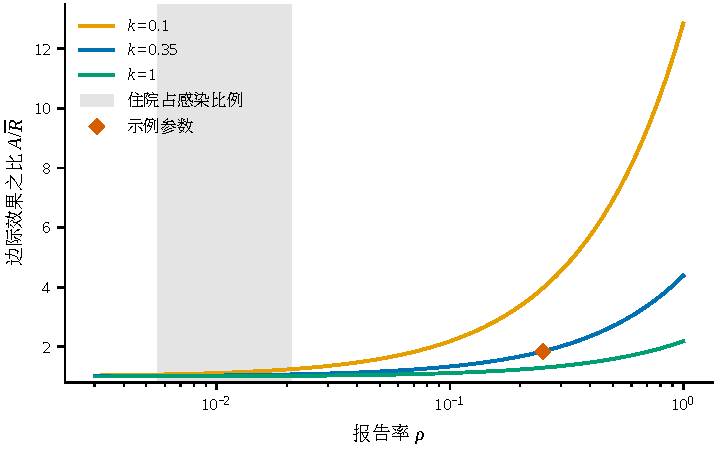
\includegraphics[width=0.72\textwidth]{figures/fig_3_4_levers.pdf}
  \caption{扩大覆盖与提高报告率的边际效果之比 $A/\overline{R}$ 随报告率的变化。$\overline{R}=1.15$，$v_R=0.04$；灰色带为流感住院占感染比例的范围 0.0056--0.021，菱形为示例参数 $\rho=0.25$、$k=0.35$。}
  \label{fig:levers}
\end{figure}

图中灰色带标出流感住院占感染比例的范围，约为 0.0056--0.021\citep{zhou2012hospitalizations, tokars2018seasonal}。在这一范围内三条曲线都贴近 1：$k=0.35$ 时比值为 1.019--1.071。第五章使用的情景参数取 $\Rbar=1.67$、$k\in[0.2,0.5]$，此时这一比值为 1.02--1.18。对住院数据而言，两条途径的边际效果几乎相同，选择哪一条主要看成本。报告率很低时，报告项 $\Rbar/(\rho n)$ 远大于超传播项，方差几乎全部来自报告抽样，提高 $\rho$ 与扩大 $n$ 都在压低同一项。

这一数量判断修正了一个容易产生的误解，即认为超传播使提高报告率在任何情况下都事倍功半。不对称在报告率高、超传播强的情形下才显著，例如接触追踪或暴发调查；在住院、死亡这类报告率很低的监测指标上，两条途径近乎等价。

\section{本章小结}
\label{sec:model-summary}

本章在负二项传播与二项报告的两层模型下，区分了两个估计目标。命题~\ref{prop:current} 表明，对当期再生数，报告病例数除以预计报告规模的估计量在每个有限规模上精确达到 Cramér--Rao 下界，规模收益持续存在，超传播只是让信息打了折扣。命题~\ref{prop:average} 表明，对跨期平均水平，估计方差为环境底板加规模反比项，交叉点 $\mx=A/v_R$ 是两项相等时的规模。规模达到交叉点时再翻一倍只能把方差降低 25\%；曲线处处凸，交叉点是刻度而非阈值。汇总多个环境可以压低底板中辖区特有的部分，共同的环境波动无法通过汇总消除。命题~\ref{prop:reporting} 表明扩大覆盖的边际效果总是不低于提高报告率，两者之比为 $A/\Rbar$，但在住院监测的低报告率下这一比值接近 1。

这些结论依赖 H1--H4，其中 H4 在真实序列中不自动成立。第四章先在 H1--H4 下把方差结构转化为监测设计的定量结论，再用更新过程的模拟考察放宽 H4 后单代公式的适用程度。

\chapter{监测设计含义与数值模拟}
\label{chap:design}

第三章得到的方差结构可以回答三个监测设计问题：总报告量固定时期数与单期规模如何取舍；考虑每期固定成本后单期规模应取多大；规模较小时如何可靠地判断疫情是否在增长。前两个问题属于目标Ⅱ，第三个问题属于目标Ⅰ，两类问题对规模的需求相差一个数量级。第~\ref{sec:design-budget}~节至第~\ref{sec:design-test}~节在 H1--H4 下依次讨论这三个问题。第~\ref{sec:design-renewal}~节放宽 H4，用带环境波动的更新过程考察单代结论在时间序列中的适用程度，为第五章的实证设定提供依据。

\section{多期预算分配}
\label{sec:design-budget}

\subsection{期数与单期规模的取舍}

设共观测 $T$ 期，每期预计报告 $m$ 例，总量 $B=Tm$ 固定。用各期估计的平均值 $T^{-1}\sum_t\widehat R_t$ 估计 $\Rbar$。这对应一个常见的监测选择：在一个流行季内，是少数几次大规模调查，还是多次小规模调查。

\begin{proposition}[多期分配]
\label{prop:allocation}
在 H1--H4 下，若各期 $R_t$ 相互独立，则
\begin{equation}
  \frac{1}{T^2}\Var\Bigl(\sum_{t=1}^{T}\widehat R_t\Bigr)=\frac{v_R}{T}+\frac{A}{B}.
  \label{eq:alloc-indep}
\end{equation}
若 $R_t$ 服从系数为 $r\in(0,1)$ 的平稳一阶自回归过程，规模项仍为 $A/B$，环境项变为
\begin{equation}
  \frac{v_R}{T}\cdot\frac{1+r}{1-r}-\frac{2r(1-r^T)\,v_R}{T^2(1-r)^2}.
  \label{eq:alloc-ar}
\end{equation}
两种情形下，方差都随 $T$ 严格递减。
\end{proposition}

推导仍从全方差公式出发，条件变量取全部 $T$ 期的环境 $(R_1,\dots,R_T)$。给定环境，各期的测量误差由各自的传播与报告产生，由 H1 相互独立，条件方差之和为 $\sum_t[R_t/(\rho n)+R_t^2/(kn)]$，取期望后得到 $TA/m$，除以 $T^2$ 即为 $A/(Tm)=A/B$。这一项只依赖总量 $B$，与如何切分无关，也与环境之间是否相关无关，因为环境的相关性只影响各期 $R_t$ 的联合分布，平稳性保证每期的 $\E R_t$ 与 $\E R_t^2$ 不变。条件均值之和为 $\sum_tR_t$，它的方差就是环境项。各期独立时为 $Tv_R$；一阶自回归时滞后 $h$ 的协方差为 $v_Rr^h$，有
\begin{equation}
  \Var\Bigl(\sum_{t=1}^{T}R_t\Bigr)=v_R\Bigl[T+2\sum_{h=1}^{T-1}(T-h)r^h\Bigr],
  \label{eq:ar-sum}
\end{equation}
对几何级数求和即得式~\eqref{eq:alloc-ar}，这是平稳一阶自回归过程部分和方差的精确表达式\citep{hamilton1994time}。

命题~\ref{prop:allocation} 的直觉很简单。总量固定时，规模项 $A/B$ 是固定成本，切成多少期都一样；环境项则取决于看到了多少个独立的环境实现，期数越多，环境偏离被平均得越充分。只看方差，期数越多越好，极端情形是每期只观测极少的病例。现实中期数不能无限增加，第~\ref{sec:design-optimal}~节引入每期固定成本来处理这一点。

\subsection{有效期数近似的偏差}

时间序列分析中常用有效期数 $T_{\mathrm{eff}}=T(1-r)/(1+r)$ 把相关序列折算为独立序列，环境项近似为 $v_R/T_{\mathrm{eff}}$。这一近似只保留了式~\eqref{eq:alloc-ar} 的第一项，第二项为负，所以近似总会高估环境项。高估的相对大小为第二项与精确值之比，第二项与第一项之比为 $2r(1-r^T)/[T(1-r^2)]$，因此近似只在 $T\gg2r/(1-r^2)$ 时可用。$r=0.8$ 时这一门槛约为 4.4，$r=0.5$ 时约为 1.3。

图~\ref{fig:budget}b 画出高估百分比随期数的变化。两条曲线都随 $T$ 单调下降，$r=0.8$ 的曲线始终在 $r=0.5$ 之上，期数很少时高估成倍。$r=0.8$ 时，$T=26$ 高估 20.5\%，$T=10$ 高估 65.8\%，$T=52$ 仍有 9.35\%；$r=0.5$ 时，三者分别为 5.41\%、15.37\% 和 2.63\%。按周观测的流感季通常只有二三十周，周际环境相关又较强，有效期数近似在这一范围内会明显高估环境项，进而低估增加期数的收益。设计计算应直接使用式~\eqref{eq:alloc-ar}。

\subsection{整数约束}

实际切分还受整数约束。每期需要 $n=B/(\rho T)$ 名感染者，因此 $T$ 必须整除 $B/\rho$。例如 $B=30$、$\rho=0.25$ 时，$B/\rho=120$，可行的 $T$ 为 120 的 16 个因数；$\rho=0.7$ 时 $B/\rho$ 非整数，可行集为空，只能放宽总量。整数约束在理论上无关紧要，在报告率较高、总量较小的设计中会直接决定方案是否可行。

\section{成本最优单期规模}
\label{sec:design-optimal}

\subsection{含固定成本的费用模型}

期数不能无限增加，因为每多观测一期都有固定成本，例如启动一轮调查、召集一次会商或维持一个报告周期。设每期固定成本为 $c_0$，每例预计报告病例的边际成本为 $c_1$，总经费为 $\mathcal B$，于是期数 $T=\mathcal B/(c_0+c_1m)$。

\begin{corollary}[成本最优单期规模]
\label{cor:optimal}
在命题~\ref{prop:allocation} 的独立情形下，估计方差为 $f(m)=(c_0+c_1m)(v_R+A/m)/\mathcal B$。当 $c_0>0$ 时，它在下式处取最小值
\begin{equation}
  m^*=\sqrt{\frac{c_0}{c_1}\,\mx},\qquad
  f(m^*)=\frac{(\sqrt{c_0v_R}+\sqrt{c_1A})^2}{\mathcal B}.
  \label{eq:optimal-m}
\end{equation}
若 $\mathcal B<c_0+c_1m^*$，约束 $T\geq1$ 起作用，最优解取 $T=1$；若 $c_0=0$，最优解为 $m\to0$。
\end{corollary}

把 $T=\mathcal B/(c_0+c_1m)$ 代入 $V(m)/T$ 即得 $f(m)$。展开得
\begin{equation}
  \mathcal B\,f(m)=c_0v_R+c_1A+c_1v_R\,m+\frac{c_0A}{m},
  \label{eq:f-expand}
\end{equation}
前两项为常数，后两项一个随 $m$ 线性增加，一个与 $m$ 成反比。令导数 $c_1v_R-c_0A/m^2$ 为零，得 $m^*=\sqrt{c_0A/(c_1v_R)}=\sqrt{(c_0/c_1)\mx}$；二阶导数 $2c_0A/m^3>0$，驻点为最小值。代回后两项相等，均为 $\sqrt{c_0c_1v_RA}$，合并即得 $f(m^*)$。若 $c_0=0$，后一项消失，$f$ 随 $m$ 单调增加，回到命题~\ref{prop:allocation} 的结论，即没有固定成本时，期数越多越好。

式~\eqref{eq:f-expand} 揭示了权衡的两端。$c_1v_Rm$ 对应单期规模过大，经费集中在少数几期，看到的环境实现太少；$c_0A/m$ 对应单期规模过小，期数太多，固定成本挤占了病例经费，每期的测量误差偏大。最优单期规模是成本比 $c_0/c_1$ 与交叉点 $\mx$ 的几何平均。固定成本相对越高，每期越应多收集病例；交叉点越大，即环境越稳定或测量噪声越大，每期也越应多收集病例。最优规模与总经费 $\mathcal B$ 无关，经费增加只改变期数。

\subsection{与两阶段抽样的同构}

推论~\ref{cor:optimal} 与两阶段抽样的费用最优分配是同一个问题\citep{cochran1977sampling}。对照式~\eqref{eq:two-stage} 与式~\eqref{eq:cochran-opt}，期数 $T$ 对应初级单元数，$v_R$ 对应初级单元间方差 $S_b^2$，$A$ 对应单元内方差 $S_w^2$，$c_0$ 与 $c_1$ 分别对应初级单元与次级单元的单位成本 $c_1'$、$c_2'$。两个最优解的形式完全相同，都是费用比与方差比之积的平方根。

同构也提示了差别所在。两阶段抽样中初级单元按设计独立抽取，监测中的各期环境存在时间相关；抽样中单元内样本量由设计者决定，监测中的规模由此前的传播产生。前一个差别在下文的自相关修正中处理，后一个差别对应 H4，在第~\ref{sec:design-renewal}~节讨论。

\subsection{数值示例}

按第五章的情景参数，交叉点 $\mx$ 在 21.3--49.2。$c_0/c_1=10$ 时 $m^*$ 为 14.6--22.2，$c_0/c_1=100$ 时为 46.1--70.1。在第三章的示例参数下（$\mx=53.1$），两种成本比对应的 $m^*$ 分别为 23.0 和 72.9。成本比扩大 10 倍，最优规模只扩大约 3.2 倍，这是平方根关系的直接结果。

连续解需要取整后才能执行。取示例参数，$c_0=100$，$c_1=1$，$\mathcal B=600$，连续解为 $m^*=72.86$，对应方差 $f(m^*)=0.01992$，此时 $T=600/172.86$ 不是整数。表~\ref{tab:integer-alloc} 逐个列出整数 $T$ 下的方案，单期规模由 $m=\mathcal B/T-c_0$ 得到。

\begin{table}[!tbp]
  \centering
  \caption{固定经费下整数期数方案的比较}
  \label{tab:integer-alloc}
  \begin{tabular}{@{}cccc@{}}
    \toprule
    期数 $T$ & 单期规模 $m$ & 估计方差 & 与连续最优之比 \\
    \midrule
    1 & 500 & 0.04425 & 2.22 \\
    2 & 200 & 0.02531 & 1.27 \\
    3 & 100 & 0.02041 & 1.02 \\
    4 & 50 & 0.02062 & 1.04 \\
    5 & 20 & 0.02923 & 1.47 \\
    \bottomrule
  \end{tabular}

  \vspace{4pt}
  {\small 注：$\overline{R}=1.15$，$v_R=0.04$，$k=0.35$，$\rho=0.25$，$c_0=100$，$c_1=1$，$\mathcal{B}=600$；连续最优为 $m^*=72.86$，方差 0.01992。}
\end{table}

最优整数方案是 $T=3$、$m=100$，方差 0.02041，只比连续最优高约 2.5\%；$T=4$、$m=50$ 次之。把经费全部投入一期（$T=1$）的方差是最优方案的两倍多，切成五期（$T=5$）则因固定成本占去大部分经费，每期只剩 20 例，方差也明显偏高。图~\ref{fig:budget}a 画出连续目标函数与五个整数方案。曲线在 $m^*$ 左侧陡峭、右侧平缓：规模不足时方差上升很快，规模偏大时上升较慢。这一不对称来自式~\eqref{eq:f-expand} 中反比项与线性项的形状差异，它意味着在参数不确定时，宁可把单期规模取得略大一些。

\begin{figure}[!tbp]
  \centering
  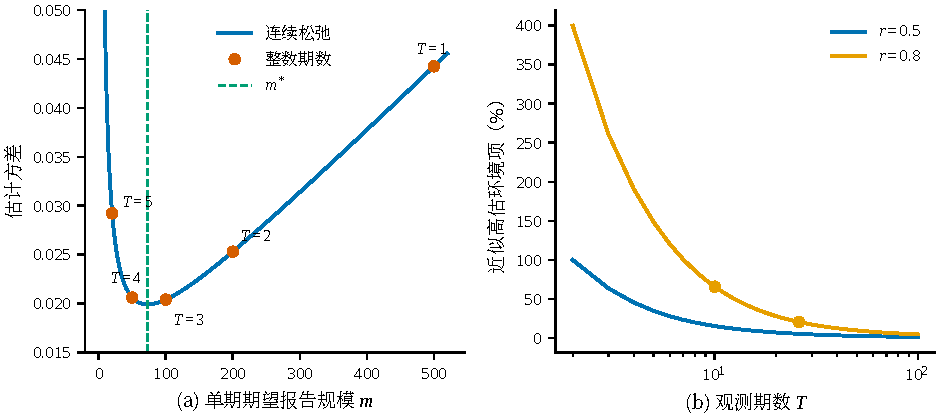
\includegraphics[width=\textwidth]{figures/fig_4_1_budget.pdf}
  \caption{预算分配的两个侧面。（a）固定经费下估计方差随单期规模的变化，$c_0=100$，$c_1=1$，$\mathcal{B}=600$，其余参数取示例值；曲线为连续松弛，圆点为整数期数方案，竖虚线为连续最优 $m^*$。（b）环境服从一阶自回归时，有效期数近似相对精确式高估环境项的百分比随观测期数的变化，圆点标出 $r=0.8$ 时 $T=10$ 与 $T=26$。}
  \label{fig:budget}
\end{figure}

\subsection{自相关修正}

若环境服从一阶自回归，式~\eqref{eq:alloc-ar} 的第一项相当于把环境方差放大为 $v_R(1+r)/(1-r)$，交叉点相应缩小为原来的 $(1-r)/(1+r)$ 倍，$m^*$ 应乘以约 $\sqrt{(1-r)/(1+r)}$。最优方案因而偏向更多、更小的期。这一方向初看有违直觉：相邻各期的环境相似，多观测一期带来的新信息变少，似乎应当减少期数。决定权衡的却是两项的相对大小。环境项被放大后，规模项在总方差中的份额下降，压低环境项的边际价值相对上升，而压低环境项只能靠增加期数。

仍取示例参数与 $c_0/c_1=100$，$r=0.5$ 时数值求得的精确最优与近似值分别为 42.9 和 42.1，$r=0.8$ 时分别为 25.0 和 24.3。近似值比精确值略小，这与有效期数近似高估环境项的方向一致，二者相差不到 1 例，近似在设计中够用。

\section{精确增长检验}
\label{sec:design-test}

\subsection{检验的构造}

监测中最常见的判断是疫情是否在增长，即检验 $H_0\colon R_t\leq1$ 对 $H_1\colon R_t>1$。这是目标Ⅰ层面的问题，误差只来自测量，规模的作用持续存在。

\begin{proposition}[精确增长检验]
\label{prop:test}
在 H1--H3 下，$C_t$ 的分布族关于 $R_t$ 具有单调似然比。令 $c_\alpha$ 为满足 $P_{R_t=1}(C_t\geq c)\leq\alpha$ 的最小整数，检验在 $C_t\geq c_\alpha$ 时拒绝 $H_0$。该检验有以下三条性质。
\begin{enumerate}[label=(\roman*)]
  \item 第一类错误概率在 $R_t\leq1$ 上的上确界在 $R_t=1$ 处取得，实际水平 $\alpha^*\leq\alpha$。
  \item 该检验在水平 $\alpha^*$ 下一致最优；加入随机化的 Karlin--Rubin 检验恰好达到水平 $\alpha$，并在该水平下一致最优。
  \item 在 $R_t=1+\delta$ 处的功效为
  \begin{equation}
    \pi(n,\delta)=1-F_{\NB}\bigl(c_\alpha-1;\ nk,\ k/[k+\rho(1+\delta)]\bigr).
    \label{eq:power}
  \end{equation}
\end{enumerate}
\end{proposition}

单调似然比性质可以直接验证。取 $R_2>R_1$，由式~\eqref{eq:report-dist}，似然比为
\begin{equation}
  \frac{f(c;R_2)}{f(c;R_1)}=\Bigl(\frac{k+\rho R_1}{k+\rho R_2}\Bigr)^{nk}
  \Bigl[\frac{R_2(k+\rho R_1)}{R_1(k+\rho R_2)}\Bigr]^{c},
  \label{eq:mlr}
\end{equation}
方括号内的底数大于 1，因为 $R_2k+\rho R_1R_2>R_1k+\rho R_1R_2$，所以似然比随 $c$ 递增。由 Karlin--Rubin 定理，形如 $\{C_t\ge c\}$ 的拒绝域在它自身的实际水平下一致最优，拒绝概率随 $R_t$ 递增，零假设下的最大第一类错误概率出现在边界 $R_t=1$ 处\citep{karlin1956theory, lehmann2005testing}。功效公式~\eqref{eq:power} 是负二项分布函数在临界值处的直接计算。

这里的“一致最优”需要限定。非随机化检验只能在 $\alpha^*$ 这个离散的水平上一致最优；要在名义水平 $\alpha$ 上最优，需要在 $C_t=c_\alpha-1$ 时以一定概率随机拒绝，这在监测实践中难以接受。命题~\ref{prop:test} 还依赖 $k$ 已知；若 $k$ 用数据估计，水平不再有精确保证。$k$ 设得过大会低估方差，临界值偏低，实际水平随之偏高；设得过小则检验偏保守。

\subsection{Wald 检验的水平失真}

实际工作中常用正态近似的 Wald 检验，即把 $(\widehat R_t-1)/\sqrt{V_0}$ 与正态分位数比较，其中 $V_0=1/(\rho n)+1/(kn)$ 是 $R_t=1$ 时的方差。该检验的实际水平同样可以用负二项分布函数精确算出，不需要模拟。

图~\ref{fig:test}a 给出名义水平为 5\% 时两种检验的实际水平。彩色点为 Wald 检验，三种颜色对应三个 $k$ 值；灰色点为精确检验。Wald 检验在小规模时系统性地超过名义水平，点群整体落在 5\% 虚线之上，并随规模增大逐渐向虚线靠拢。$k=0.1$、$m=5$ 时实际水平为 7.81\%；在 $m<40$ 的范围内，$k=0.1$、0.35 和 1 的最大实际水平分别为 8.03\%、8.75\% 和 10.40\%。精确检验的点全部在虚线以下，整个网格上的最大水平为 0.05000，没有超出名义水平。两种检验的点都呈锯齿状排列，这是离散分布下临界值逐格跳动的结果。

Wald 检验偏离的原因是负二项分布在小规模时右偏明显。右偏分布的上尾比正态分布厚，用正态分位数作临界值会把过多的零假设样本判为增长。这与 Brown 等在二项比例区间中发现的问题同类\citep{brown2001interval}，负二项计数的偏度还要更大。对监测实践而言，若用 Wald 检验在小辖区每周判断增长，误报的频率会比预设高出一半到一倍。

\begin{figure}[!tbp]
  \centering
  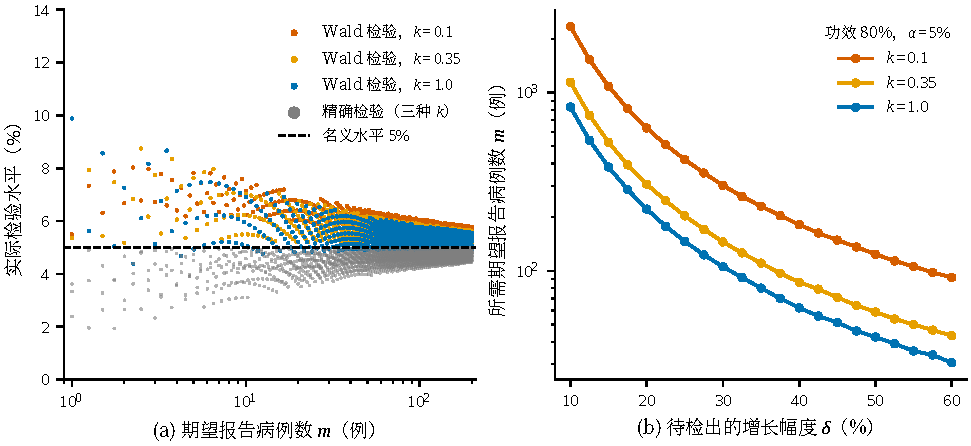
\includegraphics[width=\textwidth]{figures/fig_4_3_growth_test.pdf}
  \caption{增长检验的实际水平与所需规模，$\rho=0.25$，名义水平 5\%，全部由负二项分布函数精确计算。（a）Wald 检验（按 $k$ 着色）与精确检验（灰色）的实际水平随期望报告规模的变化；（b）达到并保持 80\% 功效所需的期望报告规模与待检出增长幅度 $\delta$ 的关系。}
  \label{fig:test}
\end{figure}

\subsection{功效的锯齿与所需规模}

功效随 $n$ 的变化不是单调的。$c_\alpha$ 只能取整数，每当它跳升一格，实际水平骤降，功效也随之短暂下降。以 $k=0.35$、$\delta=0.3$ 为例，$n$ 从 400 增加到 699 的过程中，功效下降了 82 次。因此只报告“首次达到 80\% 功效的规模”并不够，略大一点的规模可能又跌回 80\% 以下；更稳妥的指标是“此后始终保持 80\% 以上的最小规模”。表~\ref{tab:power-n} 同时列出两者。

\begin{table}[!tbp]
  \centering
  \caption{增长检验达到 80\% 功效所需的感染者人数}
  \label{tab:power-n}
  \begin{tabular}{@{}cccc@{}}
    \toprule
    离散参数 $k$ & 增长幅度 $\delta$ & 首次达到 & 此后保持 \\
    \midrule
    0.35 & 0.15 & 2071 & 2107 \\
    0.35 & 0.30 & 568 & 581 \\
    0.35 & 0.50 & 229 & 235 \\
    1 & 0.25 & 568 & 585 \\
    0.1 & 0.25 & 1660 & 1684 \\
    \bottomrule
  \end{tabular}

  \vspace{4pt}
  {\small 注：$\rho=0.25$，名义水平 5\%，单侧检验；表中为上一代感染者人数 $n$，预计报告规模为 $m=\rho n$。}
\end{table}

表~\ref{tab:power-n} 有三点规律。增长幅度越小，所需规模越大，$\delta$ 从 0.5 降到 0.15，所需人数扩大约 9 倍，大致与 $\delta^{-2}$ 成比例，这是正态近似下功效计算的一般规律。离散参数越小，所需规模越大，$\delta=0.25$ 时 $k=0.1$ 所需人数约为 $k=1$ 的 2.9 倍，超传播让每一个病例携带的信息变少。首次达到与此后保持之间的差距为 6 至 36 人，相对差距在 1\% 至 3\% 之间，绝对值不大，但在规模本已较大时，按首次达到的数字设计会有一段规模区间功效不足。图~\ref{fig:test}b 以预计报告规模为纵轴画出保持 80\% 功效所需的规模，三条曲线随 $\delta$ 增大而下降，$k$ 越小曲线越高，规律与表~\ref{tab:power-n} 一致。

这些数字与第三章的交叉点形成对照。$k=0.35$ 时，要稳定检出 15\% 的增长，每期需要约 2107 名感染者，即 $m\approx527$ 例预计报告，是示例交叉点的十倍左右。对目标Ⅱ而言，规模过了 $\mx$ 收益就明显变小；对判断当期增长这类目标Ⅰ问题，规模的价值要大得多。同一套监测数据服务于不同目标时，规模是否“够用”的答案可以完全不同。

\section{时间序列中的规模效应}
\label{sec:design-renewal}

\subsection{随机分母问题}

前几节假定上一代感染者人数 $n$ 已知。真实监测序列不满足这一点。下一周的新感染由此前几周的感染共同产生，感染压力可写为 $\Lambda_{t+1}=\sum_{s\geq1}w_sI_{t+1-s}$，其中 $w_s$ 是世代间隔分布。漏报使 $I_1,\dots,I_t$ 无法完全观测，所以下一周的感染压力 $\Lambda_{t+1}$ 也是随机的。实际能用的只是报告数的加权和
\begin{equation}
  D_t=\sum_{s\geq1}w_sC_{t+1-s},
  \label{eq:dt}
\end{equation}
并以 $G_t=C_{t+1}/D_t$ 作为增长统计量。$D_t$ 在这里扮演了 $m=\rho n$ 的角色，但它本身含有报告噪声，是一个随机分母。

预测误差取决于可用的信息集。记 $\mathcal F_t$ 为截至第 $t$ 周的全部报告，$m=\rho\,\E(\Lambda_{t+1}\mid\mathcal F_t)$。

\begin{remark}
\label{rem:information}
设给定 $\Lambda_{t+1}$ 与 $R_{t+1}$ 时，$C_{t+1}$ 服从式~\eqref{eq:report-dist} 中以 $\Lambda_{t+1}$ 代替 $n$ 的负二项分布，且在 $\mathcal F_t$ 条件下 $\Lambda_{t+1}$ 与 $R_{t+1}$ 独立。两次使用全方差公式，可得
\begin{equation}
  \frac{\Var(C_{t+1}\mid\mathcal F_t)}{[\rho\,\E(\Lambda_{t+1}\mid\mathcal F_t)]^2}
  =v_R+\frac{A}{m}+\CV^2(\Lambda_{t+1}\mid\mathcal F_t)\,(\Rbar^2+v_R).
  \label{eq:info-decomp}
\end{equation}
当 $\Lambda_{t+1}$ 完全已知时，变异系数项为零，式~\eqref{eq:info-decomp} 退化为命题~\ref{prop:average}。
\end{remark}

注~\ref{rem:information} 的推导分两层。第一层条件于 $(\Lambda_{t+1},R_{t+1})$，条件均值为 $\rho\Lambda_{t+1}R_{t+1}$，条件方差的期望按命题~\ref{prop:average} 的方式处理，得到规模项。第二层计算条件均值 $\rho\Lambda_{t+1}R_{t+1}$ 在 $\mathcal F_t$ 下的方差，利用 $\Lambda_{t+1}$ 与 $R_{t+1}$ 条件独立，乘积的方差拆为 $\E(\Lambda^2)\E(R^2)-[\E\Lambda\,\E R]^2$，除以 $(\rho\E\Lambda)^2$ 后得到 $v_R$ 与 $\CV^2(\Lambda)(\Rbar^2+v_R)$ 两项。多出的一项来自感染压力的不确定性，它与规模无关。漏报使感染压力无法由报告精确还原，因此这一项在实际序列中一般不为零。

\subsection{误差指标的两种读法}

第五章使用的误差指标有两种读法。用 $\Rbar D_t$ 预测 $C_{t+1}$ 的相对误差，与用 $G_t$ 估计 $\Rbar$ 的相对误差恒等：
\begin{equation}
  \frac{(C_{t+1}-\Rbar D_t)^2}{(\Rbar D_t)^2}=\frac{(G_t-\Rbar)^2}{\Rbar^2}.
  \label{eq:identity}
\end{equation}
左端是预测问题，右端是估计问题，二者在数值上相同。这使第五、六章可以用预测误差检验估计误差的形状。记 $\mu_t=\E(C_{t+1}\mid\mathcal F_t)$，$\sigma_t^2=\Var(C_{t+1}\mid\mathcal F_t)$。由于 $D_t$ 由 $\mathcal F_t$ 决定，增长统计量的均方误差可以分解为
\begin{equation}
  \E[(G_t-\Rbar)^2]=\E[(\sigma_t/D_t)^2]+\E[(\mu_t/D_t-\Rbar)^2].
  \label{eq:mse-decomp}
\end{equation}
第二项是条件偏差，非负。第一项则不必等于 $v_R+A/D_t$，因为 $D_t$ 只是 $\rho\Lambda_{t+1}$ 的带噪代理，$(\sigma_t/D_t)^2$ 可能高于也可能低于单代公式。因此，单代公式 $(v_R+A/m)/\Rbar^2$ 在时间序列中只能作参照曲线，一般情况下不构成下界。

\subsection{仿真设计}

为了解参照曲线的偏离程度，模拟一个带环境波动的更新过程。世代间隔取 4 周离散核，权重依次为 0.45、0.35、0.15、0.05，与第二章所述流感序列间隔短于一周的证据\citep{cowling2009estimation, vink2014serial}相符，大部分传播发生在一至两周内。每周 $R_t$ 独立抽自均值 1.15、方差 0.04 的 Gamma 分布；$I_t\sim\NB(k\Lambda_t,\,k/(k+R_t))$，$k=0.35$；报告数 $C_t\sim\Bin(I_t,0.25)$。参数与第三章示例一致，单代参照曲线因而可以直接用 $A=2.1232$ 计算。

为避免轨迹灭绝，$I_t$ 截断为不小于 1。前 4 周的感染数设为 $m_0/\rho$，使初始每周期望报告 $m_0$ 例，$m_0$ 取 6 到 800 共 8 档。每档模拟 400 条 30 周的轨迹，前 4 周为初始化，每条有 26 个评价点，随机种子为 20261014。截断只在小规模时发生，$m_0=6$ 与 12 时的比例分别为 1.42\% 与 0.16\%，$m_0\geq25$ 时为零，因此截断对 $m_0\ge25$ 的结果没有影响。

\subsection{仿真结果}

图~\ref{fig:renewal} 给出结果。左图纵轴为增长统计量的相对均方误差，横轴为初始规模 $m_0$，实线为单代参照曲线，点线为环境底板 $v_R/\Rbar^2$。模拟误差总体沿参照曲线下降并趋于底板，“常数加规模反比”的形状清晰可见；但在 $m_0$ 较大的几档，模拟点落在参照曲线下方，在最小的两档则高出参照曲线很多。

\begin{figure}[!tbp]
  \centering
  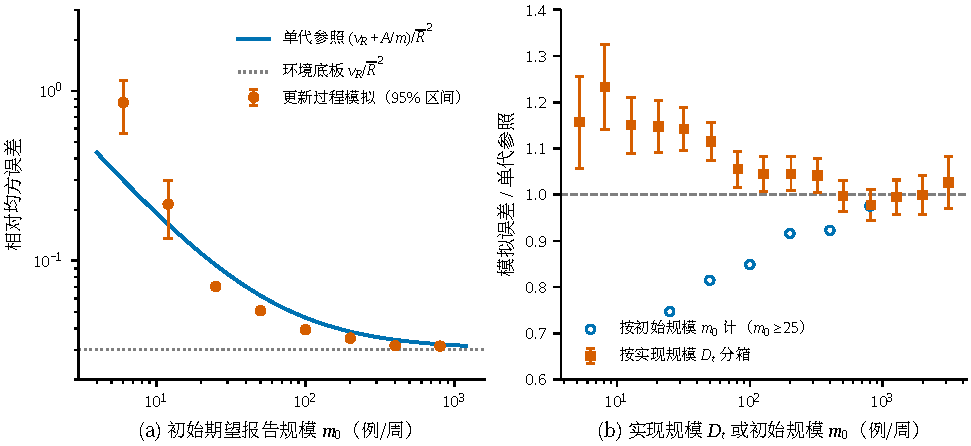
\includegraphics[width=\textwidth]{figures/fig_4_4_renewal_scale.pdf}
  \caption{更新过程仿真中的规模效应。每个初始规模 400 条轨迹，每条 26 个评价点，误差棒为 95\% 区间。（a）增长统计量的相对均方误差随初始规模 $m_0$ 的变化，实线为单代参照曲线 $(v_R+A/m)/\overline{R}^2$，点线为环境底板，参照曲线不是误差下界。（b）模拟误差与参照曲线之比，方块按实际规模 $D_t$ 分组，空心圆按初始规模 $m_0$（$m_0\geq25$）计算。}
  \label{fig:renewal}
\end{figure}

右图把误差与参照曲线之比按两种规模口径分别画出，两种口径给出相反的结论。按初始规模 $m_0$ 计，$m_0\geq25$ 时模拟误差是参照曲线的 0.75--0.98 倍，低于参照。原因是 $\Rbar>1$，疫情在评价期内增长，实际规模高于初始规模，$D_t/m_0$ 的中位数为 1.86--2.35；用初始规模作横轴，等于把较大规模的误差记在了较小规模名下。

按实际规模 $D_t$ 分组，结论反过来。$D_t<400$ 时模拟误差是参照的 1.04--1.23 倍，高于参照，多出的部分来自随机分母：$D_t$ 偶然偏小时，$G_t$ 的分母被低估，比值被放大，而 $1/D_t$ 是凸函数，分母的对称噪声会抬高平均误差。$D_t\geq400$ 时比值为 0.98--1.03，两者基本重合，此时 $D_t$ 中的报告噪声相对很小，随机分母问题消失。

$m_0$ 很小时误差分布有重尾。$m_0=12$ 时比值为 1.31；$m_0=6$ 时为 2.87，且标准误很大，这一数值不稳定。小规模时偶尔出现的近零分母会产生极大的比值，少数几个极端值就能主导均方误差。

由此可以得到两点结论。第一点关于口径：参照曲线是高估还是低估误差，取决于横轴用哪种规模。按实际规模计，“常数加规模反比”的形状大体成立，小规模处误差略高，这为第五章用 $a+b/D_t$ 拟合实证误差提供了依据，也提示第五章的横轴应取实际规模 $D_t$。第二点关于 H4：仿真中各周 $R_t$ 相互独立，$D_t$ 与当期环境无关，H4 在条件意义上仍然成立。真实数据中 $R_t$ 有时间相关，规模大的时期往往也是 $R$ 偏高的时期，H4 不再成立，这会进一步抬高实证截距与斜率。第五章对截距与斜率的分析将回到这一点。

\section{本章小结}
\label{sec:design-summary}

本章把第三章的方差结构转化为三类监测设计结论，并检验了单代结论在时间序列中的适用程度。总报告量固定时，规模项与切分方式无关，期数越多环境项越小。环境存在一阶自回归相关时，常用的有效期数近似会高估环境项，流感季常见的二三十周、强相关情形下高估可达两成到六成以上。引入每期固定成本后，成本最优单期规模是成本比与交叉点的几何平均，与两阶段抽样的费用最优分配同构。整数约束下的最优方案与连续解相差约 2.5\%，正相关使最优方案偏向更多、更小的期。判断当期增长时，Wald 检验在小规模下超出名义水平，基于负二项分布函数的精确检验可以控制水平；稳定检出 15\% 的增长需要约十倍于示例交叉点的规模。

更新过程仿真表明，真实序列中的分母是随机的，单代公式只能作参照曲线。按实际规模计，误差形状与参照曲线大体一致，小规模处偏高；按初始规模计则偏低。第五章将以实际规模为横轴，在美国流感住院数据上检验“常数加规模反比”的误差形状。

\chapter{美国流感住院数据实证}
\label{chap:empirical}

第三章给出的方差结构 $v_R+A/m$ 有一个可以在数据中检验的推论：在环境围绕同一均值波动的时段内，增长统计量的相对误差应当随规模下降，并趋于一个与规模无关的常数。第四章的更新过程仿真进一步说明，在时间序列中检验这一形状时，横轴应取实际规模 $D_t$，单代公式只能作参照曲线。本章用美国国家医疗安全网络的州级流感住院周报检验这一形状。第~\ref{sec:emp-data}~节说明数据、规模测度与填报制度分期。第~\ref{sec:emp-method}~节给出误差指标与估计方法。第~\ref{sec:emp-early}~节报告流行初期的规模效应。第~\ref{sec:emp-inflation}~节分析拟合截距与斜率高于理论值的原因。第~\ref{sec:emp-peak}~节与第~\ref{sec:emp-policy}~节分别考察流行达峰和填报制度变化时误差形状的变化。替代设定、空间汇总与外部数据留在第六章。

\section{数据与变量}
\label{sec:emp-data}

\subsection{数据来源与样本}

数据来自美国国家医疗安全网络（National Healthcare Safety Network，NHSN）公布的各辖区每周实验室确诊流感住院数，以及各辖区填报医院所占的比例\citep{cdc2026nhsn}。样本覆盖 50 个州与华盛顿特区，共 51 个辖区，时间从 2020 年 10 月至 2026 年 9 月，合计 16,218 个州周。其中 504 个州周的住院数缺失，468 个在下文的第一期，36 个在第二期。缺失按 0 处理。这一处理在强制填报期影响很小，在自愿填报期则可能把未填报误记为零住院，第~\ref{sec:emp-policy}~节解读第二期结果时会回到这一点。

选择住院数据首先是因为住院是流感监测中口径最稳定、报告最及时的指标之一，各州按统一定义每周上报，适合作跨辖区比较。此外，住院占感染的比例很低，文献估计在 0.0056--0.021 之间\citep{zhou2012hospitalizations, tokars2018seasonal}。按第三章命题~\ref{prop:reporting} 的数量分析，此时扩大覆盖与提高报告率的边际效果几乎相同，规模项主要由报告抽样决定，模型结构相对简单。

\subsection{规模测度与增长统计量}

第四章式~\eqref{eq:dt} 把规模定义为此前各周报告数按世代间隔加权的和。实证中取三周权重
\begin{equation}
  D_t=0.65\,C_t+0.25\,C_{t-1}+0.10\,C_{t-2},
  \label{eq:dt-main}
\end{equation}
其中 $C_t$ 为第 $t$ 周的住院数。相对于待预测的 $C_{t+1}$，三项的滞后分别为 1、2、3 周，平均回溯滞后为 $0.65\times1+0.25\times2+0.10\times3=1.45$ 周，约 10.2 天。权重集中在最近一周，与流感序列间隔短于一周的证据相符\citep{cowling2009estimation, vink2014serial}；第~\ref{sec:emp-inflation}~节比较另外两种权重。增长统计量取 $G_t=C_{t+1}/D_t$。小规模时 $G_t$ 的分母接近零，比值极不稳定，因此只保留 $D_t\geq5$ 的州周，得到 10,303 个有效观测。

$G_t$ 与第三章的 $R_t$ 不是同一个量。流感的世代间隔约 3 天，一周约跨两代传播，$G_t$ 是两代左右增长的合成，其均值与方差都不等于单代再生数的均值与方差。实证检验因而只使用模型的结构，即相对误差随规模变化的形状；拟合得到的系数描述的是 $G_t$ 这一统计量的误差，不解读为单代参数 $v_R$ 与 $A$ 的估计。这一区分贯穿本章和第六章。

\subsection{填报制度分期}

样本期内 NHSN 的填报制度变过两次。2020 年 10 月至 2024 年 4 月 30 日为强制填报，下称第一期。2024 年 5 月 1 日至 10 月 31 日改为自愿填报，下称第二期。2024 年 11 月 1 日起，美国联邦医疗保险与医疗补助服务中心恢复强制要求，下称第三期。表~\ref{tab:policy} 列出三期的样本量与填报率。第一期与第三期的平均填报率都在 91\% 以上。第二期降到 54.6\%，中位数只有 45.7\%，约一半辖区的填报医院不足半数。

\begin{table}[!tbp]
  \centering
  \caption{三个填报制度期的样本与周增长比的分布特征}
  \label{tab:policy}
  \begin{tabular}{@{}lccc@{}}
    \toprule
    指标 & 第一期（强制） & 第二期（自愿） & 第三期（恢复强制） \\
    \midrule
    有效州周数 & 6,009 & 420 & 3,874 \\
    平均填报率（\%） & 91.1 & 54.6 & 91.8 \\
    填报率中位数（\%） & 92.3 & 45.7 & 93.2 \\
    $G_t$ 均值 & 1.066 & 0.966 & 1.084 \\
    $G_t$ 标准差 & 0.624 & 1.823 & 0.649 \\
    $G_t$ 四分位距 & 0.638 & 0.594 & 0.652 \\
    $G_t$ 中位绝对偏差 & 0.298 & 0.299 & 0.292 \\
    $G_t$ 第 10 百分位数 & 0.468 & 0.199 & 0.508 \\
    $G_t$ 第 90 百分位数 & 1.772 & 1.459 & 1.914 \\
    $G_t$ 偏度 & 3.29 & 14.98 & 2.68 \\
    $G_t$ 最大值 & 12.7 & 33.9 & 11.5 \\
    \bottomrule
  \end{tabular}

  \vspace{4pt}
  {\small 注：有效州周指 $D_t\geq5$ 的州周；三期的有效州周合计 10,303 个。}
\end{table}

图~\ref{fig:nhsn} 画出全国周住院合计与平均填报率。住院数呈明显的季节性，每年 10 月前后开始上升，12 月至次年 2 月达峰，三个流行季的峰高逐季增加。填报率在第二期断崖式下降，第三期恢复后与第一期相当。图中绿色区间是第~\ref{sec:emp-early}~节使用的流行初期窗口，三个窗口都落在强制填报期内，窗口内的数据不受第二期填报率下降的影响。

\begin{figure}[!tbp]
  \centering
  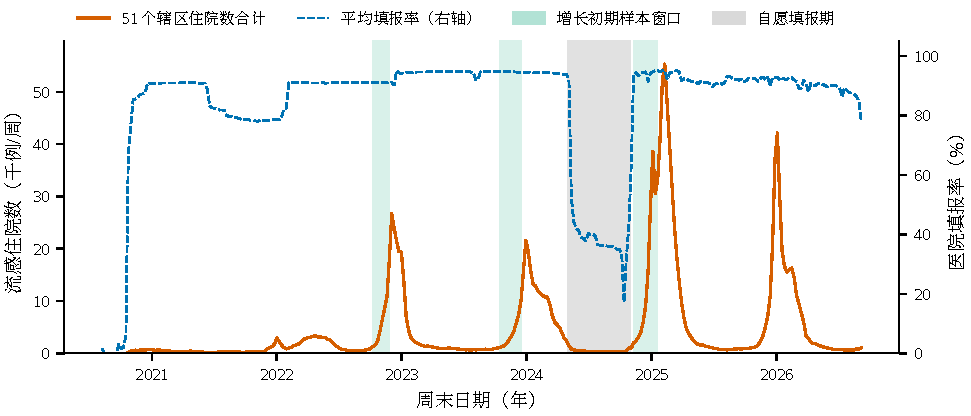
\includegraphics[width=\textwidth]{figures/fig_5_1_nhsn_series.pdf}
  \caption{美国 51 个辖区每周流感住院数合计（实线，左轴）与医院平均填报率（虚线，右轴）。缺失按 0 计入合计；绿色区间为三个流行季的增长初期样本窗口，灰色区间为 2024 年 5--10 月的自愿填报期。}
  \label{fig:nhsn}
\end{figure}

\section{误差指标与估计方法}
\label{sec:emp-method}

\subsection{相对均方误差}

误差指标采用相对均方误差。以某一阶段的平均增长比 $\Rbar$ 为基准，第 $t$ 周的损失定义为
\begin{equation}
  L_t=\Bigl(\frac{G_t-\Rbar}{\Rbar}\Bigr)^2 .
  \label{eq:loss}
\end{equation}
由第四章式~\eqref{eq:identity}，$L_t$ 也是用 $\Rbar D_t$ 预测 $C_{t+1}$ 的相对误差平方，属于预测评价中常用的相对误差评分\citep{bosse2023scoring}。这一恒等关系使下文可以在预测与估计两种读法之间切换。作为预测误差，$L_t$ 衡量以阶段均值外推一周的准确程度。作为估计误差，$L_t$ 衡量单周增长比偏离阶段均值的程度，对应目标Ⅱ。

在单代模型下，以预计报告规模 $m$ 代替 $D_t$，由命题~\ref{prop:average} 两边同除以 $\Rbar^2$，得到损失的条件期望
\begin{equation}
  \E(L_t\mid D_t)\approx a+\frac{b}{D_t},\qquad a=\frac{v_R}{\Rbar^2},\quad b=\frac{A}{\Rbar^2},\quad \frac ba=\mx .
  \label{eq:affine}
\end{equation}
式~\eqref{eq:affine} 是本章的拟合形式。截距 $a$ 对应环境底板，斜率 $b$ 对应规模项，比值 $b/a$ 称为经验交叉点。第四章第~\ref{sec:design-renewal}~节已经说明，在时间序列中 $D_t$ 只是 $\rho\Lambda_{t+1}$ 的带噪代理，式~\eqref{eq:affine} 的第一项与单代公式未必相等，条件偏差项也不为零。因此式~\eqref{eq:affine} 在这里是一个检验形状的工作模型，其系数是否等于 $v_R/\Rbar^2$ 与 $A/\Rbar^2$ 需要单独分析。

\subsection{可行广义最小二乘与聚类重抽}

损失的方差随规模变化。规模小时，$G_t$ 的分母噪声大，损失分布高度右偏；规模大时，损失集中在截距附近。普通最小二乘对所有观测等权，小规模观测的大方差会主导拟合。为此采用可行广义最小二乘\citep{wooldridge2010econometric}：第一步用普通最小二乘得到拟合值 $\hat\mu_t=\hat a+\hat b/D_t$；第二步以 $1/\hat\mu_t^2$ 为权重重新拟合。若损失近似服从变异系数恒定的分布，其方差与均值的平方成正比，$1/\hat\mu_t^2$ 即为近似最优权重。

区间估计采用按州聚类的自助法\citep{cameron2008bootstrap, cameron2015practitioner}。同一州相邻各周的损失相关，按州整体重抽可以保留州内的时间相关结构。重抽 1,500 次，每次重复两步估计，取 2.5\% 与 97.5\% 分位数作为 95\% 区间。经验交叉点的区间由每次重抽的 $\hat b/\hat a$ 直接取分位数，不依赖比值的正态近似。分箱均值的区间同样由按州聚类的重抽给出。

\section{流行初期的规模效应}
\label{sec:emp-early}

\subsection{样本窗口}

模型假定各期环境围绕同一均值波动。流行初期病例持续增长，传播水平相对稳定，最接近这一情形，所以主分析取三个流行季的增长初期，即 2022 年 10 月 8 日至 11 月 26 日、2023 年 10 月 14 日至 12 月 16 日、2024 年 11 月 9 日至 2025 年 1 月 18 日。窗口内共 1,267 个有效州周，平均增长比 $\Rbar_{\mathrm{early}}=1.6706$，标准差 0.7116。平均增长比大于 1，说明窗口内住院数平均每周增长约三分之二。2020--2021 和 2021--2022 两季受 2019 冠状病毒病大流行期间防控措施的影响，流感活动低且不规则，没有纳入初期窗口。

\subsection{分箱结果}

表~\ref{tab:early-bins} 按 $D_t$ 把初期样本分为六箱。平均损失从最小箱的 0.329 降到 $[20,50)$ 箱的 0.160，再降到 $[100,250)$ 箱的 0.112，此后两箱停在 0.103 和 0.105 附近，后三箱的 95\% 区间相互重叠。误差先随规模快速下降、再趋于平缓，这正是“常数加规模反比”的形状。各箱的中位数比均值小得多，最小箱的中位数只有 0.097，说明损失分布右偏，少数极端周拉高了均值。

\begin{table}[!tbp]
  \centering
  \caption{流行初期按实现规模分箱的平均损失}
  \label{tab:early-bins}
  \begin{tabular}{@{}lcccccc@{}}
    \toprule
    $D_t$ 分箱 & 州周数 & 州数 & 平均损失 & 95\% 区间 & 中位数 & $\Var(L)/\E(L)^2$ \\
    \midrule
    $[5,20)$ & 319 & 41 & 0.329 & 0.244--0.415 & 0.097 & 5.32 \\
    $[20,50)$ & 297 & 48 & 0.160 & 0.124--0.197 & 0.060 & 3.31 \\
    $[50,100)$ & 187 & 48 & 0.145 & 0.106--0.184 & 0.048 & 3.38 \\
    $[100,250)$ & 220 & 41 & 0.112 & 0.090--0.134 & 0.055 & 2.12 \\
    $[250,600)$ & 152 & 36 & 0.103 & 0.077--0.129 & 0.046 & 1.35 \\
    $[600,5000)$ & 92 & 20 & 0.105 & 0.077--0.134 & 0.074 & 0.99 \\
    \bottomrule
  \end{tabular}

  \vspace{4pt}
  {\small 注：95\% 区间由按州聚类的重抽得到；最后一列为箱内损失方差与均值平方之比。}
\end{table}

图~\ref{fig:early} 把分箱均值画在箱内平均 $D_t$ 处，并叠加式~\eqref{eq:affine} 的拟合曲线。拟合曲线穿过全部六个分箱的区间，左端随 $1/D_t$ 陡降，右端贴近截距虚线。经验交叉点位于第二箱附近，即规模达到每周二十余例时，截距与规模项各占一半。

\begin{figure}[!tbp]
  \centering
  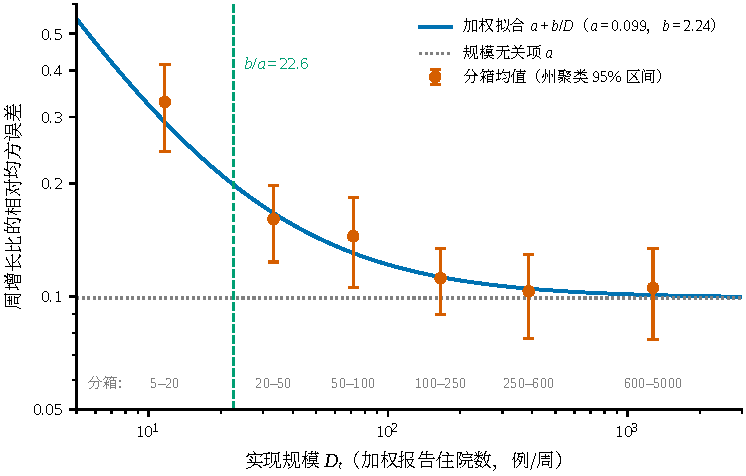
\includegraphics[width=0.8\textwidth]{figures/fig_5_2_early_scale.pdf}
  \caption{流行初期单步预测误差随实现规模 $D_t$ 的变化，共 1,267 个州周。圆点为各分箱均值，画在箱内平均 $D_t$ 处，误差棒为按州聚类重抽的 95\% 区间；曲线为 $a+b/D$ 的拟合，水平虚线为截距 $a$，竖线为经验交叉点 $b/a$。}
  \label{fig:early}
\end{figure}

\subsection{仿射模型的估计}

表~\ref{tab:affine} 汇总主估计与几种估计口径。主估计为 $a=0.0991$（95\% 区间 0.0841--0.1173），$b=2.2434$（1.5019--3.0161），1,500 次重抽中没有一次 $b\leq0$。经验交叉点 $b/a=22.6$ 例/周，区间为 13.7--33.7。用十分位分组均值代替逐观测拟合，交叉点同样为 22.6，说明主估计不依赖分箱方式。

\begin{table}[!tbp]
  \centering
  \caption{流行初期仿射误差模型的估计}
  \label{tab:affine}
  \small
  \begin{tabular}{@{}lccc@{}}
    \toprule
    估计口径 & 截距 $a$ & 斜率 $b$ & 经验交叉点 $b/a$ \\
    \midrule
    可行广义最小二乘（主估计） & 0.0991（0.0841--0.1173） & 2.243（1.502--3.016） & 22.6（13.7--33.7） \\
    十分位分组均值拟合 & 0.1006 & 2.271 & 22.6 \\
    普通最小二乘 & -- & 2.305 & -- \\
    剔除损失最大的 1\% & 0.1077（0.0913--0.1260） & 1.137（0.697--1.661） & 10.6（5.9--17.3） \\
    重抽时重估基准 $\Rbar_{\mathrm{early}}$ & （0.0843--0.1160） & （1.517--2.981） & -- \\
    按周聚类重抽 & （0.0611--0.1317） & （1.473--3.119） & -- \\
    \bottomrule
  \end{tabular}

  \vspace{4pt}
  {\small 注：括号内为 95\% 区间；后两行只改变推断方式，点估计同主估计。各口径下所有重抽的 $b$ 均为正。}
\end{table}

权重的选择只影响效率，不影响一致性。表~\ref{tab:early-bins} 最后一列显示，$\Var(L)/\E(L)^2$ 从最小箱的 5.32 降到最大箱的 0.99，损失的变异系数并不恒定，所以 $1/\hat\mu^2$ 并非最优权重。权重只依赖 $D_t$，与误差项无关，拟合仍然一致；普通最小二乘给出 $b=2.305$，与 2.243 接近。

交叉点对极端值敏感。去掉损失最大的 1\% 观测后，$a$ 升到 0.1077，$b$ 降到 1.137，交叉点降到 10.6。极端损失集中在小规模州周，剔除后斜率下降最多，截距几乎不变。这说明经验交叉点的位置在相当程度上取决于小规模处的尾部行为，下文只把它当作量级。推断方式的两项变化不改变结论。每次重抽都重新估计基准 $\Rbar_{\mathrm{early}}$ 时，$b$ 的 95\% 区间为 1.517--2.981；按周聚类时为 1.473--3.119。州与周两个维度的双向聚类没有做，原因见第~\ref{sec:concl-limits}~节。

\subsection{误差预算与反事实规模}

把平均损失拆开，可以看出扩大规模还剩多少空间。初期样本的平均损失为 0.181，其中截距 $a$ 占 54.6\%，规模项 $b/D_t$ 占 45.1\%，拟合残差占 0.2\%；规模项按 $D_t$ 的调和平均数 27.4 计算。调和平均数接近经验交叉点 22.6，所以两部分大致各占一半，与命题~\ref{prop:average}(ii) 在 $m\approx\mx$ 处的结论一致。

若所有州周的规模都提高到每周 250 例，模型给出的平均损失为 0.107，比现状下降 40.9\%。剩下的 0.107 中，截距 0.0991 占九成以上，继续扩大规模的回报已经很小。实际 $D_t\geq250$ 的 244 个州周，平均损失为 0.104，约为全样本均值的 57\%，与模型给出的 $a+b/250=0.108$ 接近。后一个吻合由拟合机械地决定，大规模观测本身参与了拟合，因此只说明模型在大规模一端没有明显失配，不构成独立证据。

\subsection{与理论情景区间的比较}

经验交叉点 22.6 与理论情景区间处于同一量级。情景参数取 $\Rbar=1.67$，$k\in[0.2,0.5]$\citep{lloydsmith2005superspreading}，$\rho\in[0.0056,0.021]$\citep{zhou2012hospitalizations, tokars2018seasonal}，$v_R\in[0.04,0.08]$。由式~\eqref{eq:var-average}，此时 $A$ 在 1.702--1.967 之间，交叉点 $\mx$ 在 21.3--49.2 之间。报告率很低，$A$ 中的超传播项 $\rho(\Rbar^2+v_R)/k$ 至多约 0.3，$A$ 主要由 $\Rbar$ 决定，交叉点的变化主要来自 $v_R$。

比值落入区间不能当作对结构参数的检验。情景隐含的截距 $v_R/\Rbar^2$ 为 0.0143--0.0287，斜率 $A/\Rbar^2$ 为 0.610--0.705；实证 $a$ 是前者的 3.5--6.9 倍，$b$ 是后者的 3.2--3.7 倍。截距与斜率都被放大了数倍，放大倍数相近，比值才落在区间内。若两者的放大倍数不同，经验交叉点可以远离情景区间，而误差形状本身不变。第~\ref{sec:emp-inflation}~节分析两类放大的来源。

\section{截距与斜率偏大的来源}
\label{sec:emp-inflation}

截距与斜率高于情景隐含值，有两个来源分别作用于斜率和截距。斜率的放大主要来自分母中的报告噪声；截距的放大与环境的时间相关以及 $G_t$ 的口径有关。

\subsection{分母噪声与斜率}

$D_t$ 本身是带二项报告噪声的计数，比真实感染压力 $\rho\Lambda_{t+1}$ 多一层随机性。第四章第~\ref{sec:design-renewal}~节在仿真中已经看到，$D_t$ 偶然偏小时 $G_t$ 被放大，而 $1/D_t$ 是凸函数，对称的分母噪声会抬高平均误差。用 delta 方法展开到 $1/m$ 阶，斜率近似为
\begin{equation}
  b\approx\frac{A+(1-\rho)(\Rbar^2+v_R)\sum_s {w_s}^2}{\Rbar^2},
  \label{eq:b-delta}
\end{equation}
其中 $\sum_s {w_s}^2$ 是式~\eqref{eq:dt-main} 中滞后权重的平方和。式~\eqref{eq:b-delta} 的推导及其成立条件见附录~\ref{app:b-delta}。分子第二项是分母噪声的贡献。住院比例 $\rho$ 很小，$1-\rho$ 接近 1，噪声几乎完整地保留下来；权重越集中，$D_t$ 越接近单周计数，$\sum_s {w_s}^2$ 越大，斜率也越大。分母或自变量含噪时回归系数发生偏移，是测量误差文献中的经典问题\citep{fuller1987measurement, carroll2006measurement}。

式~\eqref{eq:b-delta} 给出一个可检验的预测：改变滞后权重时，斜率应按 $\sum_s {w_s}^2$ 同向变化。表~\ref{tab:lag-weights} 比较三种权重，即主规格（0.65/0.25/0.10，$\sum w^2=0.495$）、只用当周（$\sum w^2=1$）和三周等权（$\sum w^2=0.333$）。实证斜率依次为 2.243、3.134（95\% 区间 2.203--4.067）和 1.926（1.071--2.807），顺序与 $\sum w^2$ 一致。相对主规格，后两者的比值为 1.40 和 0.86；式~\eqref{eq:b-delta} 在情景参数下的预测为 1.44 和 0.86，二者相当接近。三种权重下的 $\Rbar$ 不同（1.48、1.67、1.99），比值的吻合只作方向与量级的对照。

\begin{table}[!tbp]
  \centering
  \caption{三种滞后权重下的实证拟合与情景模拟}
  \label{tab:lag-weights}
  \small
  \begin{tabular}{@{}lccccccc@{}}
    \toprule
    \multirow{2}{*}{规格} & \multirow{2}{*}{$\sum w^2$} & 平均滞后 & \multicolumn{3}{c}{实证} & \multicolumn{2}{c}{情景（$b$）} \\
    \cmidrule(lr){4-6}\cmidrule(l){7-8}
     & & （周） & $a$ & $b$ & $b/a$ & 式~\eqref{eq:b-delta} & 模拟 \\
    \midrule
    只用当周 & 1.000 & 1.00 & 0.0682 & 3.134 & 46.0 & 1.660 & 1.566 \\
    主规格 & 0.495 & 1.45 & 0.0991 & 2.243 & 22.6 & 1.155 & 1.195 \\
    三周等权 & 0.333 & 2.00 & 0.1524 & 1.926 & 12.6 & 0.993 & 0.999 \\
    \bottomrule
  \end{tabular}

  \vspace{4pt}
  {\small 注：情景参数为 $\overline{R}=1.67$，$v_R=0.06$，$k=0.35$，$\rho=0.021$，$A=1.8409$；没有分母噪声时情景斜率为 0.660。模拟以样本均值归一化，每种权重 18,000 个模拟州周。}
\end{table}

情景模拟进一步核对了式~\eqref{eq:b-delta}。情景参数取 $\Rbar=1.67$，$v_R=0.06$，$k=0.35$，$\rho=0.021$，$A=1.8409$。三种权重的预测斜率为 1.155、1.660、0.993，模拟值为 1.195、1.566、0.999。只用当周权重时模拟值低于预测约 6\%，此时分母噪声最大，含噪回归元的稀释、$D_t\geq5$ 的截断与小规模处的高阶余项都更明显，附录~\ref{app:b-delta} 讨论了这三者的方向。图~\ref{fig:noise}a 把实证估计、模拟值与式~\eqref{eq:b-delta} 的直线画在一起，三者随 $\sum w^2$ 同向上升。

在水平上，分母噪声只解释了实证斜率的一部分。没有分母噪声时，情景斜率为 0.660，约为实证值的 29\%；加入二项分母噪声后升到 1.155，约为 51\%。剩余部分的一个可能来源是报告过程的超额离散：若报告数的方差是二项方差的 $\varphi$ 倍，取 $\varphi=1.96$ 时模拟斜率为 2.019，接近实证水平。这只是可能的解释之一，现有数据无法区分超额离散与其他来源，例如各州住院比例的差异。

\subsection{分母噪声不抬高截距}

分母噪声只进入 $1/m$ 阶，不改变截距。情景模拟中主规格、只用当周与三周等权的截距为 0.0202、0.0225、0.0214，几乎不变，都接近 $v_R/\Rbar^2=0.0215$。斜率被放大而截距不变，于是 $b/a$ 被推高。主规格的模拟比值为 59.2，而真实的 $A/v_R$ 只有 30.7。用经验交叉点估计 $\mx$ 因而会系统性偏大。实证中 $b/a$ 没有偏大到这一程度，是因为实证截距也被放大了，两种放大部分抵消。

\subsection{截距随回溯滞后上升}

截距的放大另有来源。表~\ref{tab:lag-weights} 中实证截距随平均回溯滞后单调上升，平均滞后为 1.0、1.45、2.0 周时，$a$ 分别为 0.0682、0.0991、0.1524，都远高于情景隐含的 0.014--0.029（图~\ref{fig:noise}b）；模拟中截距不随滞后变化。这一模式与第四章式~\eqref{eq:mse-decomp} 的条件偏差项一致。真实的 $R_t$ 有时间相关，分母越陈旧，$\mu_t/D_t$ 偏离 $\Rbar$ 越远，偏差项越大。$G_t$ 跨两代左右，代际之间的环境波动叠加，也会放大与规模无关的部分。两种机制都作用于截距，现有数据无法把它们分开。

\begin{figure}[!tbp]
  \centering
  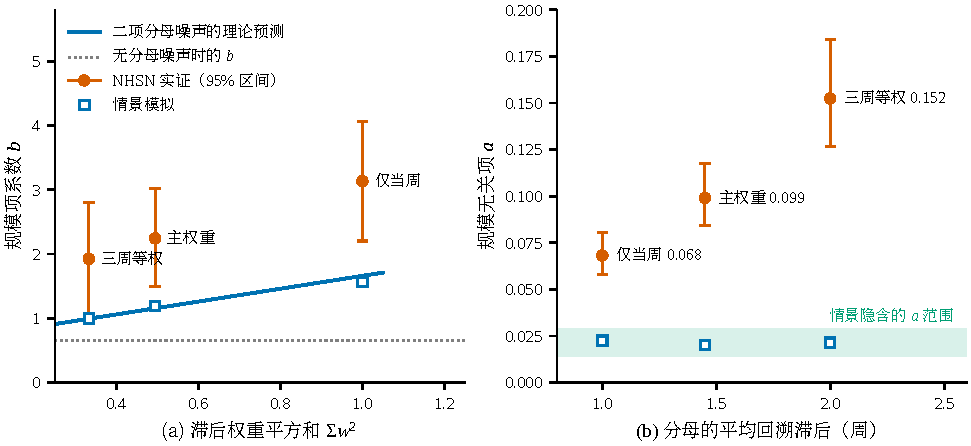
\includegraphics[width=\textwidth]{figures/fig_5_3_denominator_noise.pdf}
  \caption{滞后权重对拟合系数的影响。（a）规模项系数 $b$ 与滞后权重平方和 $\sum w^2$ 的关系。圆点为三种权重的实证估计及 95\% 区间，方块为情景模拟值，斜线为二项分母噪声的一阶近似，水平虚线为没有分母噪声时的 $b$。（b）截距 $a$ 与分母平均回溯滞后的关系，阴影为情景隐含的截距范围 0.014--0.029。}
  \label{fig:noise}
\end{figure}

三种滞后权重下规模项都为正，误差形状稳定。经验交叉点则随权重在 12.6--46.0 之间变化，变化方向由斜率与截距的相反走势共同决定，权重越集中，斜率越大、截距越小，交叉点越大。经验交叉点描述的是 $G_t$ 这一统计量的误差结构，它随规模测度的选择而移动，不能当作 $A/v_R$ 的估计。

\section{达峰期的误差结构}
\label{sec:emp-peak}

\subsection{基准偏移}

流行达峰后，阶段均值本身发生变化。取三个流行季的全国峰值周（2022 年 12 月 3 日、2023 年 12 月 30 日、2025 年 2 月 8 日）及其后 7 周，共 1,220 个州周，平均增长比降到 $\Rbar_{\mathrm{peak}}=0.8075$，标准差 0.3048。平均增长比小于 1，说明住院数在这一阶段平均每周下降约两成。若继续用初期均值 1.6706 作基准，各箱的平均损失都在 0.29--0.31 之间，看不出随规模下降。

在固定基准下，损失可以拆成两块：基准偏移造成的常数偏差，以及箱内围绕峰期均值的波动。常数偏差为
\begin{equation}
  \frac{(\Rbar_{\mathrm{early}}-\Rbar_{\mathrm{peak}})^2}{\Rbar_{\mathrm{early}}^2}=0.2669,
  \label{eq:peak-bias}
\end{equation}
它与规模无关，相当于在式~\eqref{eq:mse-decomp} 的条件偏差项中加入了一个阶段转换的偏移。表~\ref{tab:peak-bins} 与图~\ref{fig:peak} 给出分箱结果。偏差项占总损失的 88.9\%，从最小箱的 59.5\% 升到最大箱的 94.8\%。规模越大，箱内波动越小，偏差项的占比越高。除最小箱外，峰期损失是同箱初期损失的 1.8--2.9 倍；最小箱只有 33 个州周，峰期的小规模州周较少，其比值 0.91 不稳定。

\begin{table}[!tbp]
  \centering
  \caption{达峰期以初期均值为基准时的分箱误差分解}
  \label{tab:peak-bins}
  \small
  \begin{tabular}{@{}lccccccc@{}}
    \toprule
    $D_t$ 分箱 & 州周数 & 总损失 & 偏差项 & 箱内波动 & 偏差占比（\%） & 初期损失 & 峰期/初期 \\
    \midrule
    $[5,20)$ & 33 & 0.300 & 0.178 & 0.122 & 59.5 & 0.329 & 0.91 \\
    $[20,50)$ & 140 & 0.293 & 0.227 & 0.066 & 77.6 & 0.160 & 1.82 \\
    $[50,100)$ & 162 & 0.312 & 0.270 & 0.042 & 86.6 & 0.145 & 2.16 \\
    $[100,250)$ & 312 & 0.305 & 0.276 & 0.029 & 90.5 & 0.112 & 2.73 \\
    $[250,600)$ & 311 & 0.300 & 0.277 & 0.023 & 92.4 & 0.103 & 2.90 \\
    $[600,5000)$ & 262 & 0.292 & 0.277 & 0.015 & 94.8 & 0.105 & 2.77 \\
    \bottomrule
  \end{tabular}

  \vspace{4pt}
  {\small 注：峰期为各季全国峰值周及其后 7 周，共 1,220 个州周；基准为初期均值 1.6706。}
\end{table}


\begin{figure}[!tbp]
  \centering
  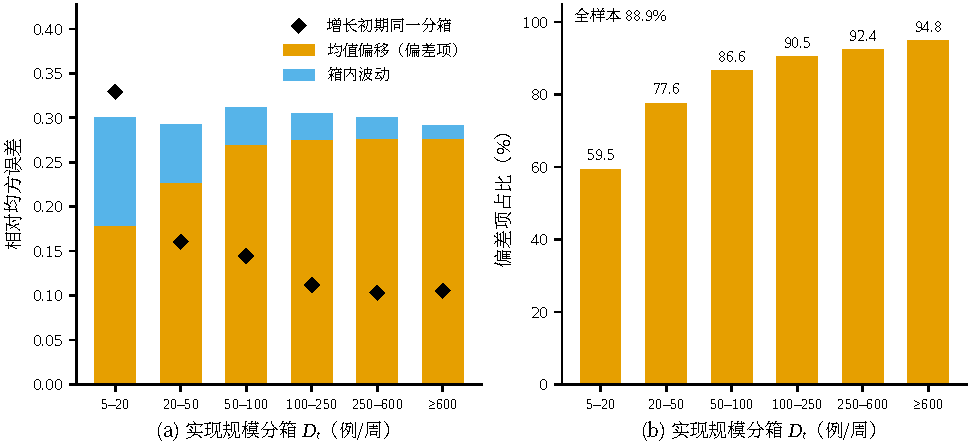
\includegraphics[width=\textwidth]{figures/fig_5_4_peak_decomp.pdf}
  \caption{达峰期（峰值周及其后 7 周）以流行初期均值为基准时的误差分解。（a）各规模箱的平均损失，分为基准偏移造成的偏差项与箱内波动，菱形为同一分箱在流行初期的平均损失；（b）偏差项在各箱损失中的占比。}
  \label{fig:peak}
\end{figure}

\subsection{阶段自身基准下的规模效应}

改用峰期自身均值作基准后，规模效应重新出现，$a=0.0665$（95\% 区间 0.0467--0.0897），$b=7.927$（5.424--11.225），交叉点 119.2（64.0--225.9），平均损失 0.142。峰期的误差仍然呈“常数加规模反比”的形状，规模项在峰期依然有用。

峰期的 $b$ 不能直接与初期的 2.243 比较。式~\eqref{eq:loss} 以阶段均值的平方归一化，峰期均值只有初期的一半左右，归一化分母小了约四倍，斜率因而被机械地放大。统一用 $\Rbar_{\mathrm{early}}$ 归一化后，峰期斜率为 1.852，低于初期的 2.243；不归一化时为 5.169 对 6.261。在同一样本上做联合回归，阶段交互项的普通最小二乘估计为 $-0.92$，95\% 区间 $-2.33$--$0.59$，包含零。因此，达峰期规模仍然有用，但没有证据表明它比初期更有用或更没用。

达峰期结果揭示了误差的另一种来源。阶段转换时，基准的偏移量远大于规模项，用旧基准预测新阶段，规模再大也无法降低误差。监测上的对应做法是换用能够跟踪基准变化的模型，同时继续维持病例规模，前者处理偏差项，后者处理规模项。第六章用时变基准与 FluSight 集成预测考察第一点。

\section{填报制度变化}
\label{sec:emp-policy}

填报制度的变化提供了另一类证据。按命题~\ref{prop:reporting}，报告率下降会增加方差；若填报率下降只是均匀地稀疏了病例，$G_t$ 的离散程度应按可预测的幅度上升。表~\ref{tab:policy} 与图~\ref{fig:policy} 比较三期 $G_t$ 的分布。

从第一期到第二期，$G_t$ 的标准差从 0.624 升到 1.823，增加 192\%；第三期回到 0.649。稳健离散度几乎不动，四分位距依次为 0.638、0.594、0.652，第二期反而略低；中位绝对偏差为 0.298、0.299、0.292。偏度从 3.29 升到 14.98，再回到 2.68；最大值从 12.7 升到 33.9。第 10 百分位数从 0.468 降到 0.199，左尾也在扩张。两端尾部都变厚，而分布中部不变。

\begin{figure}[!tbp]
  \centering
  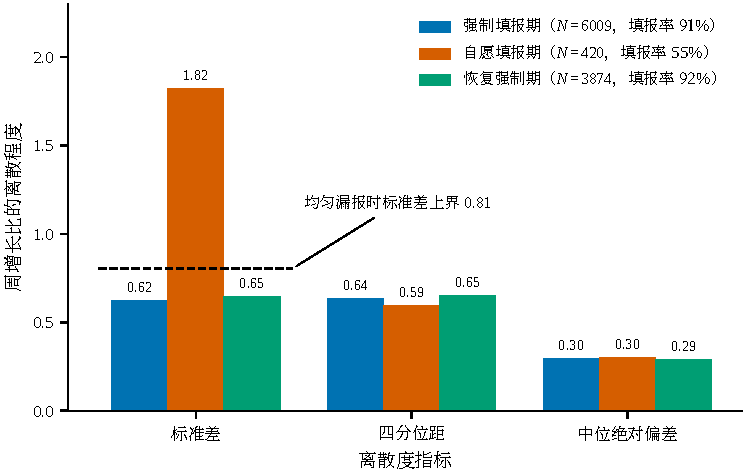
\includegraphics[width=0.8\textwidth]{figures/fig_5_5_reporting_policy.pdf}
  \caption{三个填报制度期内周增长比 $G_t$ 的离散程度。柱上数字为指标值；虚线为填报率从 91.1\% 降至 54.6\% 时，若漏报在医院间均匀发生，第二期标准差可能达到的上限。}
  \label{fig:policy}
\end{figure}

均匀稀疏给出的上限可以直接计算。若填报医院的减少相当于把每家医院的病例按相同比例抽稀，规模缩小到原来的 $54.59/91.11$，按规模项与 $1/m$ 成正比且忽略环境项，标准差最多放大到
\begin{equation}
  0.624\times\sqrt{91.11/54.59}=0.806,
  \label{eq:sd-bound}
\end{equation}
即 1.29 倍。实际放大了 2.92 倍，而且只有标准差放大，分位数指标不变。离散程度的扩张因此来自少数极端周，例如部分医院时报时不报造成的跳变：某周填报医院骤减，住院数随之骤降，$G_t$ 落入左尾；次周恢复填报，$G_t$ 落入右尾。整体噪声并没有均匀增加。第二期缺失的 36 个州周按 0 计入，也会制造这类跳变。

两项对照排除了两个明显的混杂。第二期覆盖 5--10 月，多为非流行季，因此先检查季节构成。只取 10 月至次年 3 月的周，第一期与第三期的标准差为 0.652 和 0.706，第二期（仅 2024 年 10 月，55 个州周）为 4.79，扩张仍然存在，但第二期的样本很少。填报率的连续变化同样不能解释扩张：以 2022 年 10 月 1 日为界把第一期分为两段，平均填报率由 87.8\% 升到 93.7\%，标准差为 0.628 和 0.620，几乎不变。强制填报下填报率的小幅变化不影响离散程度，自愿填报带来的变化是结构性的。

第二期离散度的扩张与命题~\ref{prop:reporting} 只有定性联系。报告率下降确实增加了方差，但第二期的主要变化是填报行为的结构性扰动，无法用 $\rho$ 的变化定量解释。对监测数据质量的评估而言，标准差对这类扰动最敏感，四分位距与中位绝对偏差则反映整体噪声水平，两类指标并用可以区分结构性扰动与均匀漏报。

\section{本章小结}
\label{sec:emp-summary}

本章在美国 51 个辖区的流感住院周报上检验了第三章的误差形状。流行初期 1,267 个州周的相对均方误差随实现规模下降并趋于平缓。可行广义最小二乘估计的截距为 0.0991，斜率为 2.243，所有重抽的斜率都为正。经验交叉点为 22.6 例/周，与理论情景区间 21.3--49.2 处于同一量级。平均损失中截距与规模项大致各占一半。把规模提高到每周 250 例，模型给出的损失下降约四成，此后截距占九成以上。

截距与斜率都是情景隐含值的三倍以上，比值的吻合因此不能作为结构参数的检验。滞后权重的比较表明，分母中的二项报告噪声按 $\sum w^2$ 抬高斜率而不改变截距，其预测的相对变化与实证吻合。二项噪声只能解释斜率水平的一半左右。截距随分母的回溯滞后单调上升，与环境的时间相关和 $G_t$ 的口径一致。经验交叉点随规模测度在 12.6--46.0 之间移动，只能作量级参考。

达峰期以初期均值为基准时，88.9\% 的损失来自基准偏移，规模效应被掩盖；换用峰期自身基准后规模项重新为正，阶段间的斜率差异不显著。自愿填报期 $G_t$ 的标准差扩张 192\%，稳健离散度不变，扩张来自少数极端周，超出均匀稀疏所能解释的幅度。第六章检验这些结论在替代设定、空间汇总与外部数据下是否保持。

\chapter{稳健性与外部验证}
\label{chap:robust}

第五章的主结论有三项。流行初期的误差随规模下降并趋于常数，规模项显著为正。经验交叉点与理论情景区间同量级，但截距与斜率都被放大。阶段转换时，基准偏移掩盖规模效应。主分析有五项设定可能影响这些结论。规模与预测对象来自同一序列，基准用到了整个窗口的数据，且在窗口内固定不变。分析单元是单个州，数据只有一种病和一个报告系统。本章逐项改变这些选择。第~\ref{sec:rob-forest}~节先汇总各规格下的经验交叉点。第~\ref{sec:rob-iv}~节至第~\ref{sec:rob-tv}~节依次改变规模测度、基准的信息集和基准的时变性。第~\ref{sec:rob-pool}~节用全国汇总序列考察空间汇总。第~\ref{sec:rob-external}~节引入两组外部数据。第~\ref{sec:rob-discussion}~节讨论结果对监测工作的含义及其与已有研究的关系。

\section{各规格的汇总}
\label{sec:rob-forest}

图~\ref{fig:forest} 汇总了第五章与本章各规格下的经验交叉点 $b/a$。所有规格的规模项都为正，凡给出区间的规格，区间都不含零。交叉点则在 10.6--124.7 之间变化，跨越一个数量级。NHSN 数据的各规格大多落在 10--75 之间，外部数据的交叉点更大。变化的方向有规律可循。分母噪声越大、基准对小规模越敏感，斜率越大，交叉点越靠右；剔除极端值则把交叉点推向左侧。规模项为正这一定性结论在所有规格下保持，交叉点的具体数值则取决于规格，只能作为量级参考。

\begin{figure}[!tbp]
  \centering
  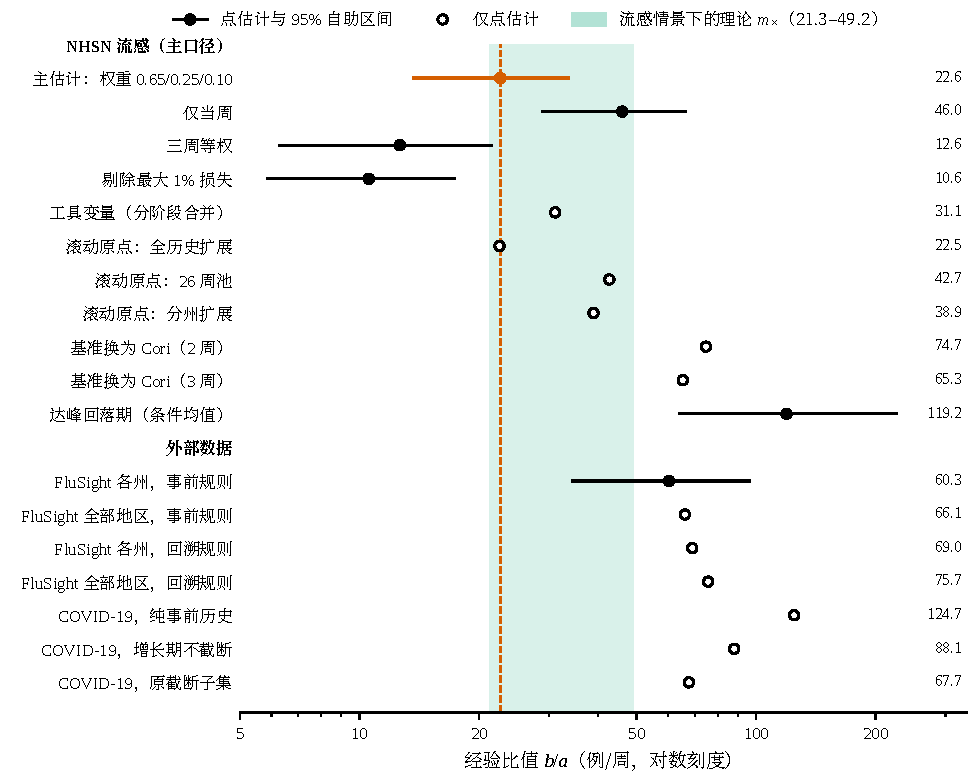
\includegraphics[width=\textwidth]{figures/fig_6_1_mx_forest.pdf}
  \caption{各规格下的经验交叉点 $b/a$。横线为 95\% 区间（只有部分规格提供），阴影为理论情景区间 21.3--49.2，竖直虚线为主估计 22.6，右侧列出点估计。上部为 NHSN 数据的不同规格，下部为外部数据。}
  \label{fig:forest}
\end{figure}

\section{替代性规模测度与工具变量}
\label{sec:rob-iv}

主分析中的 $D_t$ 与 $C_{t+1}$ 来自同一序列，同期测度可能带来两类问题。$D_t$ 含报告噪声，作为回归元时会造成衰减偏误\citep{fuller1987measurement, carroll2006measurement}；规模还可能与当期传播水平相关，规模大的州周恰好处在传播较快的时期。两种情形下 $1/D_t$ 都与回归误差相关，普通最小二乘与可行广义最小二乘都不一致。

工具变量法要求工具与 $1/D_t$ 相关，而与误差项无关。这里取滞后 3--5 周的规模作为 $1/D_t$ 的工具，在流行季内合并样本上做两阶段最小二乘\citep{wooldridge2010econometric}。各州的规模在季内平稳变化，三到五周前的规模与当前规模高度相关；滞后足够长时，旧规模中的报告噪声与当前分母中的噪声相互独立。合并样本要求每个州周都有完整的滞后，共 1,051 个州周，与主样本不同，比较应在同一样本上进行。区间由 10,000 次按州聚类的重抽给出。

表~\ref{tab:iv} 列出合并样本与分季的结果。合并样本的 $b_{\mathrm{iv}}=2.53$（95\% 区间 1.11--4.11），同一样本上的普通最小二乘为 1.35。两者之差的区间为 0.30--2.11，不含零，对应的交叉点为 31.1。改用子样本自身的均值作基准，$b_{\mathrm{iv}}=2.85$（1.32--4.55），交叉点 35.3。第一阶段 $F$ 统计量为 1,147.1，按州聚类后为 312.9，远高于弱工具的常用门槛 10。分季来看，三个流行季的 $b_{\mathrm{iv}}$ 都为正，区间都不含零，点估计都高于同季的普通最小二乘。差值只在 2024--25 季的区间不含零。另两季的区间含零，单季样本只有 273--420 个州周，精度有限。

\begin{table}[!tbp]
  \centering
  \caption{以滞后规模为工具的两阶段最小二乘估计}
  \label{tab:iv}
  \small
  \begin{tabular}{@{}lcccccc@{}}
    \toprule
    样本 & 州周数 & $b_{\mathrm{iv}}$（95\% 区间） & $b_{\mathrm{ols}}$ & 差值的 95\% 区间 & $b_{\mathrm{iv}}/a_{\mathrm{iv}}$ & 聚类 $F$ \\
    \midrule
    2022--23 季 & 273 & 3.28（0.90--6.47） & 1.89 & $-0.15$--3.89 & 60.2 & 94.5 \\
    2023--24 季 & 358 & 2.19（0.65--4.31） & 1.68 & $-0.55$--1.74 & 58.5 & 119.4 \\
    2024--25 季 & 420 & 3.61（0.73--7.23） & 1.83 & 0.01--3.47 & 30.5 & 76.8 \\
    合并（季内均值） & 1,051 & 2.53（1.11--4.11） & 1.35 & 0.30--2.11 & 31.1 & 312.9 \\
    合并（子样本均值） & 1,051 & 2.85（1.32--4.55） & 1.46 & 0.43--2.41 & 35.3 & 312.9 \\
    \bottomrule
  \end{tabular}

  \vspace{4pt}
  {\small 注：工具为滞后 3--5 周的规模；区间由 10,000 次按州聚类的重抽得到；聚类 $F$ 为按州聚类的第一阶段 $F$ 统计量。}
\end{table}

$b_{\mathrm{iv}}$ 高于普通最小二乘，与回归元含噪造成的衰减偏误方向一致。工具变量斜率高于普通最小二乘，与第五章第~\ref{sec:emp-inflation}~节并不矛盾。分母噪声通过两条途径影响斜率：进入 $G_t$ 时抬高小规模处的损失，使斜率变大；进入回归元 $1/D_t$ 时稀释斜率，使斜率变小。式~\eqref{eq:b-delta} 描述前一条途径，工具变量处理的是后一条途径。排除限制要求滞后规模只通过当前规模影响损失，这一条件无法检验；若滞后规模与当前的传播阶段相关，工具变量估计仍有偏。因此工具变量结果只说明，在替代性规模测度下规模项保持为正。

\section{事前基准}
\label{sec:rob-exante}

主分析的基准 $\Rbar_{\mathrm{early}}$ 用整个窗口的数据计算，属于回顾性口径。实时监测中，当周只能使用过去的信息。若规模效应只是回顾性基准的产物，换用事前基准后应当消失。这里考察三种只含过去信息的基准。全部州的历史扩张窗取当周之前所有州周增长比的均值。26 周滚动池取当周之前 26 周内所有州周的均值。逐州扩张窗取同一州此前各周的均值。

表~\ref{tab:exante} 的上半部分给出结果。三种事前基准下误差整体上升，截距 $a$ 在 0.222--0.406 之间，是主估计的 2.2--4.1 倍；斜率 $b$ 在 9.16--13.27 之间，所有重抽的 $b$ 都为正。交叉点为 22.5--42.7，仍与理论情景区间同量级。截距在平均损失中的份额随口径在 39\%--55\% 之间移动。

\begin{table}[!tbp]
  \centering
  \caption{事前基准与时变基准下的误差}
  \label{tab:exante}
  \small
  \begin{tabular}{@{}lccccc@{}}
    \toprule
    基准 & 州周数 & 平均损失 & 截距 $a$ & 斜率 $b$（95\% 区间） & $b/a$ \\
    \midrule
    \multicolumn{6}{@{}l}{事前基准} \\
    全部州历史扩张窗 & 1,267 & -- & 0.406 & 9.16（5.82--12.88） & 22.5 \\
    26 周滚动池 & 1,267 & -- & 0.222 & 9.46（6.76--12.81） & 42.7 \\
    逐州扩张窗 & 1,260 & -- & 0.341 & 13.27（9.14--18.29） & 38.9 \\
    \midrule
    \multicolumn{6}{@{}l}{时变基准} \\
    阶段均值（主估计） & 1,267 & 0.181 & 0.0991 & 2.24（1.50--3.02） & 22.6 \\
    Cori 滑动窗（1 周） & 1,197 & 0.436 & -- & -- & -- \\
    Cori 滑动窗（2 周） & 1,244 & 0.288 & 0.0812 & 6.06 & 74.7 \\
    Cori 滑动窗（3 周） & 1,251 & 0.249 & 0.0763 & 4.98 & 65.3 \\
    朴素预测（下周等于本周） & 1,267 & 0.637 & -- & -- & -- \\
    \bottomrule
  \end{tabular}

  \vspace{4pt}
  {\small 注：每种基准的损失都以该基准自身的预测值归一化；“--”表示未作相应计算。}
\end{table}

截距的上升有明确来源。事前基准只能用过去的增长比外推，流行初期增长比本身在逐周变化，过去的均值与当周的阶段水平之间存在系统差距。按第四章式~\eqref{eq:mse-decomp}，这一差距进入条件偏差项，与规模无关，因而表现为截距上升。斜率同样上升，但规模项为正的结论不变。事前基准解决了基准的前视问题，没有解决窗口划定本身用到事后信息的问题，后者在第~\ref{sec:concl-limits}~节讨论。

\section{时变基准}
\label{sec:rob-tv}

阶段均值基准在整个窗口内固定不变。若改用逐周更新的基准，规模效应是否仍然存在，截距能否降低，是第五章达峰期结果留下的问题。这里用 \citet{cori2013new} 的滑动窗口方法估计 $R_t$，以最近 1、2、3 周的报告数之和除以对应的感染压力之和，作为下一周增长比的预测。作为对照，朴素预测直接以本周病例数预测下周。

表~\ref{tab:exante} 的下半部分给出平均损失。阶段均值基准为 0.181，Cori 滑动窗随窗宽由 1 周增至 3 周，从 0.436 降到 0.249，朴素预测为 0.637。对 Cori 基准的损失拟合式~\eqref{eq:affine}，2 周窗 $a=0.0812$，$b=6.064$，交叉点 74.7；3 周窗 $a=0.0763$，$b=4.984$，交叉点 65.3。两种窗宽的截距都低于阶段均值基准的 0.0991，斜率则是后者的 2--3 倍。

图~\ref{fig:baselines} 按规模分箱比较四种基准。按各自预测值归一化时（图~\ref{fig:baselines}a），$D_t<100$ 的三箱中阶段均值基准的损失最低，Cori 2 周窗在最小箱为 0.658，是阶段均值基准 0.329 的两倍。$D_t\geq100$ 的三箱中两种 Cori 基准都略低于阶段均值基准，例如 $[100,250)$ 箱的 0.090 和 0.087 对 0.112。朴素预测在所有箱中损失最高。统一以 $\Rbar_{\mathrm{early}}$ 归一化、只用 Cori 2 周窗可用的 1,244 个州周时（图~\ref{fig:baselines}b），Cori 2 周窗的平均损失为 0.223，朴素预测为 0.274；在最大箱中朴素预测降到 0.064，低于阶段均值基准的 0.105。

\begin{figure}[!tbp]
  \centering
  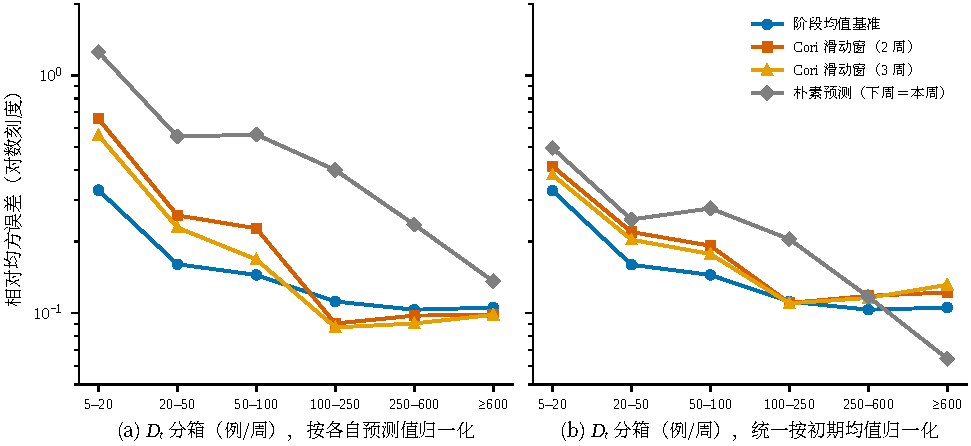
\includegraphics[width=\textwidth]{figures/fig_6_2_baselines.pdf}
  \caption{流行初期四种预测基准在各规模分箱上的相对均方误差，纵轴为对数刻度。（a）每种基准的损失以其自身预测值归一化，各基准使用各自可计算的样本；（b）四种基准的损失统一以初期均值 $\overline{R}_{\mathrm{early}}$ 归一化，样本限于 Cori 2 周窗可计算的 1,244 个州周。}
  \label{fig:baselines}
\end{figure}

分箱结果说明了截距的构成。时变基准用近期数据估计 $R_t$，自身就是一个带抽样噪声的比值，规模小时噪声大，斜率因此更陡。规模大时抽样噪声可以忽略，时变基准能跟踪各州各周增长水平的变化，误差低于固定基准。大规模处的误差下降意味着，阶段均值基准的截距中有一部分来自可由近期数据预测的增长水平变化。这部分误差不属于规模无法消除的环境方差。这与第五章截距随回溯滞后上升的结果一致，$R_t$ 的时间相关使近期数据含有当期传播水平的信息。时变基准降低截距的幅度有限，最大箱中 Cori 2 周窗仍有 0.098，截距不会因换用时变基准而消失。

\section{空间汇总}
\label{sec:rob-pool}

第三章式~\eqref{eq:pooling} 表明，汇总 $J$ 个辖区后环境底板降为 $v_R\bar c+v_R(1-\bar c)/J$，降幅取决于辖区间环境波动的平均相关 $\bar c$。全国加总序列提供了一个检验。三个流行初期窗口中，全国序列共 28 周，平均规模约 6,662 例/周，平均增长比 1.539，平均损失 0.0348，中位数 0.0115。按主估计 $b=2.243$，规模项 $b/D$ 约为 0.0003，可以忽略，全国序列的损失几乎全部是环境底板。

以州级截距 0.0991 作为单辖区的底板，比值 $0.0348/0.0991=0.351$。代入式~\eqref{eq:pooling}，$J=51$ 时
\begin{equation}
  \bar c+\frac{1-\bar c}{51}=0.351 ,
  \label{eq:cbar}
\end{equation}
解得 $\bar c\approx0.34$。各州的环境波动只有约三分之一是全国共同的，其余部分在汇总中相互抵消。若各州完全同步（$\bar c=1$），汇总不会降低底板；若完全独立（$\bar c=0$），底板会降到州级的 1/51。实际降幅介于两者之间。

这一推算较为粗略。全国序列只有 28 周，平均损失的抽样误差较大。州级截距 0.0991 本身被分母噪声和 $G_t$ 的口径放大，第五章已说明它高于真实的 $v_R/\Rbar^2$。全国序列的平均增长比 1.539 也不同于州级的 1.6706，两者归一化的尺度不同。$\bar c\approx0.34$ 只能当作量级。在方向上，汇总确实把环境底板降到州级的三分之一左右，与命题~\ref{prop:allocation} 的时间方向结论相互补充。时间上增加期数与空间上增加辖区，都能降低平均传播水平估计的误差。两者的效果分别受时间相关与空间相关的限制。

\section{外部数据}
\label{sec:rob-external}

\subsection{FluSight 集成预测}

前述分析都使用以阶段均值为核心的简单基准。实际的流感预测由多个团队的模型集成给出。FluSight 是美国疾病控制与预防中心组织的流感住院前瞻预测，这里使用其 2022--23 季的集成预测\citep{mathis2024evaluation}，相关评价框架见文献\citep{reich2019accuracy, cramer2022evaluation}。集成预测给出下一周住院数的预测值 $\widehat Y$。主口径以 $\widehat Y$ 作为规模测度并据此筛选样本，筛选只用事前信息。

以 $\widehat Y\geq5$ 筛选州级样本（$N=1{,}177$），对相对误差平方拟合式~\eqref{eq:affine}，得到 $a=0.1295$（95\% 区间 0.1020--0.1633），$b=7.805$（5.358--10.526），交叉点 60.3（34.5--95.9）。表~\ref{tab:external} 列出另外三种筛选口径，交叉点为 66.1、69.0 和 75.7。集成预测的截距与阶段均值基准接近，斜率是后者的三倍以上，交叉点相应更大。

把集成预测在各流行阶段内的相对均方误差拆成均值偏差平方与阶段内方差两部分，均值偏差平方在上升期（$N=216$）占 32.3\%，在峰期（$N=206$）占 15.5\%，在回落期（$N=755$）占 1.5\%。第五章中阶段均值基准在达峰期的偏差占比为 88.9\%。集成预测在峰期能较好地跟踪阶段变化，偏差占比低得多，上升期的偏差占比最高，与预测模型对增长起点反应滞后的情形相符，现有分解不足以确定其原因。两组数字来自不同的模型、季节和样本，只能作方向性参照。

\subsection{欧洲 COVID-19 早期序列}

第二组外部数据是欧洲 11 国 2020 年 2--4 月的 2019 冠状病毒病序列\citep{flaxman2020estimating}，单元为国家。三种口径的结果列于表~\ref{tab:external}。只用过去信息构造基准时，$N=404$，$b=33.92$（14.60--74.99），交叉点 124.7；只取增长期为 88.1，截断子样本为 67.7。三种口径的规模项都为正，交叉点都高于 NHSN 主估计。

\begin{table}[!tbp]
  \centering
  \caption{外部数据的仿射误差模型估计}
  \label{tab:external}
  \small
  \begin{tabular}{@{}llcccc@{}}
    \toprule
    数据 & 口径 & 单元数 & 截距 $a$ & 斜率 $b$（95\% 区间） & $b/a$ \\
    \midrule
    FluSight 2022--23 & 州，事前 $\widehat Y\geq5$ & 1,177 & 0.129 & 7.80（5.36--10.53） & 60.3 \\
     & 全部地区，事前 & 1,203 & 0.122 & 8.07 & 66.1 \\
     & 州，事后 $C\geq5$ & 1,137 & 0.124 & 8.52 & 69.0 \\
     & 全部地区，事后 $C\geq5$ & 1,163 & 0.116 & 8.81 & 75.7 \\
    \midrule
    欧洲 COVID-19 & 纯事前基准 & 404 & 0.272 & 33.92（14.60--74.99） & 124.7 \\
     & 仅增长期 & 318 & 0.210 & 18.53（7.13--44.10） & 88.1 \\
     & 截断子样本 & 307 & 0.189 & 12.76（7.25--20.01） & 67.7 \\
    \bottomrule
  \end{tabular}

  \vspace{4pt}
  {\small 注：FluSight 的单元为州周，聚类单元为州；欧洲 COVID-19 的观测按国家与时间索引，聚类单元为国家。}
\end{table}

COVID-19 序列的交叉点更大，与该序列更高的平均增长比相符。三种口径的平均增长比在 2.9--3.5 之间，按式~\eqref{eq:var-average}，规模项 $A$ 随 $\Rbar$ 增大。2020 年初各国检测能力变化较快，报告率不稳定也可能抬高斜率。两组外部数据的病种、预测方法和报告系统都与 NHSN 不同，交叉点不宜直接比较大小。外部数据支持的结论是定性的：误差中存在随规模下降的成分，且在规模达到数十至一百余例后趋于平缓。

\section{讨论}
\label{sec:rob-discussion}

\subsection{对监测工作的含义}

全文的核心区分是估计目标。同一份病例数据，用来判断本周是否在增长，与用来估计一段时期的平均传播水平，对规模的需求相差很大。前者属于目标Ⅰ，方差随规模趋于零，第四章第~\ref{sec:design-test}~节的计算表明，要稳定检出 15\% 的增长，所需规模约为交叉点的十倍。后者属于目标Ⅱ，规模超过 $\mx$ 以后误差主要来自环境波动，扩大病例捕获的回报迅速变小。

由此可以提出双轨监测的思路。预警类问题对应目标Ⅰ，规模越大越好，资源应投向报告及时、覆盖完整的单元。趋势类问题对应目标Ⅱ，规模达到交叉点的量级后，更有效的做法是增加观测期数，或汇总多个辖区。命题~\ref{prop:allocation} 与式~\eqref{eq:pooling} 分别给出时间与空间两个方向的收益，第~\ref{sec:rob-pool}~节的全国序列把环境底板降到州级的三分之一左右。

阶段转换时的误差需要另一类对策。达峰期以初期均值为基准时，88.9\% 的损失来自基准偏移，规模再大也无济于事；换用阶段自身基准后，规模项重新为正。时变基准在大规模处降低了误差，FluSight 集成预测在峰期的偏差占比只有 15.5\%，两者都表明能跟踪阶段变化的模型可以压低偏差项。在流行阶段转换时，应优先更新基准模型，同时维持足以控制规模项的病例数。

数据质量的监控也可以从第五章得到启示。自愿填报期 $G_t$ 的标准差大幅扩张，四分位距与中位绝对偏差几乎不变，扰动集中在少数极端周。这类结构性扰动比均匀漏报更难处理。用稳健离散度监控整体噪声，用标准差与偏度识别结构性扰动，两类指标并用，可以较早地发现填报行为的变化。

\subsection{与已有研究的关系}

Parag 等的信息论结果针对当期再生数，Fisher 信息随病例数线性增长\citep{parag2022quantifying, parag2022fundamental}，这与目标Ⅰ的结论一致。本文补充的是目标Ⅱ：环境方差 $v_R$ 给出一个规模无法突破的底板，交叉点 $\mx$ 把这一底板换算成具体的病例数。生态学区分环境随机性与人口随机性\citep{engen1998demographic, rohani2002determinism}，前者影响整个种群，后者随种群规模增大而平均掉；第三章的方差分解在监测设计中给出了这一区分的对应。

预测评价文献通常按地区或时期报告误差\citep{reich2019accuracy, cramer2022evaluation}。本章的 FluSight 结果表明，集成预测的误差同样含有随规模下降的成分与不随规模下降的底板。按相对误差比较不同规模的地区时，小规模地区的误差偏高有一部分来自规模项，这部分与模型优劣无关。把规模作为协变量纳入预测评价，可以把模型差异与规模差异分开。

\section{本章小结}
\label{sec:rob-summary}

本章在替代规格、空间汇总与外部数据下检验了第五章的结论。以滞后规模为工具的两阶段最小二乘给出 $b_{\mathrm{iv}}=2.53$，高于同一样本的普通最小二乘，方向与衰减偏误一致。三种事前基准下截距上升到主估计的 2--4 倍，规模项仍然为正。Cori 滑动窗口基准在小规模处误差更大，在大规模处略低于阶段均值基准，说明截距中有一部分是可由近期数据预测的增长水平变化。全国汇总序列的损失约为州级截距的三分之一，粗略推算的州间环境相关约为 0.34。FluSight 集成预测与欧洲 COVID-19 序列中规模项都为正，交叉点为 60.3--124.7。

所有规格下规模项都为正，经验交叉点则在 10.6--124.7 之间变化。规模的收益随规模递减、存在环境底板这一定性结论是稳健的；交叉点的具体数值依赖规格、病种与预测方法，只能作为量级参考。这些结果对监测设计的含义已在第~\ref{sec:rob-discussion}~节讨论，第七章将其归纳为实践建议。

\chapter{结论与展望}
\label{chap:conclusion}

本文研究病例规模在疫情监测中的收益边界。出发点是一个常被默认的判断：报告病例越多，对传播水平的估计越准确。第三章到第六章表明，这一判断对一类估计目标成立，对另一类估计目标只在一定规模以内成立，边界的位置可以折算成病例数，并在住院监测数据中观察到对应的误差形状。本章归纳主要结论，说明研究的局限，并提出监测实践的建议与后续研究方向。

\section{主要结论}
\label{sec:concl-main}

第一，规模的收益取决于估计目标。在负二项传播与二项报告的单代模型下，若目标是当期再生数 $R_t$，估计量 $C_t/(\rho n)$ 是无偏的极大似然估计。它在任意有限规模下的效率都达到最优，方差随规模趋于零（命题~\ref{prop:current}）。若目标是跨期平均再生数 $\Rbar$，方差为 $v_R+A/m$，规模只能消除第二项，环境方差 $v_R$ 构成规模无法突破的底板（命题~\ref{prop:average}）。两类目标使用同一份数据，对规模的需求相差一个数量级以上。

第二，环境底板可以折算成病例数。交叉点 $\mx=A/v_R$ 是规模项等于环境项时的预计报告规模，规模达到 $\mx$ 时误差的一半来自环境波动，扩大规模至多再降低一半误差。对住院监测，$A$ 中的超传播项很小，交叉点主要由 $\Rbar$ 与 $v_R$ 决定；按文献给出的情景参数，交叉点为每期 21.3--49.2 例报告。报告率很低时，扩大覆盖与提高报告率的边际效果几乎相同（命题~\ref{prop:reporting}）。

第三，方差结构给出可操作的设计规则。预算固定时应优先增加期数，正自相关只减慢而不逆转这一收益，有效期数近似则会高估环境项（命题~\ref{prop:allocation}）。考虑每期固定成本后，最优单期规模为交叉点与成本比乘积的平方根量级（推论~\ref{cor:optimal}）。规模较小时，基于负二项分布的精确检验在实际水平 $\alpha^*$ 下一致最优（命题~\ref{prop:test}）。要稳定检出 15\% 的增长，所需规模约为示例交叉点的十倍。更新过程仿真表明，在时间序列中单代公式只能作参照曲线；以实际规模为横轴时，误差形状与参照曲线大体一致。

第四，住院监测数据呈现预期的误差形状。美国 51 个辖区流行初期的州级流感住院周报中，单步预测的相对均方误差随实际规模下降并趋于常数。截距为 0.0991，斜率为 2.243，所有重抽的斜率都为正，经验交叉点为 22.6 例/周。截距与斜率都是情景隐含值的三倍以上，比值的吻合不构成结构参数的检验。分母中的二项报告噪声按滞后权重平方和抬高斜率而不改变截距，能解释斜率水平的一半左右；截距随分母回溯滞后上升，与环境的时间相关和周增长比的口径一致。

第五，规模效应在多种设定下稳健，交叉点的数值则不稳定。工具变量估计、事前基准、时变基准与两组外部数据下，规模项都为正；经验交叉点在 10.6--124.7 之间变化，只能作为量级参考。达峰期以旧基准预测时，88.9\% 的误差来自基准偏移，规模效应被掩盖；自愿填报期周增长比的标准差扩张 192\%，稳健离散度不变，扰动来自少数极端周。全国汇总序列的误差约为州级截距的三分之一，表明空间汇总能有效降低环境底板。

上述结论对应第一章提出的四个子问题。估计目标对规模收益的影响由命题~\ref{prop:current} 与命题~\ref{prop:average} 回答：当期再生数的抽样误差随规模趋于零，跨期平均的误差存在环境底板。规模收益的边界由交叉点 $\mx$ 度量，住院监测的情景交叉点为每期数十例报告。方差结构对监测设计的含义由命题~\ref{prop:reporting}、命题~\ref{prop:allocation}、推论~\ref{cor:optimal} 与精确检验的功效计算给出。单代结论在时间序列中的适用程度，由第四章的更新过程仿真与第五章、第六章的实证共同回答。误差形状在真实监测数据中可以观察到。交叉点的具体数值则受规模测度、基准与病种的影响，尚不能作为精确的设计参数直接使用。

\section{主要创新点}
\label{sec:concl-novelty}

本文的创新之处体现在三个方面。

一是在负二项传播与二项报告的框架下区分当期再生数与跨期平均两个估计目标，并给出两者在有限规模下的精确方差结论。当期目标的有限样本最优性与跨期目标的方差分解并列给出，规模收益的上限由此得到明确表述。

二是把环境底板折算为病例数刻度。交叉点 $\mx=A/v_R$ 把环境方差与规模项放在同一尺度上，期数与规模的预算分配、成本最优单期规模都可以用它表达，后者与两阶段抽样的费用最优分配同构，便于与抽样调查的设计经验相互印证。

三是在真实监测数据上检验误差形状，并分析拟合系数偏离理论值的来源。实证部分用滞后权重的比较核对分母噪声的一阶近似，用达峰期与填报制度变化识别基准偏移与结构性扰动两类偏离，并以工具变量、事前基准、时变基准、空间汇总与外部数据检验结论的稳健性。

\section{研究局限}
\label{sec:concl-limits}

以下七点限定了上述结论的适用范围。

周增长比与单代再生数的口径不同。流感的世代间隔约 3 天，$G_t$ 跨两代左右，其均值与方差都不同于模型中的 $R_t$。实证部分只检验了误差随规模变化的形状，拟合的 $a$、$b$ 不能解读为 $v_R/\Rbar^2$ 与 $A/\Rbar^2$ 的估计。估计单代参数需要日度数据或显式的世代间隔反卷积。

分母含有报告噪声。$D_t$ 是带报告噪声的计数，第五章第~\ref{sec:emp-inflation}~节表明，它抬高斜率而不抬高截距，使 $b/a$ 系统性地高估 $\mx$。二项噪声只解释了实证斜率的一半左右，剩余部分可能来自报告过程的超额离散，也可能来自各州住院比例的差异等其他来源，现有数据无法区分。经验交叉点随滞后权重在 12.6--46.0 之间变化，22.6 只能作为量级。

单代公式在时间序列中不构成下界。第四章式~\eqref{eq:mse-decomp} 的第一项可能高于也可能低于单代公式，更新过程仿真中两种情形都出现了。全文把单代公式作为参照曲线，没有用它判断实证误差是否已经到达极限。

环境存在时间相关。理论部分的假设 H4 要求规模与当期环境无关，更新过程仿真也让各周 $R_t$ 独立。真实的 $R_t$ 有时间相关，大规模往往出现在传播较快的时期。实证截距随回溯滞后上升，第六章的时变基准在大规模处降低了误差，两者都是这种相关的表现。全文没有对 $R_t$ 的相关结构建模，相关程度如何决定截距的大小尚未得到定量回答。

推断方法有两处不足。聚类重抽只在州或周一个维度上进行。州与周的双向聚类在聚类数较少时方差估计不稳定\citep{cameron2011robust, cameron2015practitioner}，样本有 51 个州，而每个流行初期窗口只有 8--11 周，因此只报告了两个单向结果。工具变量回归的排除限制无法检验，其结果只能作为替代性规模测度下的稳健性证据。

部分参数依赖外部取值。情景区间依赖离散参数 $k$ 与住院比例 $\rho$ 的外部取值，二者在流感住院数据中都没有精确估计。精确增长检验要求 $k$ 已知，以估计值代入后检验水平不再有精确保证。由全国序列推算的州间相关 $\bar c\approx0.34$ 忽略了分母噪声与口径问题，只是粗略的量级。

样本窗口是事后划定的。第六章的事前基准只解决了基准的前视问题，流行初期与达峰期窗口的划定仍然用到了全国序列的事后信息。第二期缺失的 36 个州周按 0 处理，在自愿填报期，未填报与零住院不能等同，这影响第二期离散程度的解读。

\section{对监测实践的建议}
\label{sec:concl-practice}

监测问题应先明确估计目标。判断本周疫情是否在增长、及时发出预警，属于当期再生数的估计或检验，规模越大越好，资源应投向报告及时、覆盖完整的单元。病例较少时，宜采用基于负二项分布的精确检验，并按第四章的功效计算评估现有规模能否检出目标增幅。估计一个流行季或一段时期的平均传播水平，属于跨期平均的估计，规模达到交叉点的量级后，继续扩大病例捕获的回报迅速递减。

趋势类问题在规模达到交叉点量级后，应把资源转向增加观测期数与汇总辖区。总报告量固定时，分成更多的期数比集中在少数几期更有效；有每期固定成本时，按推论~\ref{cor:optimal} 选择单期规模。辖区间的环境波动只有部分同步，汇总多个辖区能显著降低环境底板，全国序列的误差约为州级截距的三分之一。区域性的趋势判断宜以汇总序列为主，单个辖区的序列更适合用于预警。

流行阶段转换时应优先更新基准模型。达峰期以旧基准预测，绝大部分误差来自基准偏移，扩大规模无济于事；能跟踪阶段变化的模型，例如滑动窗口估计或集成预测，可以显著降低偏差项。时变模型在小规模时自身噪声较大，规模较小的辖区可以借助汇总或平滑来控制这部分噪声。

数据质量监控宜同时使用标准差与稳健离散度。填报制度变化带来的扰动集中在少数极端周，标准差与偏度对其敏感，四分位距与中位绝对偏差反映整体噪声水平。两类指标的走势出现背离时，提示数据中存在结构性扰动，应核查填报完整性，而不应直接解读为传播水平的变化。

\section{研究展望}
\label{sec:concl-outlook}

后续研究可以沿以下方向展开。

一是使用日度数据与世代间隔反卷积。周增长比混合了约两代的传播，若能获得日度报告数据并显式地按世代间隔分布反卷积，可以直接估计单代参数 $v_R$ 与 $A$，把经验交叉点与理论交叉点放在同一口径下比较。

二是对再生数的时间相关建模。第五章与第六章的证据都指向 $R_t$ 的时间相关。把环境层设为自回归或状态空间过程，并允许规模与环境相关，可以推导截距随回溯滞后变化的定量关系，也能更准确地刻画时变基准降低误差的上限。

三是在精确检验中处理离散参数的不确定性。精确检验目前假定 $k$ 已知。用条件检验、贝叶斯预测分布或对 $k$ 取保守值的方法，可以在 $k$ 需要估计时控制检验水平，并评估功效损失。

四是改进推断方法。随着流行季数增加，州与周的双向聚类会变得可行；也可以采用针对少聚类数的野聚类自助法\citep{cameron2008bootstrap}。工具变量的排除限制可以借助更多的外生变动来源，例如填报规则在不同州的差异，加以检验或替代。

五是用预先登记的窗口做前瞻验证。流行初期与达峰期窗口目前由事后信息划定。在新的流行季开始前按规则预先登记窗口与分析方案，再用实时数据检验误差形状与交叉点，可以排除窗口选择带来的偏差，也能检验交叉点作为监测设计参数的实用价值。

此外，方差分解本身不限于流感住院。门诊流感样病例、实验室病原检测与污水病毒载量等监测数据流，报告机制与离散程度各不相同，规模项 $A$ 的构成也不同。把模型中的二项报告层替换为相应的观测模型，可以为每一类数据流计算交叉点，并据此比较不同数据流在预警与趋势估计两类任务中的相对价值，为多源监测的资源配置提供依据。


\appendix
\chapter{命题证明}
\label{chap:proofs}

本附录给出正文各命题、推论与注的完整证明，以及第五章式~\eqref{eq:b-delta} 的推导。正文第三章与第四章已给出主要推导步骤，这里补全其中略去的细节。负二项分布 $\NB(r,p)$ 取失败次数参数化，概率生成函数、均值与方差为
\begin{equation}
  G(s)=\frac{p^{r}}{[1-(1-p)s]^{r}},\qquad \E X=\frac{r(1-p)}{p},\qquad \Var X=\frac{r(1-p)}{p^2}.
  \label{eq:pgf}
\end{equation}
取 $r=k$、$p=k/(k+R)$，由式~\eqref{eq:pgf} 即得式~\eqref{eq:offspring} 中的均值 $R$ 与方差 $R+R^2/k$。

\section{负二项分布的求和与抽稀}
\label{app:lemma}

\begin{lemma}
\label{lem:nb-thinning}
若 $X_1,\dots,X_n$ 独立同分布于 $\NB(k,p)$，则 $I=\sum_iX_i\sim\NB(nk,p)$。若再有 $C\mid I\sim\Bin(I,\rho)$，则 $C\sim\NB(nk,p')$，其中 $p'=p/[1-(1-p)(1-\rho)]$。
\end{lemma}

\begin{proof}
独立随机变量之和的概率生成函数等于各项生成函数之积，故 $G_I(s)=G(s)^n$，这是 $\NB(nk,p)$ 的生成函数。二项抽稀对应复合运算 $G_C(s)=G_I(1-\rho+\rho s)$，见式~\eqref{eq:thinning-pgf}。记 $q=1-(1-p)(1-\rho)$，则
\begin{equation*}
  G_C(s)=\frac{p^{nk}}{[q-(1-p)\rho s]^{nk}}=\frac{(p/q)^{nk}}{\{1-[(1-p)\rho/q]\,s\}^{nk}}.
\end{equation*}
由于 $1-p/q=(q-p)/q=(1-p)\rho/q$，$G_C$ 正是 $\NB(nk,p/q)$ 的生成函数。代入 $p=k/(k+R_t)$，得 $q=(k+\rho R_t)/(k+R_t)$，$p'=k/(k+\rho R_t)$，即式~\eqref{eq:report-dist}。式~\eqref{eq:relvar} 由式~\eqref{eq:report-dist} 的方差除以均值的平方得到。
\end{proof}

\section{\texorpdfstring{命题 \ref{prop:current} 的证明}{命题 3.1 的证明}}
\label{app:current}

\begin{proof}
记 $c$ 为 $C_t$ 的观测值，$\theta=\rho R_t$。由式~\eqref{eq:report-dist}，对数似然为
\begin{equation*}
  \ell(R_t)=\text{常数}+nk\log\frac{k}{k+\theta}+c\log\frac{\theta}{k+\theta},
\end{equation*}
略去常数后即式~\eqref{eq:loglik}。对 $R_t$ 求导得到得分函数~\eqref{eq:score}，其中 $\mathcal I(R_t)=k\rho n/[R_t(k+\rho R_t)]$。

(i) 当 $c>0$ 时，由式~\eqref{eq:score}，$S(R_t)$ 在 $R_t<\widehat R_t$ 时为正，在 $R_t>\widehat R_t$ 时为负，似然在 $\widehat R_t$ 处取唯一最大值。当 $c=0$ 时，$S(R_t)=-nk\rho/(k+\rho R_t)<0$，似然在 $(0,\infty)$ 上严格递减，最大值在边界 $R_t=0$，与 $\widehat R_t=0$ 一致。

(ii) 由式~\eqref{eq:report-dist}，$\E C_t=\rho nR_t$，$\Var C_t=\rho nR_t+\rho^2nR_t^2/k$。于是 $\E\widehat R_t=R_t$，且
\begin{equation*}
  \Var(\widehat R_t)=\frac{\rho nR_t+\rho^2nR_t^2/k}{(\rho n)^2}=\frac{R_t}{\rho n}+\frac{R_t^2}{kn}=\frac{R_t(k+\rho R_t)}{k\rho n}.
\end{equation*}

(iii) Fisher 信息等于得分函数的方差。由式~\eqref{eq:score} 与 (ii) 可得下式：
\begin{equation*}
  \Var\{S(R_t)\}=\mathcal I(R_t)^2\,\Var(\widehat R_t)=\frac{(k\rho n)^2}{[R_t(k+\rho R_t)]^2}\cdot\frac{R_t(k+\rho R_t)}{k\rho n}=\mathcal I(R_t),
\end{equation*}
因此 $\Var(\widehat R_t)=1/\mathcal I(R_t)$。得分函数是 $\widehat R_t-R_t$ 的常数倍，这正是 Cram\'er--Rao 不等式取等号的充要条件，见式~\eqref{eq:crlb}，对每个有限 $n$ 都成立。

(iv) 式~\eqref{eq:report-dist} 的概率质量函数可写为 $h(c)\exp[\eta c-\psi(\eta)]$，其中自然参数 $\eta=\log[\rho R_t/(k+\rho R_t)]$。$k$ 已知时这是单参数指数族；$R_t$ 取遍 $(0,\infty)$ 时，$\eta$ 取遍 $(-\infty,0)$，参数空间含开区间，所以 $C_t$ 是完备充分统计量。$\widehat R_t$ 是 $C_t$ 的函数且无偏，由 Lehmann--Scheff\'e 定理，它是一致最小方差无偏估计\citep{lehmann1998point}。
\end{proof}

\section{\texorpdfstring{命题 \ref{prop:average} 的证明与汇总方差}{命题 3.2 的证明与汇总方差}}
\label{app:average}

\begin{proof}
由 H4，给定 $n$ 时 $R_t$ 的均值与方差为 $\Rbar$ 与 $v_R$。由命题~\ref{prop:current}(ii)，$\E(\widehat R_t\mid n,R_t)=R_t$，所以 $\E(\widehat R_t\mid n)=\Rbar$。由全方差公式~\eqref{eq:total-variance} 得到下式：
\begin{equation*}
  \Var(\widehat R_t\mid n)=\E\Bigl\{\frac{R_t}{\rho n}+\frac{R_t^2}{kn}\Bigm| n\Bigr\}+\Var(R_t\mid n)
  =\frac{\Rbar}{\rho n}+\frac{\Rbar^2+v_R}{kn}+v_R.
\end{equation*}
以 $m=\rho n$ 代入，前两项之和为 $A/m$，即得式~\eqref{eq:var-average}。

(i) $m\to\infty$ 时 $A/m\to0$。(ii) 规模项份额为 $(A/m)/(v_R+A/m)=1/(1+mv_R/A)=1/(1+m/\mx)$。(iii) 规模翻倍时方差的下降比例为
\begin{equation*}
  \frac{V(m)-V(2m)}{V(m)}=\frac{A/(2m)}{v_R+A/m}=\frac{1}{2(1+m/\mx)}.
\end{equation*}
(iv) $V'(m)=-A/m^2<0$，$V''(m)=2A/m^3>0$；弹性为 $mV'(m)/V(m)=-(A/m)/(v_R+A/m)=-\mx/(m+\mx)$，在 $m=\mx$ 处为 $-1/2$。
\end{proof}

式~\eqref{eq:pooling} 的推导如下。设 $J$ 个辖区的环境项方差同为 $v_R$，两两相关系数的平均为 $\bar c$，则其等权平均的方差为
\begin{equation*}
  \frac{1}{J^2}\bigl[Jv_R+J(J-1)\bar c\,v_R\bigr]=v_R\Bigl[\bar c+\frac{1-\bar c}{J}\Bigr].
\end{equation*}

\section{\texorpdfstring{命题 \ref{prop:reporting} 的证明}{命题 3.3 的证明}}
\label{app:reporting}

\begin{proof}
把式~\eqref{eq:var-average} 写成 $n$ 与 $\rho$ 的函数
\begin{equation*}
  V(n,\rho)=v_R+\frac{\Rbar}{\rho n}+\frac{\Rbar^2+v_R}{kn}.
\end{equation*}
(i) 令 $\rho\to1$，第二项趋于 $\Rbar/n>0$，第三项与 $\rho$ 无关且为正，故极限严格大于 $v_R$。(ii) 令 $n\to\infty$，后两项都趋于零。(iii) 由 $1/\rho=1+(1-\rho)/\rho$ 直接得到。(iv) 两个方向的边际效应为
\begin{equation*}
  -\frac{\partial V}{\partial\log n}=\frac{\Rbar}{\rho n}+\frac{\Rbar^2+v_R}{kn}=\frac{A}{m},\qquad
  -\frac{\partial V}{\partial\log\rho}=\frac{\Rbar}{\rho n}=\frac{\Rbar}{m}.
\end{equation*}
二者之比为 $A/\Rbar=1+\rho(\Rbar^2+v_R)/(k\Rbar)$。
\end{proof}

\section{\texorpdfstring{命题 \ref{prop:allocation} 的证明}{命题 4.1 的证明}}
\label{app:allocation}

\begin{proof}
设各期上一代人数均为 $n$，给定 $(R_1,\dots,R_T)$ 时各期报告数相互独立。记 $\bar R_T=T^{-1}\sum_tR_t$。由全方差公式得到下式：
\begin{equation*}
  \frac{1}{T^2}\Var\Bigl(\sum_t\widehat R_t\Bigr)=\Var(\bar R_T)+\frac1{T^2}\sum_t\E\Bigl\{\frac{R_t}{\rho n}+\frac{R_t^2}{kn}\Bigr\}
  =\Var(\bar R_T)+\frac{A}{Tm}.
\end{equation*}
第二项等于 $A/B$，只依赖 $R_t$ 的边际分布，与相关结构无关。$R_t$ 独立时 $\Var(\bar R_T)=v_R/T$，得式~\eqref{eq:alloc-indep}。

一阶自回归情形下 $\Cov(R_s,R_t)=v_Rr^{|s-t|}$，于是式~\eqref{eq:ar-sum} 成立，且
\begin{equation*}
  \sum_{h=1}^{T-1}(T-h)r^h=\frac{r[T(1-r)-(1-r^T)]}{(1-r)^2}.
\end{equation*}
该等式在 $T=1$ 时两边均为零；若对 $T$ 成立，则 $T+1$ 时左端增加 $\sum_{h=1}^{T}r^h=r(1-r^T)/(1-r)$，右端的增量为 $r[(1-r)-(r^T-r^{T+1})]/(1-r)^2=r(1-r^T)/(1-r)$，二者相等，由归纳法得证。代入式~\eqref{eq:ar-sum}，环境项如下式所示：
\begin{equation*}
  T^2\Var(\bar R_T)=v_RT\,\frac{1+r}{1-r}-\frac{2r(1-r^T)\,v_R}{(1-r)^2},
\end{equation*}
两边除以 $T^2$ 即得式~\eqref{eq:alloc-ar}。

下面证明单调性。记 $S_T=T^2\Var(\bar R_T)$，$\Delta_j=v_R(1+2\sum_{h=1}^{j}r^h)$，则 $S_{T+1}=S_T+\Delta_T$，$S_T=\sum_{j=0}^{T-1}\Delta_j$。$\Var(\bar R_{T+1})<\Var(\bar R_T)$ 等价于 $T^2S_{T+1}<(T+1)^2S_T$，即 $T^2\Delta_T<(2T+1)S_T$。数列 $\Delta_j$ 的增量 $2v_Rr^{j+1}$ 随 $j$ 递减，所以它是凹数列，满足 $\Delta_j\geq[(T-j)\Delta_0+j\Delta_T]/T$。对 $j=0,\dots,T-1$ 求和，得 $S_T\geq[(T+1)\Delta_0+(T-1)\Delta_T]/2$。记 $d=\Delta_T-\Delta_0$，代入 $\Delta_0=v_R$，有
\begin{equation*}
  (2T+1)S_T-T^2\Delta_T\geq(T+1)\Bigl(Tv_R-\frac d2\Bigr).
\end{equation*}
由于 $d=2v_R\sum_{h=1}^{T}r^h<2Tv_R$，右端为正。规模项 $A/B$ 与 $T$ 无关，所以总方差随 $T$ 严格递减。$r=0$ 时即独立情形，环境项 $v_R/T$ 的单调性是直接的。
\end{proof}

\section{\texorpdfstring{推论 \ref{cor:optimal} 的证明}{推论 4.1 的证明}}
\label{app:optimal}

\begin{proof}
由式~\eqref{eq:alloc-indep}，以 $T=\mathcal B/(c_0+c_1m)$、$B=Tm$ 代入，得式~\eqref{eq:f-expand}。$f'(m)=(c_1v_R-c_0A/m^2)/\mathcal B$，$f''(m)=2c_0A/(m^3\mathcal B)>0$。$c_0>0$ 时 $f$ 在 $(0,\infty)$ 上严格凸，唯一驻点满足 $m^{*2}=c_0A/(c_1v_R)=(c_0/c_1)\mx$。代回得 $f(m^*)=[c_0v_R+c_1A+2\sqrt{c_0c_1v_RA}]/\mathcal B=(\sqrt{c_0v_R}+\sqrt{c_1A})^2/\mathcal B$，即式~\eqref{eq:optimal-m}。

约束 $T\geq1$ 等价于 $m\leq(\mathcal B-c_0)/c_1$。若 $m^*$ 超出这一范围，$f$ 在可行区间上递减，最优解取右端点，即 $T=1$。若 $c_0=0$，$f(m)=c_1(v_Rm+A)/\mathcal B$ 严格递增，下确界在 $m\to0$ 处取得。

整数解的情形如下。$m=(\mathcal B/T-c_0)/c_1$ 关于 $T$ 严格单调，而 $f$ 关于 $m$ 单峰，所以 $f$ 作为 $T$ 的函数也单峰，整数最优解是连续最优期数两侧的两个整数之一。第四章表~\ref{tab:integer-alloc} 即按此比较。环境服从一阶自回归且 $T$ 较大时，由式~\eqref{eq:alloc-ar}，环境项约为 $v_R(1+r)/[(1-r)T]$，相当于把 $v_R$ 换成 $v_R(1+r)/(1-r)$，于是 $m^*$ 约乘以 $\sqrt{(1-r)/(1+r)}$。
\end{proof}

\section{\texorpdfstring{命题 \ref{prop:test} 的证明}{命题 4.2 的证明}}
\label{app:test}

\begin{proof}
取 $R>R'$。由式~\eqref{eq:report-dist}，似然比为式~\eqref{eq:mlr}。由于 $R/(k+\rho R)$ 关于 $R$ 严格递增，方括号内大于 1，似然比关于 $c$ 严格递增，分布族具有单调似然比。

(i) 对单调似然比族，形如 $\{C_t\geq c\}$ 的检验的功效函数关于 $R_t$ 非降\citep{lehmann2005testing}，所以在 $R_t\leq1$ 上的最大拒绝概率在 $R_t=1$ 处取得，等于 $\alpha^*=P_{R_t=1}(C_t\geq c_\alpha)\leq\alpha$。

(ii) 由 Karlin--Rubin 定理\citep{karlin1956theory}，对任意水平，形如“$C_t>c$ 时拒绝，$C_t=c$ 时以概率 $\gamma$ 拒绝”的检验在该水平下一致最优。非随机化检验 $\{C_t\geq c_\alpha\}$ 是 $c=c_\alpha-1$、$\gamma=1$ 的特例，所以在水平 $\alpha^*$ 下一致最优；适当选取 $\gamma$ 可以使水平恰为 $\alpha$。

(iii) $R_t=1+\delta$ 时，由引理~\ref{lem:nb-thinning}，$C_t\sim\NB(nk,k/[k+\rho(1+\delta)])$，拒绝概率为 $1-F_{\NB}(c_\alpha-1)$，即式~\eqref{eq:power}。
\end{proof}

\section{\texorpdfstring{注 \ref{rem:information} 与式 (\ref{eq:mse-decomp}) 的推导}{注 4.1 与均方误差分解的推导}}
\label{app:information}

以下期望都在 $\mathcal F_t$ 条件下取，$\Rbar$ 与 $v_R$ 理解为 $R_{t+1}$ 的条件均值与条件方差。记 $\bar\Lambda=\E(\Lambda_{t+1}\mid\mathcal F_t)$，$m=\rho\bar\Lambda$。第一次使用全方差公式，以 $(\Lambda_{t+1},R_{t+1})$ 为条件，得到
\begin{equation*}
  \Var(C_{t+1})=\E\Bigl(\rho\Lambda_{t+1}R_{t+1}+\frac{\rho^2\Lambda_{t+1}R_{t+1}^2}{k}\Bigr)+\Var(\rho\Lambda_{t+1}R_{t+1}).
\end{equation*}
由条件独立，第一项为 $\rho\bar\Lambda\Rbar+\rho^2\bar\Lambda(\Rbar^2+v_R)/k=mA$。第二项中乘积的方差为
\begin{equation*}
  \Var(\Lambda_{t+1}R_{t+1})=\E(\Lambda_{t+1}^2)\,\E(R_{t+1}^2)-\bar\Lambda^2\Rbar^2
  =\bar\Lambda^2\bigl[v_R+\CV^2(\Lambda_{t+1})(\Rbar^2+v_R)\bigr].
\end{equation*}
两项相加后除以 $m^2$，即得式~\eqref{eq:info-decomp}。

式~\eqref{eq:mse-decomp} 的推导如下。$D_t$ 由 $\mathcal F_t$ 决定，所以 $\E(G_t\mid\mathcal F_t)=\mu_t/D_t$，$\Var(G_t\mid\mathcal F_t)=(\sigma_t/D_t)^2$。由 $\E[(G_t-\Rbar)^2\mid\mathcal F_t]=\Var(G_t\mid\mathcal F_t)+[\E(G_t\mid\mathcal F_t)-\Rbar]^2$ 再对 $\mathcal F_t$ 取期望即可。式~\eqref{eq:identity} 是两边同除以 $\Rbar D_t$ 的代数恒等式。

\section{\texorpdfstring{式 (\ref{eq:b-delta}) 的推导}{斜率近似式的推导}}
\label{app:b-delta}

式~\eqref{eq:b-delta} 的推导换用另一个条件。记 $\mathcal H_t$ 为截至第 $t$ 周的真实感染史，并把式~\eqref{eq:dt-main} 的滞后权重当作感染压力的权重，即 $\Lambda_{t+1}=\sum_s w_sI_{t+1-s}$，$\sum_s w_s=1$。给定 $\mathcal H_t$，$\Lambda_{t+1}$ 已经确定，取 $m=\rho\Lambda_{t+1}$。它与第四章的 $m=\rho\E(\Lambda_{t+1}\mid\mathcal F_t)$ 相差一层报告噪声，式~\eqref{eq:affine} 的拟合又以 $D_t$ 代替 $m$，式~\eqref{eq:b-delta} 描述的正是这层噪声的影响。各周报告独立地服从 $C_{t+1-s}\mid I_{t+1-s}\sim\Bin(I_{t+1-s},\rho)$，所以分母的条件均值与条件方差为
\begin{equation*}
  \E(D_t\mid\mathcal H_t)=\rho\Lambda_{t+1},\qquad
  \Var(D_t\mid\mathcal H_t)=\rho(1-\rho)\sum_s {w_s}^2I_{t+1-s}.
\end{equation*}

在平稳规模附近取 $I_{t+1-s}\approx\Lambda_{t+1}$，并令 $D_t=m(1+\delta)$，则 $\E\delta=0$，$\E\delta^2=c/m$，其中 $c=(1-\rho)\sum_s {w_s}^2$，而 $\E\delta^3$ 与 $\E\delta^4$ 都是 $O(m^{-2})$。记 $X=C_{t+1}/m$，于是 $G_t=X/(1+\delta)$。给定 $\mathcal H_t$，$C_{t+1}$ 的报告抽样与此前各周的报告抽样相互独立，$X$ 与 $\delta$ 独立，展开中没有交叉项。与命题~\ref{prop:average} 相同，$\E X=\Rbar$，$\Var X=v_R+A/m$。把 $(1+\delta)^{-1}$ 展开到 $\delta^2$ 再取期望，得到
\begin{gather*}
  \E(G_t\mid\mathcal H_t)=\Rbar\Bigl(1+\frac cm\Bigr)+O(m^{-2}),\\
  \Var(G_t\mid\mathcal H_t)=v_R+\frac{A+(\Rbar^2+3v_R)\,c}{m}+O(m^{-2}).
\end{gather*}
只保留 $\delta$ 的一阶项时，方差的附加项是 $\E(R_{t+1}^2)\,c/m=(\Rbar^2+v_R)\,c/m$。$\delta^2$ 的期望与 $1/m$ 同阶，它另外贡献 $2v_Rc/m$，并使条件均值上移 $\Rbar c/m$。以条件均值的平方归一化时，两处二阶效应相互抵消，结果为
\begin{equation*}
  \frac{\Var(G_t\mid\mathcal H_t)}{[\E(G_t\mid\mathcal H_t)]^2}
  =\frac{v_R}{\Rbar^2}+\frac{A+(1-\rho)(\Rbar^2+v_R)\sum_s {w_s}^2}{\Rbar^2\,m}+O(m^{-2}).
\end{equation*}
上式中 $1/m$ 的系数就是式~\eqref{eq:b-delta}。若按式~\eqref{eq:loss} 的定义以固定的 $\Rbar$ 归一化，系数变为 $[A+(1-\rho)(\Rbar^2+3v_R)\sum_s {w_s}^2]/\Rbar^2$。在第五章表~\ref{tab:lag-weights} 的情景参数下，主规格因此多出 0.021，约为式~\eqref{eq:b-delta} 的 1.8\%，正文略去了这一项。

这一推导依赖平稳规模、跨周独立与大规模三项近似。平稳规模指 $\sum_s w_s=1$ 且 $I_{t+1-s}\approx\Lambda_{t+1}$；规模以周增长比 $r$ 变化时，$\sum_s {w_s}^2$ 应换成 $\sum_s {w_s}^2I_{t+1-s}/\Lambda_{t+1}$，主规格在 $r=1.67$ 时为 0.555，在 $r=0.8$ 时为 0.461。跨周独立指各周报告抽样条件独立。若报告比例存在跨周的共同冲击，$X$ 与 $\delta$ 相关，展开中会多出交叉项。大规模近似的精度可以直接计算。对固定的 $m$ 逐点枚举二项分布并截断 $D_t\geq5$ 后，主规格下 $m[\CV^2(G_t\mid\mathcal H_t)-v_R/\Rbar^2]$ 在 $m=20$ 时为 1.223，在 $m=320$ 时为 1.159，按 $1/m$ 外推为 1.155，与式~\eqref{eq:b-delta} 一致。只用当周权重时，$m=20$ 处为 1.972，高阶余项已不可忽略。

实证拟合以 $D_t$ 代替 $m$，属于含噪回归元。第五章表~\ref{tab:lag-weights} 中模拟值与预测值的差距来自这一步、$D_t\geq5$ 的截断和小规模处的高阶余项。含噪回归元使斜率向零稀释，截断去掉了分母偶然偏小、损失偏大的观测，二者都使模拟值低于预测；高阶余项在小规模处为正，使模拟值高于预测。三者方向不同，部分相互抵消。

\chapter{复现说明}
\label{chap:repro}

本附录说明正文数字、图表与核验结果的来源，以及复现它们所需的代码、数据和运行环境。正文第三章至第六章的理论量、模拟结果和实证数字都与同期完成的期刊稿件共用一套代码与数据。这套材料以“新稿\_代码与结果”文件夹的形式随学位论文一并提交，下文简称“代码包”，其中的路径都相对于该文件夹书写。学位论文另有三个辅助脚本，只读取代码包的结果文件来整理表格和绘制新增的四张数据图，不改动数据口径，也不重新拟合。

\section{代码包的组成}
\label{app:repro-layout}

代码包分为代码、数据和结果三部分，表~\ref{tab:repro-files} 列出主要文件及其作用。脚本只使用代码包内的相对路径，复制到任意位置都可以直接运行。运行时在代码包下新建 \nolinkurl{figures/} 与 \nolinkurl{logs/} 两个目录，分别存放作图输出与运行日志。

\begin{table}[!htbp]
  \centering
  \caption{代码包的主要文件}
  \label{tab:repro-files}
  \small
  \begin{tabularx}{\textwidth}{@{}>{\raggedright\arraybackslash}p{0.40\textwidth}X@{}}
    \toprule
    文件 & 作用 \\
    \midrule
    \nolinkurl{code/figstyle.py} & 出图样式、字体与路径设置，其余脚本从这里取路径 \\
    \nolinkurl{code/prep_nhsn.py} & 由州级周报原始数据生成全国周序列与流行初期、达峰期分箱 \\
    \nolinkurl{code/sim_theory.py} & 第三章、第四章的理论量与蒙特卡洛模拟 \\
    \nolinkurl{code/make_figures.py} & 绘制全部数据图 \\
    \nolinkurl{code/checks/c01}--\nolinkurl{c12} & 理论与数值核验脚本，\nolinkurl{_common.py} 为公用工具 \\
    \nolinkurl{data/raw/Weekly_Hospital_Respiratory_Data_Metrics_by_Jurisdiction.csv} & 美国国家医疗安全网络州级周报原始数据，截至 2026 年 9 月 \\
    \nolinkurl{data/empirical_stats.json} & 实证分析的拟合、重抽区间、工具变量与外部数据结果 \\
    \nolinkurl{data/derived/national_weekly.csv} & 全国周序列 \\
    \nolinkurl{data/derived/nhsn_bins.json} & 流行初期与达峰期的规模分箱 \\
    \nolinkurl{results/sim_theory.json} & 理论量与模拟结果 \\
    \nolinkurl{results/fig_records.json} & 出图记录，含尺寸与嵌入字体 \\
    \nolinkurl{results/checks/*.json} & 各核验脚本的结论 \\
    \bottomrule
  \end{tabularx}
\end{table}

\section{运行环境与复现步骤}
\label{app:repro-steps}

代码在 Python 3.11.2 下测试，所用程序包的版本为 numpy 2.4.6、pandas 3.0.6、scipy 1.17.1、sympy 1.13.1、matplotlib 3.11.2。Python 3.10 及以上版本均可运行，matplotlib 至少需要 3.6 版。图中西文字体为 Liberation Serif，汉字字体为 Noto Serif CJK SC；\nolinkurl{code/figstyle.py} 开头写有字体文件的默认路径，其他系统需改为本机路径。

复现按以下顺序进行，命令均在代码包内执行：先进入 \nolinkurl{code/} 目录，依次运行 \nolinkurl{prep_nhsn.py}、\nolinkurl{sim_theory.py} 与 \nolinkurl{make_figures.py}；再进入 \nolinkurl{code/checks/} 目录，逐个运行核验脚本，例如 \nolinkurl{c12_eq15_derivation.py}。前两个脚本各需 1--2 秒，每个核验脚本在 15 秒以内完成。

随机种子写在脚本中。第三章方差公式的蒙特卡洛检验（图~\ref{fig:variance}）取 10 个规模，每个规模重复 20,000 次，种子为 20261013。第四章的更新过程仿真（图~\ref{fig:renewal}）对每个初始规模生成 400 条轨迹，种子为 20261014。精确增长检验的功效（图~\ref{fig:test}、表~\ref{tab:power-n}）由负二项分布精确计算，不涉及随机数。实证部分的按州聚类重抽为 1,500 次，工具变量回归的重抽为 10,000 次；外部数据中，FluSight 以州、欧洲 COVID-19 数据以国家为聚类单位。

在独立副本上完整重跑一遍后，全国周序列、分箱结果与理论模拟结果和原文件逐字节一致，部分数据图的位图与正文所用图逐像素一致。c01 与 c03 至 c12 的核验结论与原文件完全一致，c02 有 3 条记录的数值差异在 $10^{-15}$ 量级，属于浮点舍入，判定不变。

\section{核验脚本与正文的对应}
\label{app:repro-checks}

核验脚本最初为期刊稿件的上一版写成，脚本内部说明中的命题编号沿用上一版。表~\ref{tab:repro-checks} 给出它们与本文命题、章节的对应。

\begin{table}[!htbp]
  \centering
  \caption{核验脚本与正文的对应}
  \label{tab:repro-checks}
  \small
  \begin{tabularx}{\textwidth}{@{}lX@{}}
    \toprule
    脚本 & 核验对象 \\
    \midrule
    c01、c02 & 命题~\ref{prop:current} 及附录~\ref{app:current}，符号推导与数值核对 \\
    c03 & 命题~\ref{prop:average}、交叉点定义与命题~\ref{prop:reporting} \\
    c04 & 命题~\ref{prop:allocation}，含一阶自回归环境 \\
    c05 & 推论~\ref{cor:optimal} \\
    c06 & 第四章单步预测的误差分解，式~\eqref{eq:mse-decomp} \\
    c07 & 命题~\ref{prop:test} 与图~\ref{fig:test} \\
    c08 & 第四章更新过程仿真与图~\ref{fig:renewal} \\
    c09 & 第五章实证数字与实证结果文件的算术一致性 \\
    c10 & 第五章随机分母与式~\eqref{eq:b-delta}，图~\ref{fig:noise} 与表~\ref{tab:lag-weights}，每种权重 18,000 个模拟州周 \\
    c11 & 第五章一步可行广义最小二乘的一致性与按州聚类重抽区间 \\
    c12 & 附录~\ref{app:b-delta} 的推导，分符号推导、固定规模精确枚举与蒙特卡洛三层核验 \\
    \bottomrule
  \end{tabularx}
\end{table}

附录~\ref{app:b-delta} 中的 0.021（1.8\%）、0.555 与 0.461、1.223、1.159、1.155 和 1.972 都取自 \nolinkurl{results/checks/c12_eq15_derivation.json}，逐项数值见同目录下的 \nolinkurl{c12_eq15_derivation_detail.json}。

\section{图表与数据来源}
\label{app:repro-figures}

表~\ref{tab:repro-figs} 列出正文各图的来源。数据图均由 matplotlib 绘制；图~\ref{fig:roadmap} 与图~\ref{fig:mechanism} 是概念示意图，不由数据生成。

\begin{table}[!htbp]
  \centering
  \caption{正文各图的来源}
  \label{tab:repro-figs}
  \small
  \begin{tabularx}{\textwidth}{@{}lX@{}}
    \toprule
    图 & 来源 \\
    \midrule
    图~\ref{fig:roadmap}、图~\ref{fig:mechanism} & 概念示意图 \\
    图~\ref{fig:offspring}、图~\ref{fig:levers}、图~\ref{fig:budget} & 学位论文辅助作图脚本，按第三章示例参数计算 \\
    图~\ref{fig:variance} & 代码包作图函数 fig02，数据为理论模拟结果中的方差模拟 \\
    图~\ref{fig:test} & 代码包作图函数 fig03，数据为精确增长检验的功效计算 \\
    图~\ref{fig:renewal} & 代码包作图函数 fig04，数据为更新过程仿真 \\
    图~\ref{fig:nhsn} & 代码包作图函数 fig05，数据为全国周序列 \\
    图~\ref{fig:early} & 代码包作图函数 fig06，数据为流行初期分箱与实证拟合 \\
    图~\ref{fig:noise} & 代码包作图函数 fig10，数据为滞后权重敏感性与 c10 的模拟 \\
    图~\ref{fig:peak} & 代码包作图函数 fig07，数据为达峰期分箱 \\
    图~\ref{fig:policy} & 代码包作图函数 fig08，数据为三个填报制度期的统计量 \\
    图~\ref{fig:forest} & 代码包作图函数 fig09，汇总各设定下的经验交叉点 \\
    图~\ref{fig:baselines} & 学位论文辅助表格脚本，数据为达峰期分箱中的三种基准损失 \\
    \bottomrule
  \end{tabularx}
\end{table}

第五章与第六章的表格数字由学位论文辅助表格脚本从 \nolinkurl{data/empirical_stats.json}、\nolinkurl{data/derived/nhsn_bins.json} 与 \nolinkurl{results/checks/c10_random_denominator.json} 中读取并按表格格式整理，没有重新估计。其中表~\ref{tab:peak-bins} 由第三个辅助脚本直接从 \nolinkurl{nhsn_bins.json} 生成 LaTeX 源文件，并记录文件摘要，避免手工转录。第四章表~\ref{tab:power-n} 的数字取自 \nolinkurl{results/sim_theory.json}，表~\ref{tab:integer-alloc} 由推论~\ref{cor:optimal} 的方差公式在整数期数上直接计算。

三个辅助脚本随学位论文源码一并提供，文件名为 \nolinkurl{thesis_figures.py}、\nolinkurl{thesis_empirical.py} 与 \nolinkurl{thesis_tables_tex.py}。它们与写作环境共用路径设置，换用其他目录时需要修改开头的路径。它们输出的数字都可以由上述结果文件按表注中的口径重新算出，作图所需的参数也都在正文中列明。

\section{未重跑的部分}
\label{app:repro-limits}

实证结果文件、FluSight 阶段分解与概念示意图没有在代码包内重跑。

实证结果文件 \nolinkurl{data/empirical_stats.json} 是原研究仓库中实证分析脚本的输出，包括仿射拟合、1,500 次按州聚类重抽的区间、工具变量回归，以及 FluSight 与欧洲 COVID-19 两组外部数据的结果。该脚本依赖原仓库中未提交的外部验证中间文件，代码包把它的输出作为输入数据收录，新代码只读取、不改动这个文件。

FluSight 各流行阶段的偏差分解只有结果文件中的计算值，原仓库中没有生成它的脚本。第六章引用的峰期偏差占比 15.5\% 由峰期均值偏差平方 0.0709 除以相对均方误差 0.4583 得到。

概念示意图不由数据生成，其中的文字与正文的符号、术语逐项核对过，不含正文以外的数字。

\chapter*{致谢}
\addcontentsline{toc}{chapter}{致谢}
\markboth{致谢}{}

\noindent【待作者本人填写】

\noindent 本页为占位页，正文由作者按本人实际经历撰写，生成稿不代拟任何具体内容。按惯例可涉及导师张仲华老师的指导、学院与课题组的支持、同学与家人的帮助，以及数据与软件来源方面需要说明的致谢。定稿前请删除本段说明文字。

\chapter*{攻读学位期间取得的成果}
\addcontentsline{toc}{chapter}{攻读学位期间取得的成果}
\markboth{攻读学位期间取得的成果}{}

\noindent【待作者本人按实际情况填写】

\noindent 本页为占位页。生成稿不掌握作者的发表、投稿、获奖与项目情况，因此未列出任何条目。请按学校格式逐条填写已发表或已录用的论文、在投稿件（注明投稿状态）、参与的科研项目与获奖情况，不涉及的类别直接删除。与本论文同期完成的期刊稿件如已投稿，请按实际状态列出。定稿前请删除本段说明文字。


\FloatBarrier
\clearpage
\phantomsection
\addcontentsline{toc}{chapter}{参考文献}
\markboth{参考文献}{}
\bibliographystyle{unsrtnat-noid}
\setlength{\bibsep}{1.2pt}
\bibliography{bibliography}
\end{document}
